\documentclass[11pt,letter]{article}
\usepackage{etex}
\usepackage[top=0.65in,bottom=0.9in,left=0.85in,right=0.85in]{geometry}

%\def\baselinestretch{1.25}
\def\baselinestretch{1.0}

\usepackage[greek, english]{babel}
%\usepackage{multicol}
\usepackage[thinlines]{easytable}

%\usepackage[draft]{graphicx}
\usepackage{graphicx}
\usepackage[export]{adjustbox}

\usepackage{caption}
\usepackage{subcaption}

\usepackage{setspace}
\usepackage{float}

% The use of the times package forces the use of the type-1 times
% roman font, but the times roman font does not look nice.
% Besides the times roman font still does not print correctly on
% the dopy printer.
%\usepackage{times}


\usepackage{fancyhdr}
\usepackage{amsmath}
\usepackage{amssymb}
\usepackage{bm}
\usepackage{bbold}
\usepackage{parskip}

\newcommand{\kb}{\ensuremath{k_{\text{B}}}}

\newcommand{\bv}[1]{\ensuremath{\bm{#1}}}
\newcommand{\Lc}{\ensuremath{L_{\mathrm{c}}}}
\newcommand{\dsig}[1]{\ensuremath{ \frac{ d\,\sigma_{#1} }{d\,\Omega} }}

\newcommand{\isat}{\ensuremath{I_{\mathrm{sat}}}}
\newcommand{\iisat}{\ensuremath{I_{\mathrm{p}}/I_{\mathrm{sat}}}}
\newcommand{\Iqtof}{\ensuremath{I_{\bv{Q}\infty} }}
\newcommand{\Itof}[1]{\ensuremath{I_{\bv{#1}\infty} }}
\newcommand{\Iq}{\ensuremath{I_{\bv{Q}} }}
\newcommand{\iq}{\ensuremath{i_{\bv{Q}} }}
\newcommand{\Iqma}{\ensuremath{I_{\bv{Q}_{\text{MA}}} }}
\newcommand{\Ima}[1]{\ensuremath{I_{\bv{#1}_{\text{MA}}} }}
\newcommand{\iqma}{\ensuremath{i_{\bv{Q}_{\text{MA}}} }}
\newcommand{\jqma}{\ensuremath{j_{\bv{Q}_{\text{MA}}} }}
\newcommand{\Iqmatof}{\ensuremath{I_{\bv{Q}_{\text{MA}\infty}} }}
\newcommand{\is}{\ensuremath{i_{S}} }
\newcommand{\iqT}{\ensuremath{i_{\bv{Q}_{T}} }}
\newcommand{\ipith}{\ensuremath{i_{\bv{\pi}/\bv{\theta}}}}
\newcommand{\fpith}{\ensuremath{f_{\bv{\pi}/\bv{\theta}}}}
\newcommand{\iT}[1]{\ensuremath{i_{\bv{#1}_{T}} }}
\newcommand{\ima}[1]{\ensuremath{i_{\bv{#1}_{\text{MA}}} }}
\newcommand{\fma}[1]{\ensuremath{f_{\bv{#1}_{\text{MA}}} }}
\newcommand{\jma}[1]{\ensuremath{j_{\bv{#1}_{\text{MA}}} }}

\newcommand{\pin}{\ensuremath{ P_{\text{i}}} }
\newcommand{\pret}{\ensuremath{ P_{\text{r}}} }
\newcommand{\win}{\ensuremath{ w_{\text{in}}} }
\newcommand{\wret}{\ensuremath{ w_{\text{r}}} }
\newcommand{\wir}{\ensuremath{ w_{\text{ir}}} }

\newcommand{\pgr}{\ensuremath{ P_{\text{gr}}} }
\newcommand{\wgr}{\ensuremath{ w_{\text{gr}}} }

\newcommand{\dbl}{\ensuremath{ \!\uparrow\! \downarrow \, }}
\newcommand{\spup}{\ensuremath{ \!\uparrow }}
\newcommand{\spdn}{\ensuremath{ \!\downarrow}}

\newcommand{\rdiag}{\ensuremath{ r_{\text{\tiny{111}}} } }
\newcommand{\awaist}{\ensuremath{ \alpha_{w} }}  
\newcommand{\awaistevap}{\ensuremath{ \alpha_{w,\text{evap}} }}  

\begin{document}

\section{ Compensated optical lattice}
\label{sec:compensated-optical-lattice} 

Our experiments take place in a compensated simple cubic optical lattice
potential, which is formed at the intersection of three orthogonal axes, see
Fig.~\ref{fig:compensated_lattice_simple_schematic}.  Along each axis, a 1D
lattice potential is formed by retro-reflecting a red-detuned Gaussian beam,
which results in a sinusoidal intensity pattern.

Overlapped onto each of the lattice beams we have a compensation beam, which is
blue-detuned and thus produces a repulsive potential.   The compensation beam
is not retro-reflected, so it does not form a standing wave potential, see
Fig.~\ref{fig:compensated_lattice_simple_schematic}.  
\begin{figure}
    \centering
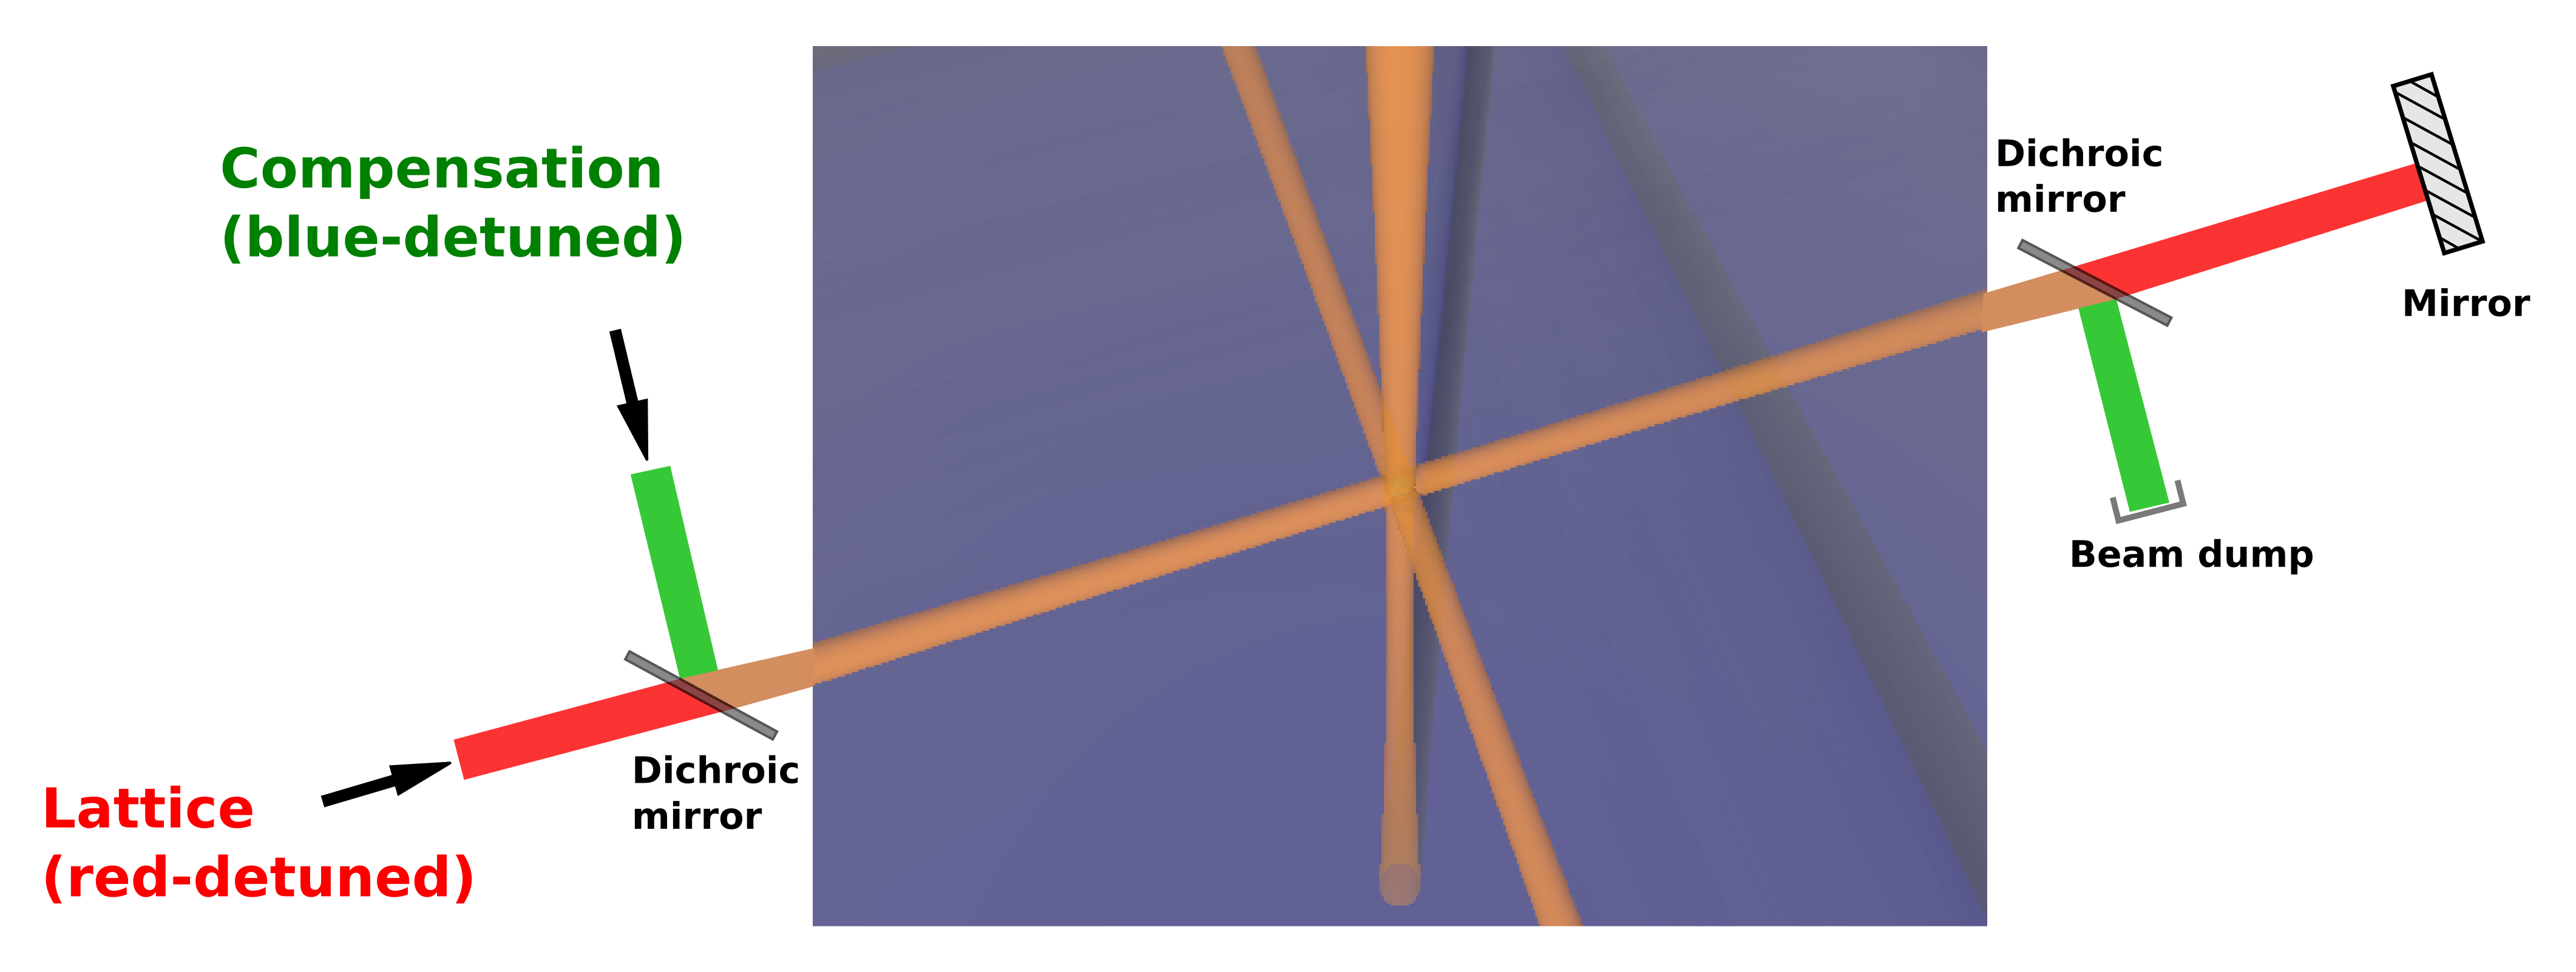
\includegraphics[width=0.8\textwidth]{figures/compensated_lattice_simple_schematic.png}
\caption{Simplified schematic of the compensated lattice
setup}\label{fig:compensated_lattice_simple_schematic}
\end{figure}

The lattice beam that propagates along the $x$ axis produces a potential of the
form 
\begin{equation}
  V_{L}( x; y,z)  = 
  - s_{0} \exp\left[- 2 \frac{ y^{2} + z^{2} }{w_{L}^{2}} \right]
  \cos^{2}( k_{L} x ) 
\end{equation}
where $s_{0}$ is the lattice depth at the center of the potential,  $w_{L}$ is
the lattice beam waist and $k_{L} = 2\pi/\lambda_{L}$ is the wavenumber of the
lattice light.
The compensation beam that propagates along $x$ produces a potential  
\begin{equation}
  V_{C}( x; y, z)  = 
   g_{0}  \exp\left[ -2 \frac{ y^{2} + z^{2} }{w_{C}^{2}} \right] 
\label{eq:Vcomp}
\end{equation}
where  $g_{0}$ is the depth (or rather height since it is repulsive) of the
compensating potential, and $w_{C}$ is the beam waist of the compensation beam.

The combined potential of lattice plus compensation for the beams propagating
along $x$ is 
\begin{equation}
  V_{1D}( x; y ,z ) = V_{L}(x; y,z) + V_{C}(x; y, z)
\end{equation}

The total potential for our simple cubic lattice is given by 
\begin{equation}
  V_{3D}(x, y, z)  =  V_{1D}( x; y,z) + V_{1D}( y; z,x) + V_{1D}(z; x,y)
\end{equation}


In what follows we will study the properties of a two-state spin mixture of
fermionic atoms in the compensated optical lattice potential.  We will first
look at general aspects of the potential, using analytic approximations to its
shape and considering a zero temperature sample.  Then we will use the
high-temperature series expansion (HTSE)\footnote{ The HTSE is  an analytical
solution to the Hubbard model that is valid at high-temperatures.  The HTSE is
very good for $T \gg t$ and works down to $T/t \sim 1.8$.  This solution gives
us the thermodynamic quantities (density, double occupancy, entropy per
particle, etc.)  for a homogeneous system.}  and the local density
approximation (LDA) to explore the properties of the system in more detail. 

\section{General aspects of the potential }

Before we go ahead and deploy the full machinery of the LDA we will discuss
some general aspects of the potential. 

One of the important things to note is that at each point in space  we will, in
general, have three different lattice depths, associated with each of the
$x,y,$ and $z$ lattice directions.  For this reason the potential is difficult
to visualize.  To make things simpler, we can consider the potential along the
111 direction,    along this direction we have equal
lattice depths in $x,y,$ and $z$:
\begin{equation} 
  s_{x}( \rdiag ) = s_{y}( \rdiag ) = s_{z}( \rdiag ) = 
  s_{0} \exp \left[ - \frac{ 4 \rdiag^{2} }{3 w_{L}^{2} } \right]  
  \equiv s(\rdiag) 
\end{equation}
where $\rdiag$ represents the distance along the 111 diagonal line.

The bottom envelope of the lattice potential along 111 is given by 
\begin{equation}
  V_{L,\text{env}}( \rdiag )  = -3 s_{0} 
  \exp \left[ - \frac{ 4 \rdiag^{2} }{3 w_{L}^{2} } \right]  
\end{equation} 


An important aspect of a lattice potential is that the energy spectrum exhibits
a band structure.  The lowest energy of the band, $E_{0}$, measured from the
potential envelope $V_{L,\text{env}}$, can be approximated by the zero-point
energy of the 3D harmonic oscillator obtained by Taylor expanding the potential
at a lattice site.   This approximation is only valid for deep lattices
($\gtrsim 10\,E_{R}$) but we will use it here for its simplicity: 
\begin{equation}
  E_{0} = 
     \frac{3}{2} \hbar \omega_{0}  = 3E_{R}\sqrt{ s/E_{R} } 
\end{equation} 
We can also obtain an expression for the bandwidth $W$, valid in the limit of
deep lattices~\cite{Bloch2008}:
\begin{equation}
  W =   12 t 
  = E_{R}\frac{48}{\sqrt{\pi}} (s/E_{R})^{3/4} e^{-2\sqrt{s/E_{R}}} 
\end{equation}
Notice that the quantities $E_{0}$, $W$, $\omega_{0}$, $s$, and $t$ are all
functions of $\rdiag$. 

The energy of the first excited band in the lattice corresponds to an
excitation along one of the lattice directions, which is an extra $\hbar
\omega_{0}$  above the lowest band.  In Fig.~\ref{fig:lattice_general} we have
plotted the lattice potential envelopes along with the energy boundaries of the
lowest band and a line that is representative of the energy in the  first
excited band.  
\begin{figure}
    \centering
    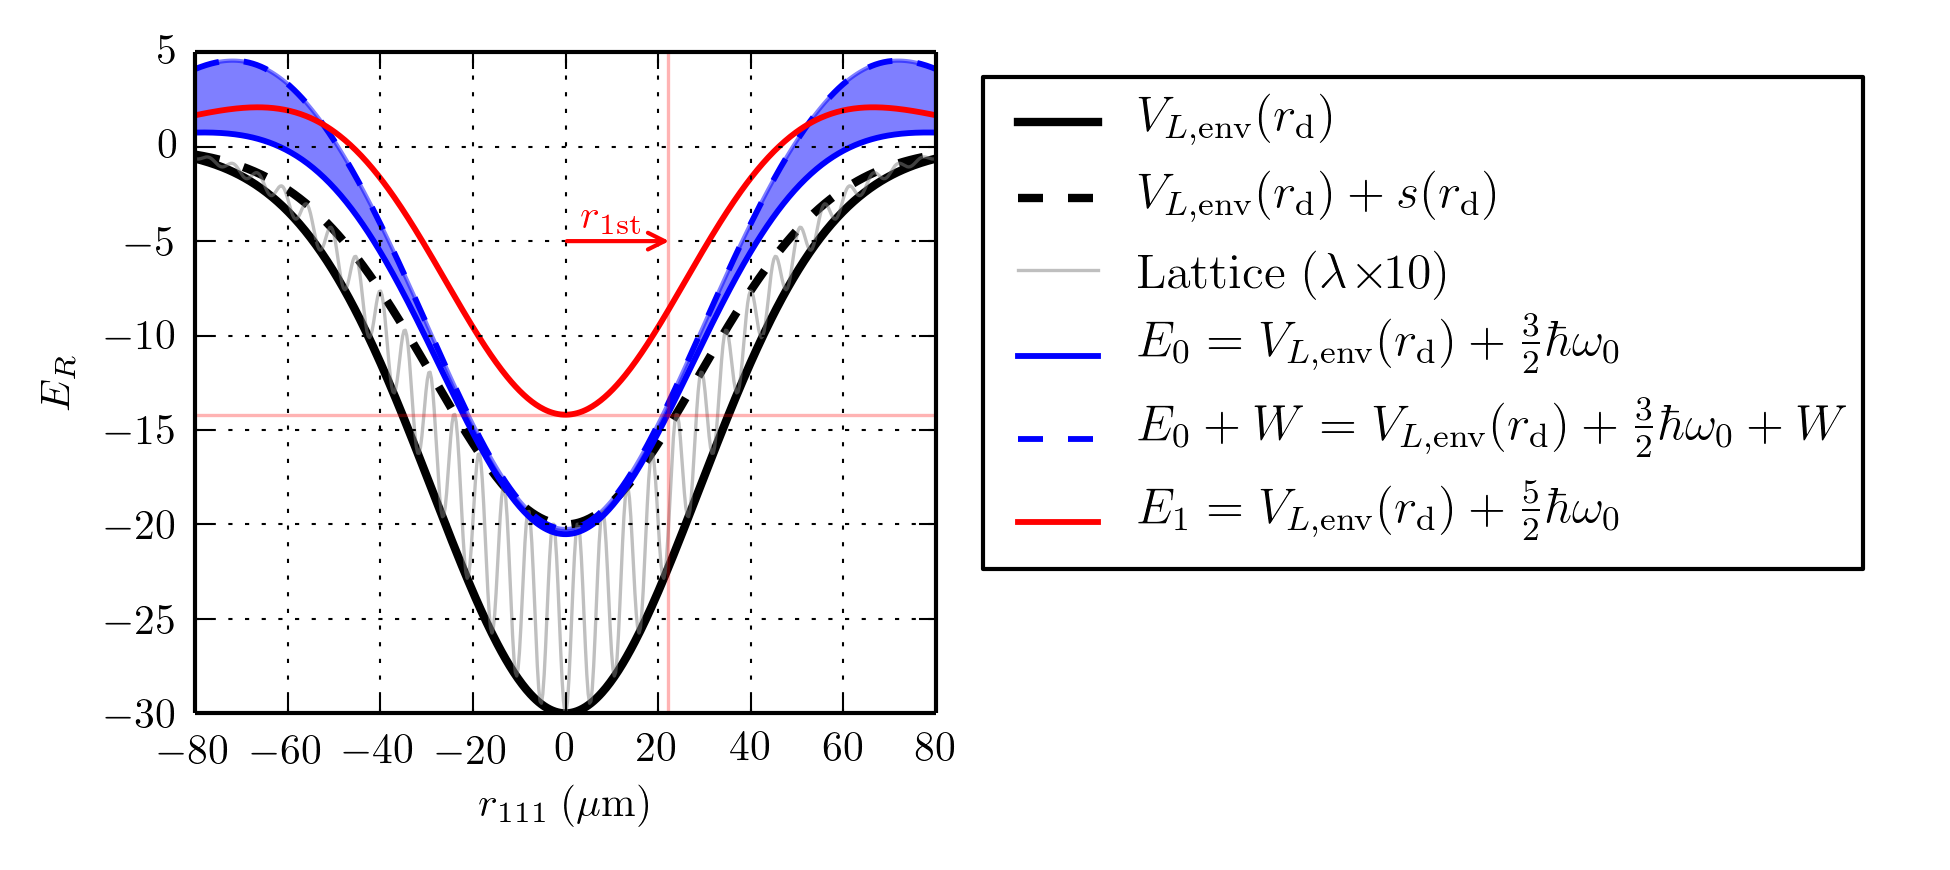
\includegraphics[width=0.8\textwidth]{figures/lattice_general.png}
    \caption{Profiles along $\rdiag$ for a 10$E_{R}$ lattice with $w_{L}=47\,\mu$m. }
\label{fig:lattice_general}
\end{figure}
Also indicated in Fig.~\ref{fig:lattice_general} is the radius,
$r_{1\text{st}}$, at which the energy of the lowest band is equal to the band
gap at the origin:
\begin{equation}
  E_{0}(r_{1\text{st}} )  = 
  E_{1}(0 )  
\end{equation} 
 In order to stay within the single band approximation of the Hubbard model,
our sample needs to have a size that is smaller than $r_{1\text{st}}$.   An
analytical expression for $r_{1\text{st}}$ can be obtained from the quadratic
expansion of $E_{0}$: 
\begin{equation}
 r_{1\text{st}} = w_{L} \left[ \frac{E_{R}\sqrt{s_{0}/E_{R}}}
                              {2s_{0}-E_{R}\sqrt{s_{0}/E_{R}}}  \right]^{1/2} 
\label{eq:r1st} 
\end{equation} 

\subsection{Lattice locking}
\label{subsec:locking}

On occasion we will want to raise the lattice depth suddenly. This will be
useful to get the maximum possible Debye-Waller factor when performing Bragg
scattering,  or to keep the density distribution frozen when sweeping across
the narrow Feshbach resonance to make doublons.   

For Feshbach sweeps across the narrow resonance we have found that going across
from 80\,$a_{0}$ to 61\,$a_{0}$ in 24 ms gives us nearly 100\%
doublon-to-molecule conversion efficiency.  This time perhaps can be reduced by
a factor of two if we approach the resonance quickly and then only slow down
the field ramp as we go across it.   The time it takes to sweep across the
resonance should be much faster than the tunneling time in the locked lattice.
We can aim for a factor of five larger tunneling time than sweep time, which
for sweep times on the order of 10~ms gives $t<20$~Hz which can be achieved
with a lattice depth $\approx 30\,E_{R}$, see Fig.~\ref{fig:lattice_lockA}.  

We can use the expression for $r_{1\text{st}}$ obtained in Eq.~\ref{eq:r1st} as
an estimate of the number of atoms (at a density $n=1$) that we can hold in a
locked lattice without involving higher bands.  We obtain
\begin{equation} 
 N_{1\text{st}} =  \frac{4}{3}\pi \left[ \frac{E_{R}\sqrt{s_{0}/E_{R}}}
                              {2s_{0}-E_{R}\sqrt{s_{0}/E_{R}}}  \right]^{3/2} 
                     \left( \frac{w_{L}}{a} \right)^{3} 
\end{equation}

For a lattice depth $s_{0}=30\,E_{R}$  this corresponds to $r_{1\text{st}} =
0.32 w_{L}$ and $N_{1\text{st}} = 0.13 (w_{L}/a)^{3}$.
Figure~\ref{fig:lattice_lockB} shows a plot of $N_{1\text{st}}$ as a function
of lattice depth for various lattice beam waists.  
%For some measurements we blow away
%any remaining atoms with a resonant light pulse and sweep back across the
%resonance to dissociate the molecules.  For such a procedure we require the
%density distribution to remain locked for times up to 48~ms.  The tunneling
%rate needs to be less than 2~Hz to have less than 0.1 tunneling times in 48 ms.  

%On Fig.~\ref{fig:lattice_lockA} we show the tunneling rate as a function of
%lattice depth, and we see that to achieve 2~Hz one needs $s_{0}\approx
%44\,E_{R}$.  With that in mind we have to consider that as we lock-up the
%lattice to $44\,E_{R}$ we want to stay within the single band Hubbard model.
%Figure~\ref{fig:lattice_lockB} shows the atom number, $N_{1\text{st}}$,
%corresponding to a sample with density $n=1$ atom per site filled up to
%$r_{1\text{st}}$. For atom numbers greater than $N_{1\text{st}}$ the
%single band approximation breaks down.   
\begin{figure}
        \centering
        \begin{subfigure}[t]{0.48\textwidth}
		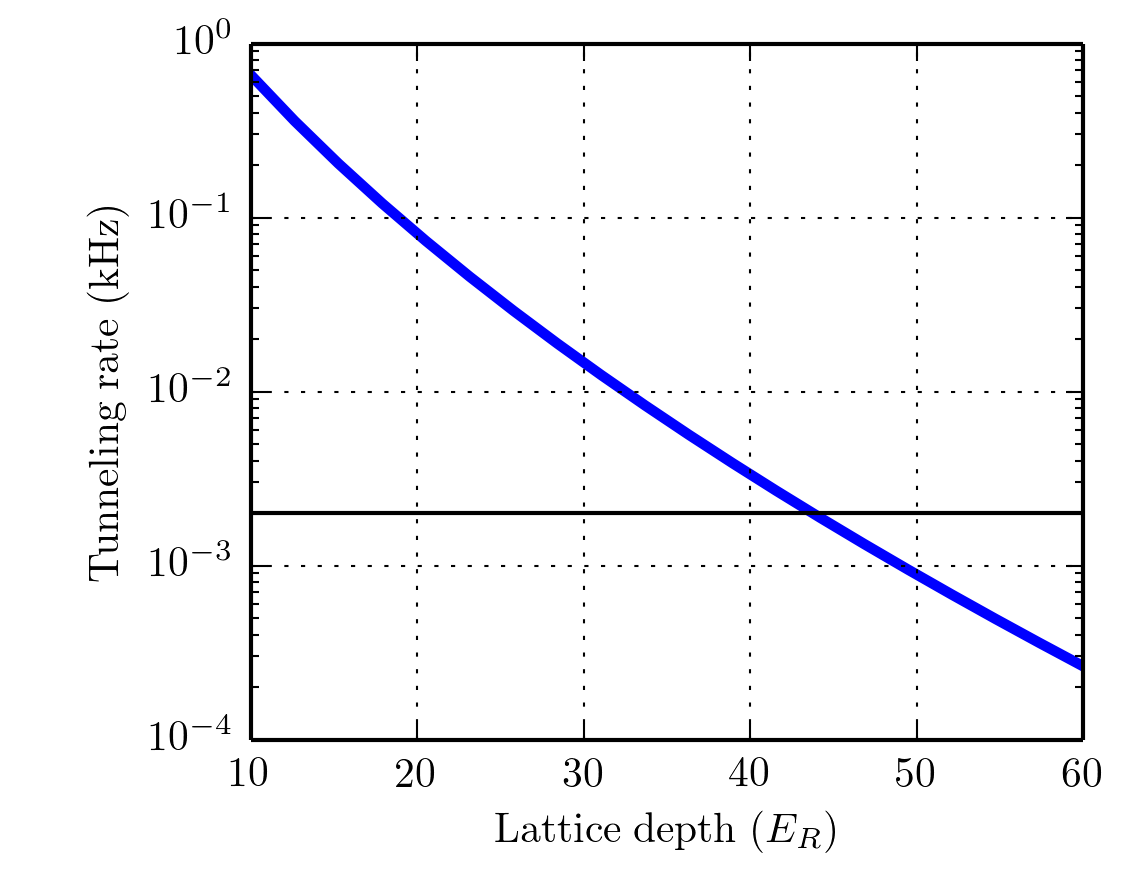
\includegraphics[width=\textwidth]{figures/lattice_tunneling.png}
\caption{Tunneling rate.  The black line is at 2~Hz, which is the rate required
to keep the lattice frozen during a measurement of the double occupancy.}
                \label{fig:lattice_lockA}
        \end{subfigure}
        ~ %add desired spacing between images, e. g. ~, \quad, \qquad etc.
          %(or a blank line to force the subfigure onto a new line)
        \begin{subfigure}[t]{0.48\textwidth}
		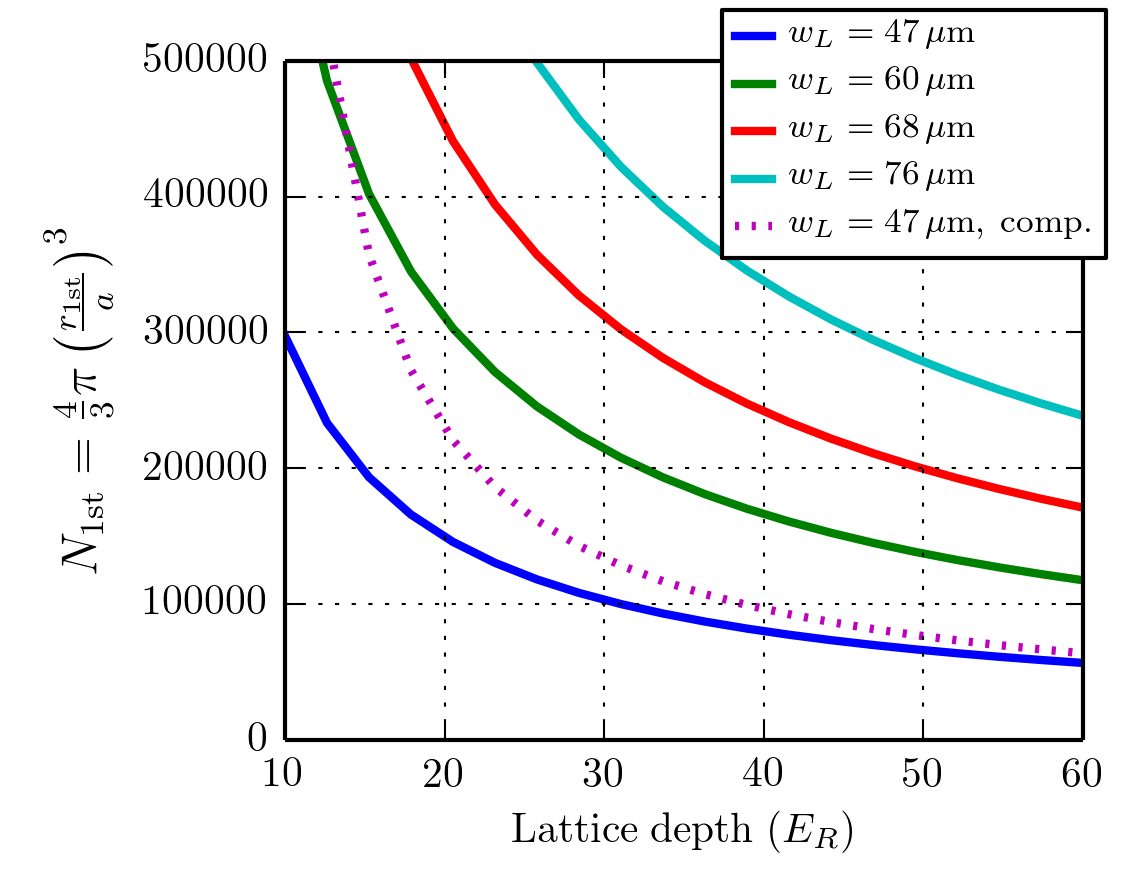
\includegraphics[width=\textwidth]{figures/lattice_lock.png}
\caption{Maximum atom number to stay in the single band regime.  The dashed
line includes 3\,$E_{R}$ of compensation, with a compensation beam waist of
$w_{C}=40\,\mu$m.}
                \label{fig:lattice_lockB}
	\end{subfigure}%
	\caption{Atom number constraints when locking the
lattice.}\label{fig:lattice_lock}
\end{figure}

From Fig.~\ref{fig:lattice_lockB} we see that for samples of $N\!=\!300,000$
atoms and a lattice beam waist of $47\,\mu$m,  the maximum lock depth to stay
in the single band regime is $\approx 10\,E_{R}$.   Currently, when doing Bragg
scattering measurements, we lock the lattice up to 20\,$E_{R}$ to get the
largest possible Debye-Waller factor.   In the Bragg experiment we use a
compensation of 3\,$E_{R}$ to flatten a 7\,$E_{R}$ lattice and we leave the
compensation on as we lock the lattice and probe the sample.  Flattening the
potential with  $3\,E_{R}$ of compensation results in a maximum atom number of
$\approx$230,000 atoms to stay in the single band regime, as is shown with the
dotted line in Fig.~\ref{fig:lattice_lock}.  Our latest experiments with Bragg
scattering use an atom number $N\approx200,000$.  We have observed that locking
the lattice to deeper values, such as 50\,$E_{R}$ and 80\,$E_{R}$ deteriorates
our Bragg signals.


For the measurement of the double occupancy, we have found that Feshbach
molecules scatter green light strongly.  If we shine any green light on them,
we loose them in just a few milliseconds.  This means that, when considering
doublon measurements, we cannot afford to have any green compensation light on.  
With this in mind we see from Fig.~\ref{fig:lattice_lock} that, in order to
lock the lattice up to $30\,E_{R}$  and have the capacity to hold $N\approx
250,000$ in the single band regime, we would require a lattice beam waist as
large as $\approx 65\,\mu$m. 

Our current lattice waist of 47~$\mu$m is an important limitation for our
ability to enhance the Debye-Waller factor when doing Bragg scattering or to
freeze tunneling to measure the double occupancy. 


%%\subsection{Characteristic energy}
%%
%%In the previous subsection we considered the number of atoms required to fill
%%up a sample (at zero temperature and  a density of one per site) up to a
%%certain radius.    For a given number of atoms and a band shape,  that band
%%energy at that radius is (up to some constants that will be specified below)
%%referred to as the characteristic energy of the trap, $E_{\text{t}}$. 
%%
%%
%%For a sample of atoms with radius small compared to the lattice beam waists
%%we can do a series expansion of the  potential envelope and the band bottom to
%%obtain
%%\begin{equation}
%%\begin{split}
%%    \frac{ V_{L,\text{env}}( \rdiag ) }{ E_{R} }  & =   
%%        -3 s_{0}  + \frac{ 4 s_{0} }{w_{L}^{2}} \rdiag^{2}  \\
%%    \frac{ \frac{3}{2}\hbar \omega_{0} }{ E_{R} } & = 
%%        3 \sqrt{ s_{0}} - \frac{ 2 \sqrt{s_{0}}}{w_{L}^{2}} \rdiag^{2} 
%%\end{split}
%%\label{eq:lattice-expand-harmonic}
%%\end{equation}
%%
%%The harmonic approximation to the lowest band in the lattice is then 
%%\begin{equation} 
%%   \frac{ E_{0}(\rdiag) }{E_{R} }  = 
%%       \left(\frac{ 4 s_{0} - 2 \sqrt{ s_{0} } }{ w_{L}^{2} } \right)\rdiag^{2} 
%%       \equiv  \alpha_{\text{t}}  \left( \frac{ \rdiag}{a} \right)^{2}
%%\end{equation}
%%where $a=\lambda/2$ is the lattice spacing.  This defines $\alpha_{\text{t}}$
%%as 
%%\begin{equation}
%% \alpha_{\text{t}} =  \frac{ 4s_{0} - 2\sqrt{s_{0}}}{ (w_{L}/a)^{2} } 
%%\end{equation}
%%The characteristic energy of the trap is defined as
%%\begin{equation} 
%%  \frac{ E_{\text{t}} }{E_{R}} =  \alpha_{\text{t}} \left(  \frac{ 3N }{ 4\pi }
%%\right)^{2/3}
%%\label{eq:characteristic-energy} 
%%\end{equation}
%%where $N$ is the total atom number.  It is seen here that the characteristic
%%energy is the energy of the lowest band at a radius given by 
%%\begin{equation}
%%  \frac{ \rdiag }{ a } =  \left( \frac{ 3N }{ 4 \pi} \right)^{1/3}
%%  \ \ \Rightarrow   \ \ 
%%  N = \frac{1}{d^{3}} \left(   \frac{4}{3} \pi \rdiag^{3}  \right)
%%\end{equation}
%%This radius is simply the size occupied by the $N$ atoms at a density of one
%%atom per site.  
%%
%% 
%%\textbf{Note:} Usually the characteristic energy is defined using the radius of
%%the sample at a density of two atoms per site~\cite{Schneider2010}.  Perhaps
%%this is good if one wants to assess the formation of a band insulator with
%%respect to the band gap.   When dealing with Mott insulating states and
%%comparing $E_{t}$ with the Mott gap, $U$, a density of one atom per site on the
%%definition is the best choice, and the one we adopt here.  
%%
%%
%%The characteristic energy is a useful quantity because it provides a
%%length-scale-free way of assessing  the level of confinement in the
%%trap\footnote{ As an alternative measure of the same concept, the
%%characteristic filling is defined as~\cite{Jordens2010}.
%%\begin{equation} 
%%    \rho_{\text{t}} = N \left( \frac{ \alpha_{t} }{ 6 t } \right)^{3/2}
%%    =  \frac{8\pi}{3} \left( \frac{ E_{\text{t}} }{ 6 t}   \right)^{3/2}  
%%\end{equation}
%%Using the characteristic filling it is a little bit more cumbersome to quickly
%%get an idea of the length-scale-free filling as one has to convert the
%%interaction energy to an effective density in order to make a well informed
%%comparison.   It is always easier to just compare $U$ to $E_{t}$. }.
%%Regardless of the waist of the lattice beams, for a given interaction strength
%%$U$, a Mott-insulating core  at the center of the sample  can be achieved if
%%$E_{\text{t}} \approx U/2 $.   Notice that such a characteristic energy
%%can be achieved experimentally in either of two ways: changing the confinement,
%%$\alpha_{\text{t}}$, or changing the atom number, $N$.  
%%
%%
%%To give an example of the use of the characteristic energy, we consider our
%%current setup with a beam waist $w_{L}=47\,\mu$m.   In a 7\,$E_{R}$ lattice
%%(without compensation)
%%\begin{equation}
%%\begin{split}
%%  \alpha_{\text{t}} & =  2.909 \times 10^{-3} \\
%%   t & = 4.88 \times 10^{-2}\,E_{R}  \\ 
%%\end{split}
%%\end{equation}
%%With an interaction strength $U/t = 24$, the atom number required to make an
%%insulating state with $n=1$ at the center is 
%%\begin{equation} 	
%% N = \frac{4\pi}{3}  
%%    \left(  \frac{ U/E_{R} }{ 2 \alpha_{\text{t}} } \right)^{3/2}  
%%     \approx 12,000 \ \text{atoms}  
%%\end{equation}
%%We will see in a later section that this estimate agrees with the full
%%machinery of the LDA.  
%%
%%In actual experiments typically the main constraint is the atom number.  The
%%shape and depth of the traps can be adjusted around the achievable atom number
%%such that one can access the phases of interest.  In our case these are
%%the Mott insulator state and the antiferromagnetic Mott-insulator
%%which both require a density of one atom per site at the center.  
%%
%%
%%A plot of $E_{\text{t}}/t$ as a function of lattice beam waist for a fixed atom
%%number, $N$=500,000 is shown in Fig.~\ref{fig:Et-waist}.   We use a black line
%%to denote the value of $U/2t$ for a scattering legth of 650$a_{0}$ in a
%%10\,$E_{R}$ lattice.  We see that achieving half-filling with the confinement
%%provided only by the red-detuned lattice requires a lattice beam waist of
%%$\approx 160\,\mu$m.  
%%\begin{figure}
%%    \centering 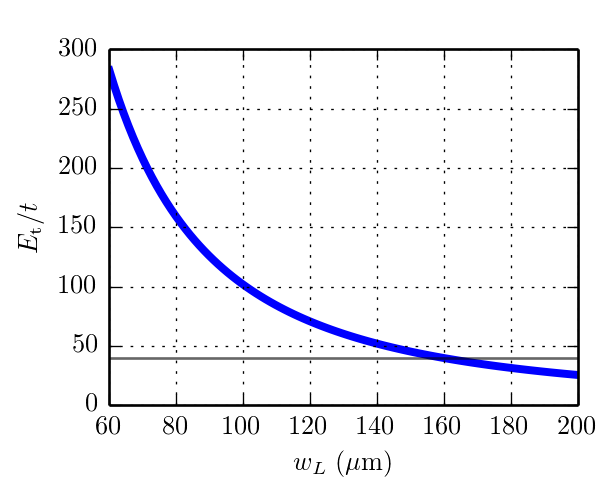
\includegraphics[width=0.5\textwidth]{figures/Et-waist.png}
%%\caption{Characteristic energy as a function of beam waist for $N=500,000$
%%atoms. The black line denotes $U/2t$,  which should be the
%%characteristic energy required to obtain a half-filled sample at the center of
%%the potential.}
%%\label{fig:Et-waist}
%%\end{figure}
%%In the next section we will see how the addition of the compensating potential
%%can help us achieve a Mott insulating state using a smaller waist lattice for
%%the lattice beams.


\subsection{Compensation}
\label{subsec:compensation}


We are interested in exploring the idea of evaporative cooling in a lattice and
also the concept of the entropy capacity of the lattice system.  We will see
that for both these two ideas it will be necessary to introduce the concept of
compensation.  

Compensation is a way of flattening the profile of the lowest band in order to
enlarge the central region of the sample which may exhibit the phase of
interest.   Using a smalll lattice beam waist and compenation beams has two
important effects~\cite{Mathy2012}:
\begin{itemize}
\item  The extent of the the phase of interest (Mott state or AFM) in the
trapped sample can be enlarged by flattening the potential.   An limiting case
of this would be a square well potential.  With compensation beams the
potential can be made quartic instead of quadratic.  
\item  With a small lattice beam waist, the use of compensation enables the
possibility of evaporative cooling the sample in the lattice.  
\end{itemize} 

With the addition of repulsive compensation beams with depth $g_{0}$ and beam
waist $w_{C}$,  as in Eq.~\ref{eq:Vcomp},  we can expand the lowest band
profile of the lattice in a power series as  
\begin{multline} 
  E_{0}(\rdiag)    \approx   
  3( g_{0} + E_{R}\sqrt{s_{0}/E_{R}} - s_{0} )   
  + \left[ 
    \frac{ 4s_{0} - 2E_{R}\sqrt{s_{0}/E_{R}} }{w_{L}^{2} } 
   - 
  \frac{ 4 g_{0} }{ w_{C}^{2}} \right]
  \rdiag^{2}  \\ 
  +  \left[  \frac{ - 8 s_{0} + 2E_{R}\sqrt{s_{0}/E_{R}} }{3 w_{L}^{4} } + 
    \frac{ 8 g_{0} }{3 w_{C}^{4} }  \right] \rdiag^{4}   + 
  \mathcal{O}( \rdiag^{6} )
\end{multline}  

\paragraph{Enlarging the Mott plateau} 
If our interest is to maximally flatten the band profile, we see that we can
completely cancel the quadratic term in the series expansion by choosing 
\begin{equation}
 g_{0} = \frac{  4 s_{0} - 2 \sqrt{s_{0}} }{ 4 \awaist^{2} }  
  \equiv g_{\text{quartic}} 
\end{equation}
where we define  the beam waist ratio $\awaist = w_{L}/w_{C}$ as
in~\cite{Mathy2012}.  This choice of $g_{0}$ will be the most favorable in
enlarging the size of the $n=1$ region of the cloud.
 
We point out that, for $\awaist > 1$,  if we
use a compensation larger than $g_{\text{quartic}}$, the band profile would
have a bump in the center.  We have observed experimentally that in that case
it becomes hard to align the compensation beams such that the sample actually
stays at the center of the trap.

In our current experiments we use $s_{0}$=7\,$E_{R}$ and our beam waists are
approximately $w_{L}=47\,\mu$m and $w_{C}=40\,\mu$m, which gives
$\awaist=1.17$.  The necessary compensation to flatten the band would be
$g_{\text{quartic}} =  4.1\,E_{R}$




\paragraph{Evaporation.} We want to consider the possibility of evaporative
cooling in a sample that has $n=1$ at the center.  To impose $n=1$ at the
center we set the global chemical potential (measured from the lowest point
along the band profile) at $\mu_{\text{global}} = U/2$, where $U$ is the
on-site interaction strength.   

At zero temperature, $\mu_{\text{global}}$  can be obtained as the
value of the band profile at the radius that defines the edge of the cloud.  In
this way, the half-filling requirement can be written as 
\begin{equation}
    \mu_{\text{global}} =  E_{0}(r_{\text{hf}}) - E_{0}(0) = U/2 
  \label{eq:half-filling-radius} 
\end{equation} 
which defines the radius of the half-filled sample, $r_{\text{hf}}$.  The situation is illustrated in Fig.~\ref{fig:lattice_general-comp}. 
\begin{figure}
    \centering
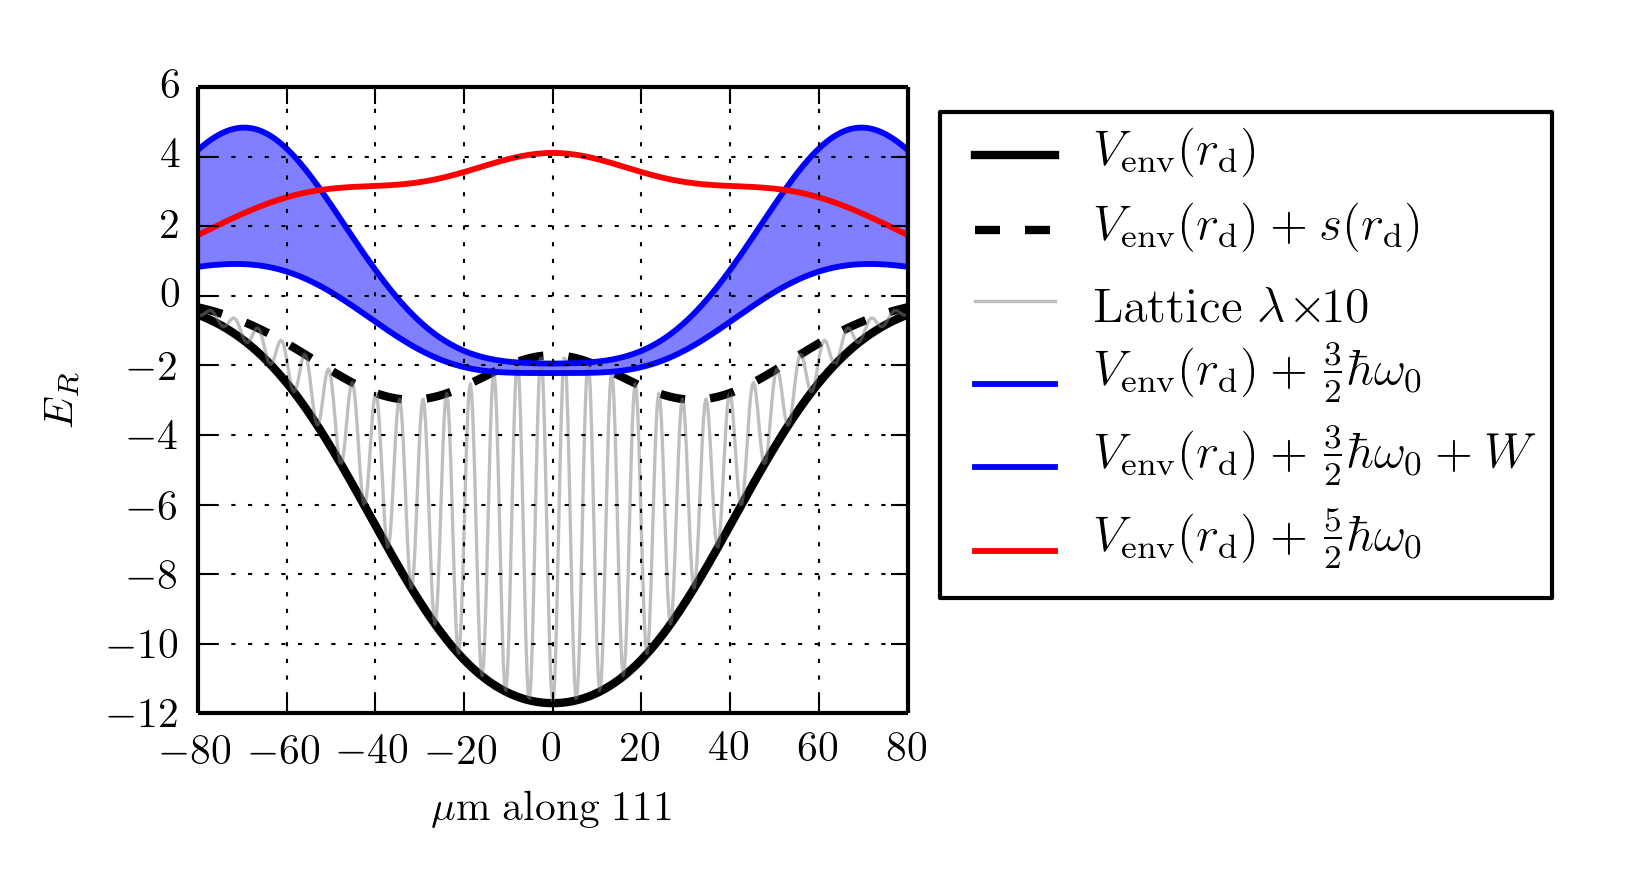
\includegraphics[width=1.0\textwidth]{figures/lattice_general-comp.png}
\caption{Profiles along $\rdiag$ for a 7\,$E_{R}$ lattice with
$w_{L}=47\,\mu$m.  The compensation is $g_{0}=g_{\text{quartic}}$, and the
chemical potential is set at $U/2$ to achieve half-filling.  This conditions
determine the waist ratio $\awaistevap=1.17$ such that the chemical potential
also matches the evaporation threshold.  The figure on the left shows the
profile of the  lattice potential, which illustrates how the energy scales of
the potentials are significantly larger than the energy scales of the
Fermi-Hubbard parameters $U$ and $t$.   The figure on the right is a zoomed in
version of the one on the left.   }
\label{fig:lattice_general-comp}
\end{figure}


In order to maximize the evaporation rate for a half-filled sample we need
$E_{0}(r_{\text{hf}})$ to come as close as possible to the evaporation
threshold energy, $E_{\text{th}}$.  In our setup the threshold is the energy
required to escape along one of the lattice beams: 
\begin{equation} 
  E_{\text{th}} =  g_{0} + E_{R}\sqrt{s_{0}/E_{R}} - s_{0}  \equiv E_{0}(0)/3 
\end{equation}

The evaporation rate is maximized if $E_{0}(r_{\text{hf}}) = E_{\text{th}} $.
This condition along with Eq.~\ref{eq:half-filling-radius}, results in
\begin{equation}
  E_{0}(0)/3  = U/2 + E_{0}(0) \ \ \ \ \ \Rightarrow \ \ \ \ \ 
  -2( g_{0} + E_{R}\sqrt{s_{0}/E_{R}} - s_{0} ) = U/2  
  \label{eq:optimal-evap} 
\end{equation} 
 
To maximize the size of the Mott plateau we set $g_{0} = g_{\text{quartic}} =
\frac{  4 s_{0} - 2 \sqrt{s_{0}} }{ 4 \awaist^{2} } $, and then we solve for
the beam waist ratio $\awaistevap$, which produces the best conditions for
evaporation in the lattice: 
\begin{equation}
 \awaistevap^{2} =  \frac{ 4 s_{0} - 2 E_{R} \sqrt{s_{0}/E_{R} }}
    { 4s_{0} - 4 E_{R} \sqrt{s_{0}/E_{R}}  - U }  
\end{equation} 
\begin{figure}
    \centering
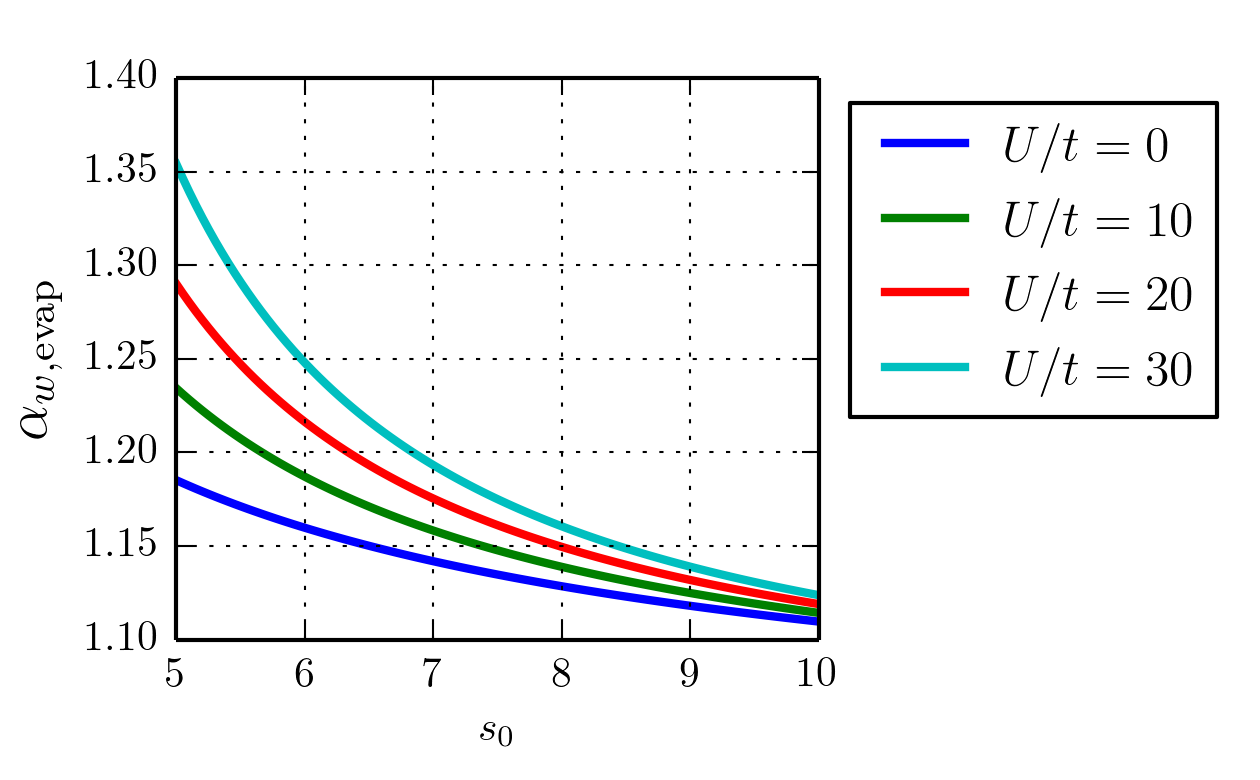
\includegraphics[width=0.7\textwidth]{figures/alpha-evap-optimal.png}
\caption{Optimal beam waist ratio for enlarging the central flat portion on
the band and maximizing the rate of evaporative cooling. }
\label{fig:alpha-evap-optimal}
\end{figure}
In Fig.~\ref{fig:alpha-evap-optimal} we show plots of $\awaistevap$ for various
values of $U/t$.  We can see that for a 7\,$E_{R}$ lattice $\awaistevap$ is
between 1.15 and 1.20.  

We can conclude from the analytical considerations presented in this section
that a compensated lattice with a value of $\awaist \approx 1.17 $ will offer
the best scenario for evaporation while flattening the bottom of the band.  


%For a deep lattice ($\gtrsim 10\,E_{R}$) the on-site interactions can be
%expressed analytically as \begin{equation} \frac{U}{E_{R}}  =  4 \sqrt{2\pi}
%\frac{ a_{s} }{\lambda}  (s/E_{R})^{3/4} \label{eq:onsite-analytic}
%\end{equation} The scattering length is usually expressed in units of the Bohr
%radius, $a_{0}$, so it is useful to keep in mind that for our 1064~nm lattice
%$\lambda = 20113\ a_{0}$.  In our experiment we want to avoid very large
%scattering lengths because they give rise to fast inelastic losses that scale
%as $a_{s}^{4}$; reasonable values of $a_{s}$ are up to 800\,$a_{0}$.   In a
%7\,$E_{R}$ lattice a scattering length $a_{s}=800\,a_{0}$ implies an
%interaction strength $U/t=35$, calculated from Eq.~\ref{eq:onsite-analytic}.


\subsection{Practical considerations} 

\paragraph{Atom number} We now turn to examine the number of atoms required in
order to achieve half-filling in the optimal setup.   To get this number we
need to find the half-filling radius, $r_{\text{hf}}$,  which is defined by
Eqs.~\ref{eq:half-filling-radius} and~\ref{eq:optimal-evap}.  Using a density
of one atom per site we can find the atom number from the radius, as
$N_{\text{hf}} = \frac{4}{3} \pi (r_{\text{hf}}/a)^{3}$,  where $a$ is the
lattice spacing ($a=\lambda/2$). 

To solve Eqs.~\ref{eq:half-filling-radius} and~\ref{eq:optimal-evap} we can use
the power series expansion of the band energy, which for
$g_{0}=g_{\text{quartic}}$ is 
\begin{equation}
  E_{0}(\rdiag) - E_{0}(0) = \left[  
  \frac{  2E_{R}\sqrt{s_{0}/E_{R}} - 8s_{0} 
   + 4( 2s_{0} -E_{R}\sqrt{s_{0}/E_{R}} ) \awaist^{4} }
  { 3 w_{L}^{4} } \right] \rdiag^{4} 
\end{equation}
The solution for $r_{\text{hf}}$ is then 
\begin{equation}
  r_{\text{hf}} =  \frac{w_{L}}{\awaist} \left[ 
  \frac{3}{2}  
  \frac{( 1 - 2\awaist^{4} + 2 \sqrt{s_{0}/E_{R}}( \awaist^{4} -1 ) )}
  { ( 1 -  2\awaist^{4} + 4 \sqrt{s0/E_{R}} ( \awaist^{4} -1 ) ) } 
  \right]^{1/4} 
\end{equation}
For $s_{0}=7$ and $\awaist=1.17$ this gives  $r_{\text{hf}}\approx 0.7 w_{L}$.
For a lattice beam waist $w_{L}=47\,\mu$m  this amounts to
$N_{\text{hf}}=990,000$ atoms.    The fully optimized situation for
$w_{L}=47\,\mu$m is shown in Fig.~\ref{fig:lattice_general-comp}. 
 

%When using compensation we will find that we can use smaller beam waists and
%that the potential has the capacity to accommodate a larger number of atoms.
%Since the size of the sample starts becoming comparable to the lattice beam
%waist, we can no longer work in the harmonic approximation.   In later
%sections we will turn to the more precise implementation of the local
%density approximation, and we will calculate the relevant local quantities
%($U$, $t$, etc. ) numerically, without making any deep lattice or harmonic
%approximations. 
% 

\paragraph{Considerations for our current setup}

In our current setup we use a lattice depth $s_{0}=7\,E_{R}$, and we have
approximately $w_{L}=47\,\mu$m and $w_{C}=40\,\mu$m,  which amounts to
$\awaist=1.175$.   As we have seen above, we should compensate this sample with
$g_{\text{quartic}} = 4.11\,E_{R}$ and populate it with $N\approx 990,000$
atoms.  This would yield a half-filled sample with optimal conditions for
evaporative cooling in the lattice.   

Unfortunately we only have $\approx$300,000 atoms at our disposal.   This
forces us to reduce the compensation below $g_{\text{quartic}}$  in order to
achieve $n=1$ at the center.   Reducing  the compensation significantly affects
the prospects of evaporative cooling in the lattice.   
 
At the moment we use the following compensations for each of the three axes:
\begin{center}
\begin{tabular}{ c|c|c|c}
   axis & 1 & 2 & 3 \\
   \hline
   $g_{0}$ & 3.65 &  3.90 & 2.9 \\ 
\end{tabular}
\end{center}
With these values we have found empirically that we can obtain the same
confinement frequencies in all three directions (which produces spherically
symmetric samples) and that we can achieve $n=1$ at the center with
$N\approx300,000$ atoms.  


\paragraph{Why is our atom number 300,000?}   At the moment our
experimental sequence consists of the following steps:
\begin{enumerate}
\item  Evaporate into a dimple potential with a depth of $\approx 0.5\,E_{R}$
per axis.   The cold sample in the dimple has a density of nearly one atom
per site.  

\item  Rotate the polarization of the retro beams to go from dimple to lattice
configuration.   We want the sample in the dimple to have a Fermi energy $E_{F}
< E_{R}$ so that we can be sure that all of the atoms will remain in the lowest
band  as we rotate to a lattice potential.   While we rotate we add a minimal
amount of compensation, 0.06\,$E_{R}$.  

\item  Ramp up the lattice depth in 25 ms up to the point where the lowest band
and first excited band separate, which corresponds to a lattice depth of
$\approx 2.4\,E_{R}$.  At the same time add 0.65\,$E_{R}$ of compensation.
During this time also ramp the interaction strength from the evaporation value
to the value we want in the experiment.  

\item Ramp up, in 15 ms,  the lattice depth to 7\,$E_{R}$ and the compensation
to the desired final value.
\end{enumerate}

So far in our experiments we have tried to keep the density at one per site
from the moment we start in the dimple at Step 1, up to the final sample in
the lattice.    Keeping the density at $n=1$ gives us a constraint for the
number of atoms that we start with in the dimple potential.   We derive this
below. 

In the dimple, having a peak density of one per site translates into having a
global trap Fermi energy which is $E_{F,\text{trap}} \approx E_{R}$.   The
local Fermi energy and the density at the center of the trap can be related by
$E_{F} = \frac{\hbar}{2m} ( 3\pi^{2} n)^{2/3}$.  Setting the density to one per
site, $n=a^{-3}$ yields  $E_{F} = (3/\pi)^{2/3} E_{R} \approx 0.97 E_{R}$.
The local Fermi energy at the center will be the same as the global Fermi
energy of the harmonic trap, so we can find the total trapped atom number from 
\begin{equation}
  E_{F,\text{trap}} = \hbar \omega ( 3 N )^{1/3}  = E_{R}  
 \ \ \ \  \Rightarrow  \ \ \ \  N = \frac{1}{3} 
  \left( \frac{ E_{R}} {\hbar \omega} \right)^{3} 
\end{equation} 

A dimple potential with depth $V_{0}$ per axis has a trapping frequency 
\begin{equation}
  \omega  =  \left( \frac{8V_{0} } { mw_{L}^{2} } \right)^{1/2}
  =   \frac{ a \sqrt{2E_{R}} }{ \hbar \pi} 
   \left(  \frac{8V_{0} } { w_{L}^{2} } \right)^{1/2}
  =   \frac{ 4 a  }{ \hbar \pi w_{L} } 
   \left(  E_{R}V_{0}  \right)^{1/2}
\end{equation} 
so 
\begin{equation} 
 N = \frac{1}{3} 
  \left(  \frac{ \pi w_{L} }{ 4a} \right)^{3}  
  \left( \frac{ E_{R} }{V_{0}} \right)^{3/2} 
\end{equation}
With $V_{0} = 0.5\,E_{R}$ and $w_{L}=47\,\mu$m we obtain $N = 315,000$ atoms. 

Just notice that for this calculation to make sense, the depth of the dimple
potential has to be larger than the Fermi energy in the harmonic trap, that is 
\begin{equation}
  2 V_{0} >  E_{F,\text{trap}}
\end{equation} 
In our setup we just match this condition since $2V_{0}= 1\,E_{R}$ and
$E_{F,\text{trap}} = 1\,E_{R}$.  
 
\paragraph{Can we load more atoms into the lattice?}  In order to load more
atoms into the lattice we would have to start with a larger number of atoms in
the dimple.  If we were to initially load a deeper dimple then, for our beam
waists, the sample would have a density larger than one per site at the center.
This poses a problem because the Fermi energy would be larger than 1\,$E_{R}$,
and it would lead to population of the first excited band when rotating into
the lattice.  Furthermore we do not know if we can achieve as low
temperatures as we do in the 0.5~\,$E_{R}$ dimple.   

A simple way to circumvent the higher band issue would be to compensate the
dimple before rotating the polarization of the retro beams.  In that way, a
larger atom number can be accommodated at a density of one atom per site, and we
could proceed with the ramps that maintain the density at that value.  With a
larger atom number we would find that we would require a larger $g_{0}$, closer
to $g_{\text{quartic}}$, in order to get to half-filling in the final sample.  


\paragraph{Why do we stick with 300,000 atoms?}  We go back to the first
consideration of this section:  locking the lattice.   If we load a sample of
more than $N=230,000$ atoms the lattice lock to 20\,$E_{R}$ compromises our
measurement by forcing atoms into the first excited band.   Already at our atom
number of $N\approx 300,000$ the lock to 20\,$E_{R}$ poses somewhat of a
compromise.

\paragraph{Considerations for future improvements.}  The main bottleneck for
our setup at the moment is related to the lock.  A lattice beam waist of
$w_{L}=70\,\mu$m  would allow us to lock up to 35\,$E_{R}$ with a sample of
$N=300,000$ atoms.   

In the next section we will use the quantitative results of the LDA to gain
more insight into the compensated lattice setup and help us decide on the best
parameters for the future improvements of our setup. 


\section{ Local density approximation }
\label{sec:lda}

In the local density approximation (LDA) we consider each point in our
potential as an homogeneous system and we set the condition that all of these
local homogeneous systems are in thermal equilibrium with each other  at some
temperature $T$.   At each point in our potential we can obtain a local value
of the lattice depth and the on-site interactions. These two quantities
determine the local values of the Hubbard parameters $t$ and $U$.  With these
in hand, we can use a known solution to the homogeneous Hubbard model and
obtain local values for the thermodynamic quantities, such as density, double
occupancy, entropy, etc.   We can then plot the local thermodynamic quantities
as a function of trap position and obtain trap profiles.   

\begin{figure}
    \centering
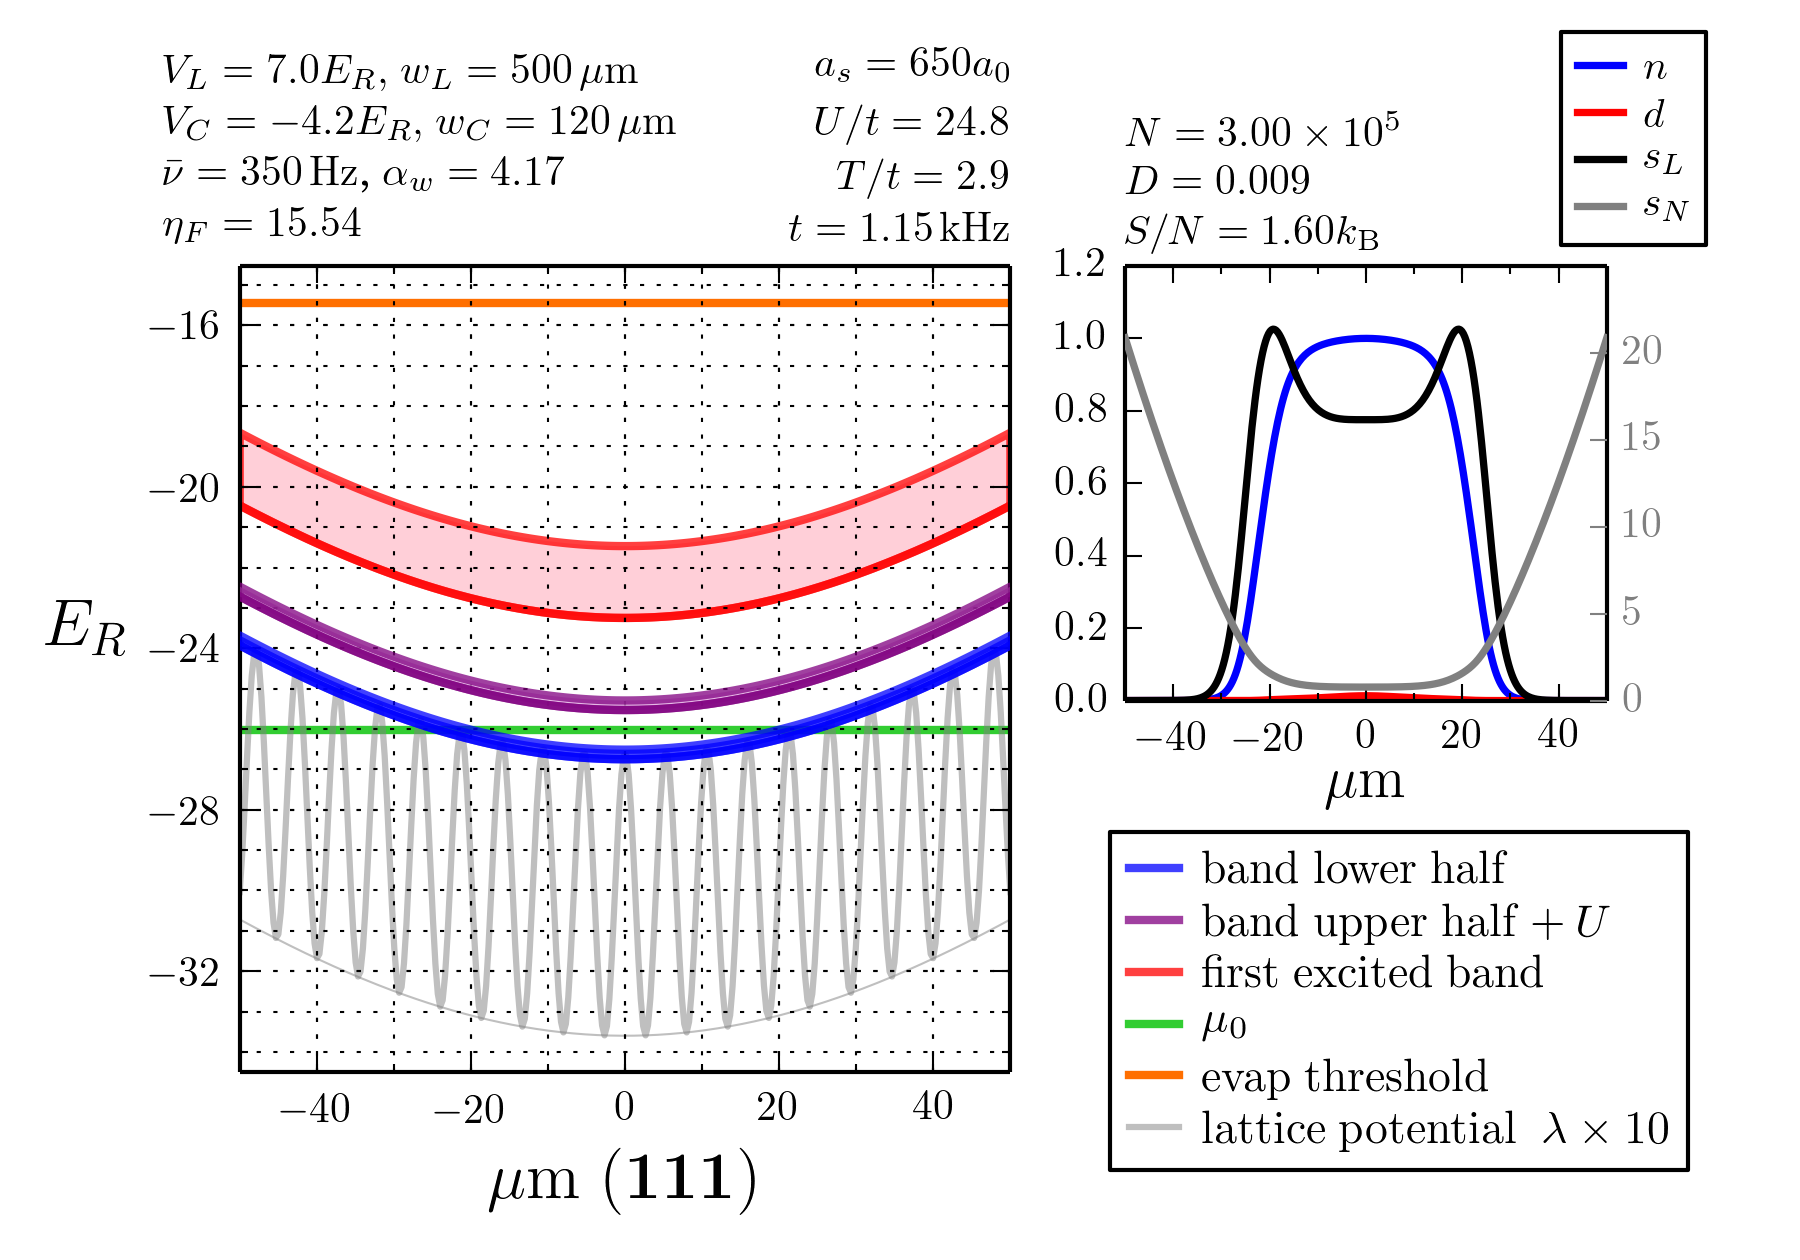
\includegraphics[width=0.75\textwidth]{figures_hubbard-lda/harmonic.png}
\caption{Red detuned uniform lattice with additional harmonic confinement.  The
confiment is adjusted so that the density is one per site at the center with
$N=300,000$ atoms.   The temperature is adjusted such that the overall entropy
per particle is $S/N=1.6k_{\text{B}}$. }  
      \label{fig:HTSE_LDA_harmonic}
\end{figure} 
An example of the LDA for a  uniform lattice potential plus harmonic
confinement is shown in Fig.~\ref{fig:HTSE_LDA_harmonic}.  Notice that to
obtain the uniform lattice plus confinement we use large values of the beam
waists for the lattice and compensation beams, and we use a negative depth for
the compensation beam.  The resulting trap frequencies in this setup are
$\bar{\nu} = 342\,\mathrm{Hz}$ in all three directions, calculated for
$^{6}$Li. 

In plots like the one in Fig.~\ref{fig:HTSE_LDA_harmonic} we show several lines
and regions, and also there are multiple informative labels shown at the top.
Below we give the explanation for each of the lines and labels that are shown.
 
\paragraph{Parameters of the potential.}  The labels on the top left indicate
the depth of the lattice and compensating potentials in recoils, and also the
waists used for the lattice and compensating beams.   The general geometry of
the potential is described in \S\ref{sec:compensated-optical-lattice}.  Also
shown are the beam waist ratio, $\awaist$ and the confinement frequency
$\bar{\nu}$, which is calculated from the curvature of the bottom of the lowest
band. 

\paragraph{Hubbard parameters.}  The labels of on the top right of the main
plot indicate the scattering length and the resulting Hubbard paraemters for
the given the lattice depth.  The values of $U/t$, $T/t$, and $t$ given are
valid at the center of the sample.  Due to the finite lattice beam waist the
tunneling increases as one moves away from the center, and so $U/t$ and $T/t$
decrease monotonically for larger distance from the center.  

\paragraph{Band lower half.}  This region is defined by two lines, the bottom
line corresponds to the lowest energy level accessible to a single particle in
the local  Hubbard hamiltonian.   The top line corresponds to the energy level
exactly in the center of the lowest energy band.      In the absence of
interactions, the Hubbard hamiltonian for a single particle is simply 
\begin{equation} 
  H  = -\frac{\hbar^{2}}{2m} \frac{ \partial }{ \partial x^{2} } +  
       V_{0} \sin^{2}(kx)  
\end{equation}   
The energy level structure as a function of lattice depth is as shown in
Fig~\ref{fig:Hubbard-firstquant}.   In second quantized form the hamiltonian
(without interactions) is usually written as  
\begin{equation} 
  H  = -t \sum_{ \langle ij \rangle, \sigma } a_{i\sigma}^{\dagger} a_{j\sigma} 
  \label{eq:Hubbard-free-secondquant}
\end{equation}  
What is typically not mentioned is that writing the hamiltonian as in
Eq.~\ref{eq:Hubbard-free-secondquant} implies a lattice-depth-dependent  shift
of the energy zero, such that the band structure looks like in
Fig.~\ref{fig:Hubbard-secondquant}.   When solving the Hubbard model using the
HTSE we used the hamiltonian in Eq.~\ref{eq:Hubbard-free-secondquant}, so
energies like the chemical potential are referenced from the center of the
lowest band.    Most importantly, the center of the lowest band is a ubiquitous
energy in the Hubbard model because states below that energy will be almost
unperturbed by interactions, wheras states above that energy will be affected
significantly by interactions. 
\begin{figure}
        \centering
        \begin{subfigure}[t]{0.4\textwidth}
		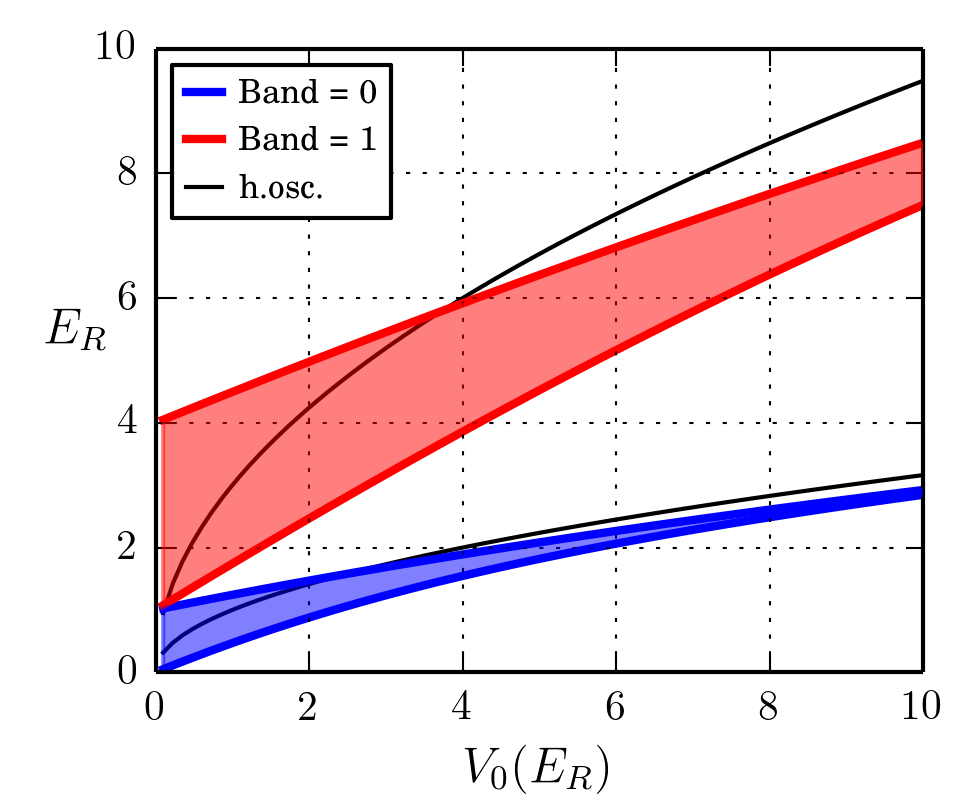
\includegraphics[width=\textwidth]{figures/bands1d_V0_firstquant.png}
\caption{ Band structure when the zero of energy is at the bottom of the
lattice sites.  The zero of energy does not change with lattice depth, and the
band energies go up almost like the harmonic oscillator state in an individual
lattice site.  }
                \label{fig:Hubbard-firstquant}
        \end{subfigure}%
        ~~ %add desired spacing between images, e. g. ~, \quad, \qquad etc.
          %(or a blank line to force the subfigure onto a new line)
        \begin{subfigure}[t]{0.4\textwidth}
		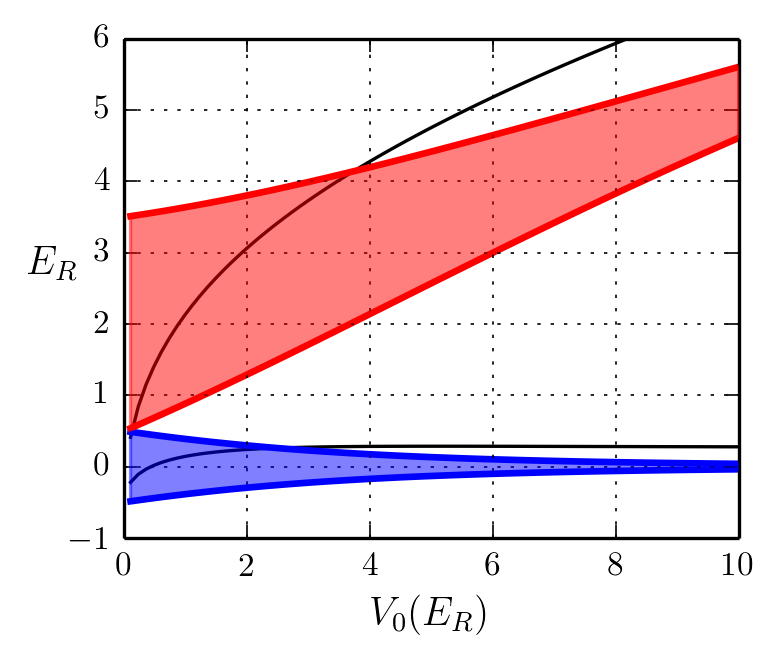
\includegraphics[width=\textwidth]{figures/bands1d_V0_secondquant.png}
\caption{ Band structure when the zero of energy is at the center of the lowest
band.  This shift is implicit when the hamiltonian is written in second
quantized form as in Eq.~\ref{eq:Hubbard-free-secondquant}.  }
                \label{fig:Hubbard-secondquant}
        \end{subfigure}
	\caption{ Band structure in the Hubbard model.  }
\label{fig:Hubbard-first-second}
\end{figure}

\paragraph{Band upper half + $U$. }  As we just pointed out in the last
paragraph, the states above the center of the lowest band will be modified
signficantly by the interactions.  These states will acquire an extra energy
$U$,  this can be seen for instance if we solve the Hubbard model
\begin{equation} 
  H  = -t \sum_{ \langle ij \rangle, \sigma } a_{i\sigma}^{\dagger} a_{j\sigma}
      + U \sum_{i} n_{i\spup} n_{i\spdn}  - \mu\sum_{i,\sigma} n_{ i,\sigma}
  \label{eq:Hubbard-U-secondquant}
\end{equation} 
in a two-lattice system at half-filling.  The solution to this hamiltonian,
using exact diagonalization is shown in Fig.~\ref{fig:exactdiag_2site}.  It can
be seen that the two lower energy levels suffer little change as the
interaction are increased, whereas the two higher energy levels are shifted
upwards by $U$. 
\begin{figure}
    \centering
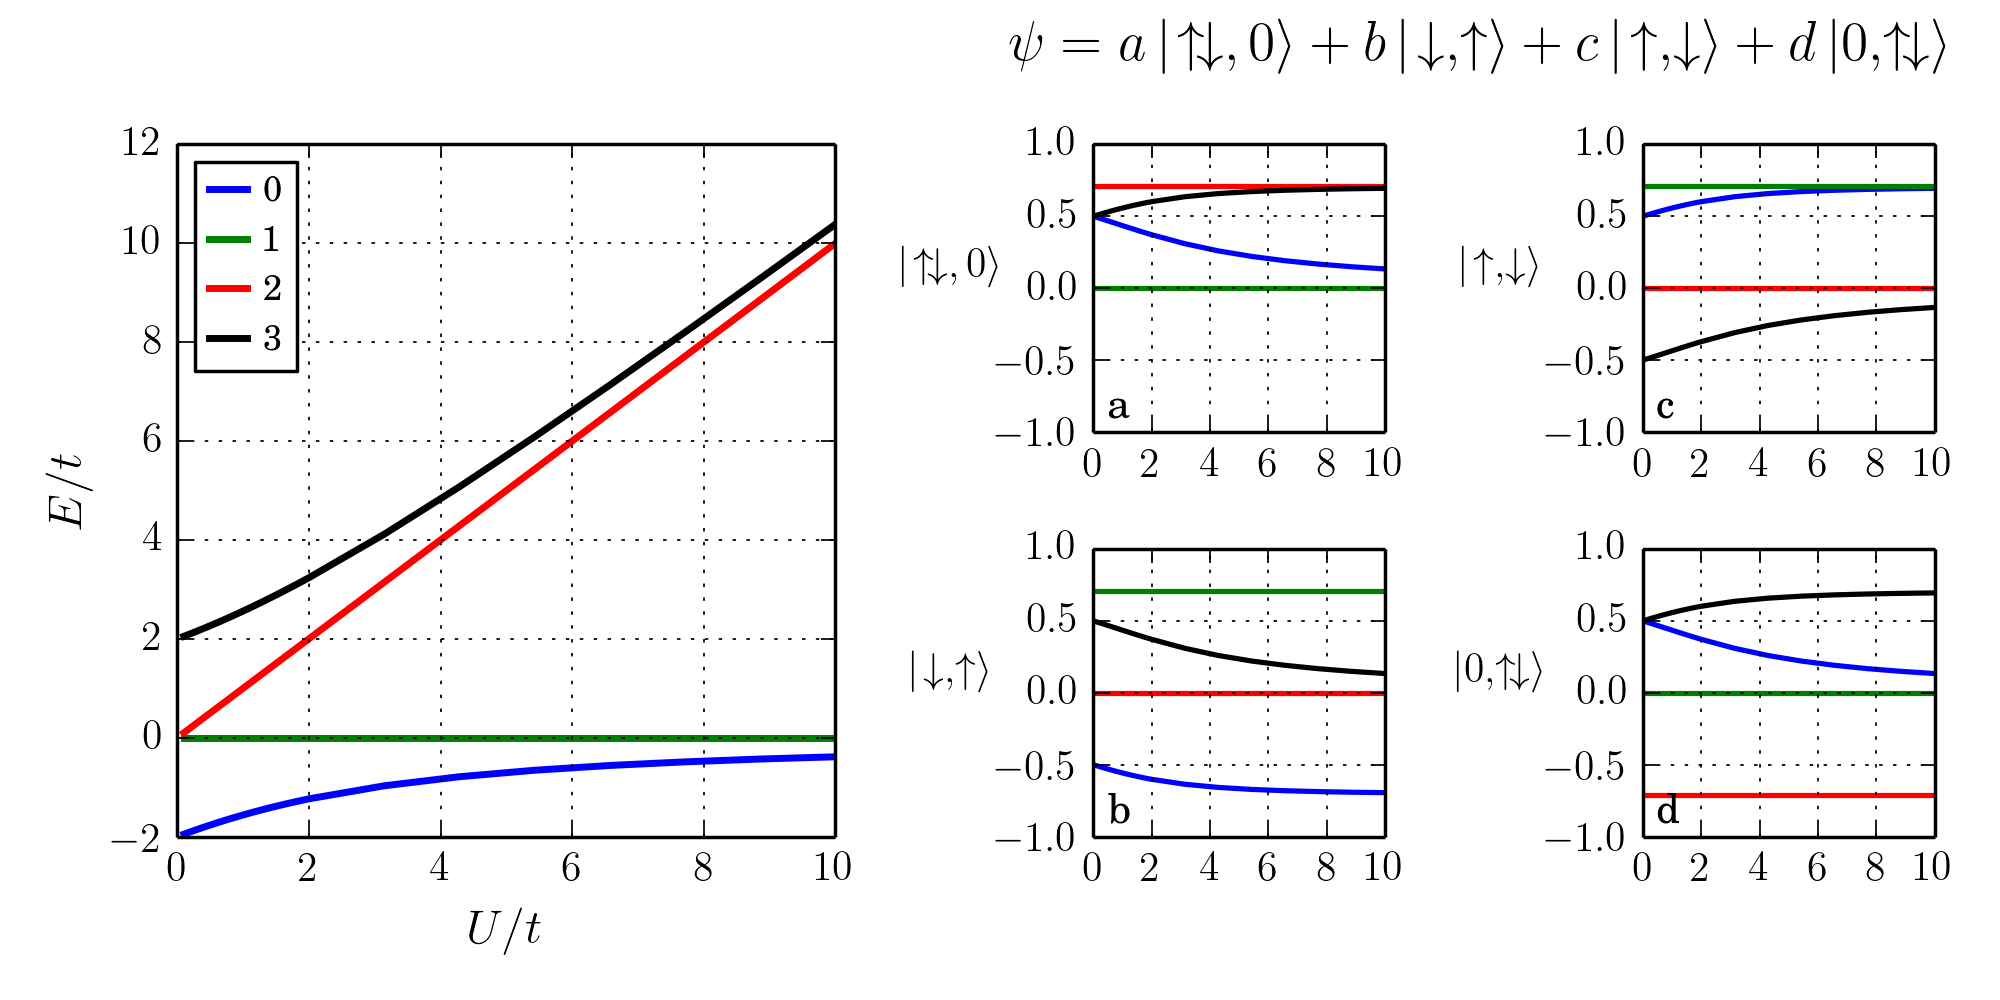
\includegraphics[width=0.8\textwidth]{figures/Ut_eigenvalues_2site.png}
\caption{Exact diagonalization solution for the Hubbard hamiltonian,
Eq.~\ref{eq:Hubbard-U-secondquant}, at half-filling.  Notice that the basis
states used are second quantized staes, so they are already antisymmetrized.
For large $U$ the ground state wavefunction is approximately $\psi =
\frac{1}{\sqrt{2}} (|\spup,\spdn\rangle - |\spdn,\spup\rangle )$.  This state
cannot be written as a Slater determinant because it is an entangled
state.  For a large number of particles the massive enntanglement in the ground
state is what makes strongly correlated systems hard to deal with.
}\label{fig:exactdiag_2site}
\end{figure}

The region in the plot called \textbf{band upper half + $U$} represents the
energy levels in the upper half of the lowest band shifted up by the
interactions.  Of course, this simple picture is not correct in the interacting
many-body system but it provides a good representation of what is going on.  The
separation $U$ between the band lower half and the band upper half can be used
as a measure of the Mott gap. 


\paragraph{First excited band.}  This region is simply bounded by the lowest
and highest energies in the first excited band.  For this band we do not apply
shifts due to interactions.   This band is primarily shown so that, at a
glance, one can asses whether or not the system is in the single band Hubbard
regime.  

\paragraph{Global chemical potential.}  Denoted by $\mu_{0}$. A fixed global
chemical potential is set across the cloud.  The local chemical potential is
obtained by looking at the separation between $\mu_{0}$ and the local zero of
energy.   We remind the reader that the local zero of energy is the point at
the center of the lowest band, i.e. the upper boundary of the blue shaded
region.

\paragraph{Evaporation threshold.}  This is the energy required to escape along
one of the lattice beams.  It is calculated by looking at the profile of the
lowest energy level along the 100 direction and finding its maximum.    In most
cases the maximum will be at infinity, but for $\awaist < 1 $ the lowest energy
profile along 100 can have a local maximum.   In such cases the local maximum
is used. 

\paragraph{Figure of merit for evaporative cooling in the lattice
($\eta_{F}$).} 

When evaporative cooling a thermal gas of atoms, one considers the parameter
$\eta=U_{\text{trap}}/\kb T$, where $T$ is the temperature of the gas, and
$U_{\text{trap}}$ is the energy threshold for a particle leaving the trap (i.e.
the trap depth) measured with respect to the lowest single-particle energy
state.  The evaporation rate is suppressed by a factor $\exp(-\eta)$ where
typically $\eta\sim10$ and, as the gas cools down, the trap depth is reduced to
force further evaporation~\cite{OHara2001}.  

For a deeply degenerate Fermi gas,  $T \ll T_{F}$, the evaporation rate is
given by~\cite{OHara2001}.
\begin{equation}
  \Gamma_{\text{evap}} \propto \gamma_{\text{coll}} \frac{T}{T_{F}} 
  \exp\left[ -   
  \frac{ U_{\text{trap}} - \kb T_{F} }{ \kb T }  \right ] 
\end{equation}
where $\gamma_{\text{coll}}$ is the classical collision rate evaluated at the
Fermi surface.  This can also be written as 
\begin{equation}
  \Gamma_{\text{evap}} \propto \gamma_{\text{coll}} \frac{T}{T_{F}}
  \exp\left[ \frac{1}{T/T_{F}} \right]  
  \exp\left[ -  \frac{1}{T/T_{F}} \left( \frac{U_{\text{trap}}}{\kb T_{F}} \right) \right] 
\end{equation}
We define $ \eta_{F} \equiv U_{\text{trap}}/\kb T_{F}$ and observe that 
\begin{equation}
  \Gamma_{\text{evap}} \propto \gamma_{\text{coll}} \frac{T}{T_{F}}
  \exp\left[ -  \frac{\eta_{F} - 1 }{ T/T_{F} } \right]
\end{equation}
We see that for a given value of $T/T_{F}$, the evaporation rate depends only
on $\eta_{F}$.    The effective $\eta$ factor which determines the exponential
suppression of the evaporation due to the trap depth is given by
\begin{equation}
 \exp(-\eta_{\text{eff}})  = 
  \frac{T}{T_{F}} \exp\left[- \frac{\eta_{F} - 1 }{T/T_{F} } \right]
\end{equation}
Besides the Boltzmann exponential suppression, the evaporation rate is
additionally suppressed by a factor $T/T_{F}$ due to Pauli blocking of one of
the final states of a collision, which occurs for $T\ll
T_{F}$~\cite{OHara2001}.    For a value of $T/T_{F}=0.1$ to get
$\eta_{\text{eff}}=10$ we need $\eta_{F} = 1.77 $ 

\paragraph{Lattice potential} This line shows a representation of the
modulation produced by the lattice potential.   The period of the modulations
shown is arbitrary and only for illustration purposes.  A thin line is also
plotted showing the envelope of the lattice potential.  

 
\paragraph{Trap profiles of thermodynamic quantities.}  The smaller plot on the
top left corner on Fig.~\ref{fig:HTSE_LDA_harmonic} shows the trap profiles of
the thermodynamic quantities.   It includes the density ($d$), double occupancy
($d$), entropy per lattice site ($s_{L}$) and entropy per particle ($s_{N}$).
The entropy per particle is shown on the right side axis.

\paragraph{Overall values of the thermodynamic quantities.} The labels on the
top left of the the smaller plot indicate the overall trap values of the
thermodynamic quantities that can be obtained by integrating the local values
across the volume of the trap. 

Now that we have explained the relevant profiles and quantities that can be
obtained from the LDA we will use it to get some insight on the idea of entropy
redistribution and  the possibility of evaporative cooling in the lattice.  In
the next section we will show how to quantify the entropy capacity of a certain
trap configuration.   After that we will explore the parameter space and will
study the compromise between $\eta_{F}$ (the figure of merit for evaporative
cooling) and the entropy capacity,  keeping in mind that the experiment is
constrained by the number of atoms that can be cooled down to $T/T_{F} < 0.05 $
in the harmonic trap. 


\subsection{ Entropy redistribution }

In the quest for producing an antiferromagnetically (AFM) ordered state with
cold atoms, the entropy per particle, $S/N$,  is an important metric.  It
determines the number of quantum states that are accessible to each atom.  At
half-filling there is an average of one-particle per site\footnote{Notice that
half-filling corresponds to $n=1$, for this reason sometimes the terms
half-filling, unit filling, and unit density are used interchangeably.  Here we
will restrict the terminology to half-filling or we will write explicitly $n=1$
to avoid confusion.}.  If the temperature of the system is high, $T\gg U$,
there is an equal probability for a site to be empty, singly or doubly
occupied.  If  the site is  singly occupied, the spin there could be up or
down, so at high temperatures there are a total of four ( $|0\rangle,
|\spup\rangle, |\spdn\rangle, |\dbl\rangle$ ) equally probable state at each
lattice site, giving an entropy per particle\footnote{Notice that at
half-filling any quantity per particle is the same as per lattice site, since
$n=1$}  equal to $s/\kb=\ln 4 = 1.38$.

When the temperature is $T\ll U$, double occupancies and vacancies are suppressed
and the system enters the Mott insulating state.  In this case the probability
of having empty sites or doubly occupied sites goes to zero.   At each site, a
particle can still  be spin-up or spin-down with equal probability, so the
entropy per particle becomes $s/\kb = \ln 2 = 0.69 $.   

As the temperature of the system goes below the N\'{e}el temperature, the spin
of the atoms becomes strongly determined by their position in the lattice,  as
they start to order antiferromagnetically.  At zero temperature each site has
only one possible quantum state (spin-up or spin-down depending on the lattice
site) and the entropy per particle goes to zero.   

\begin{figure}
        \centering
        \begin{subfigure}[b]{0.48\textwidth}
                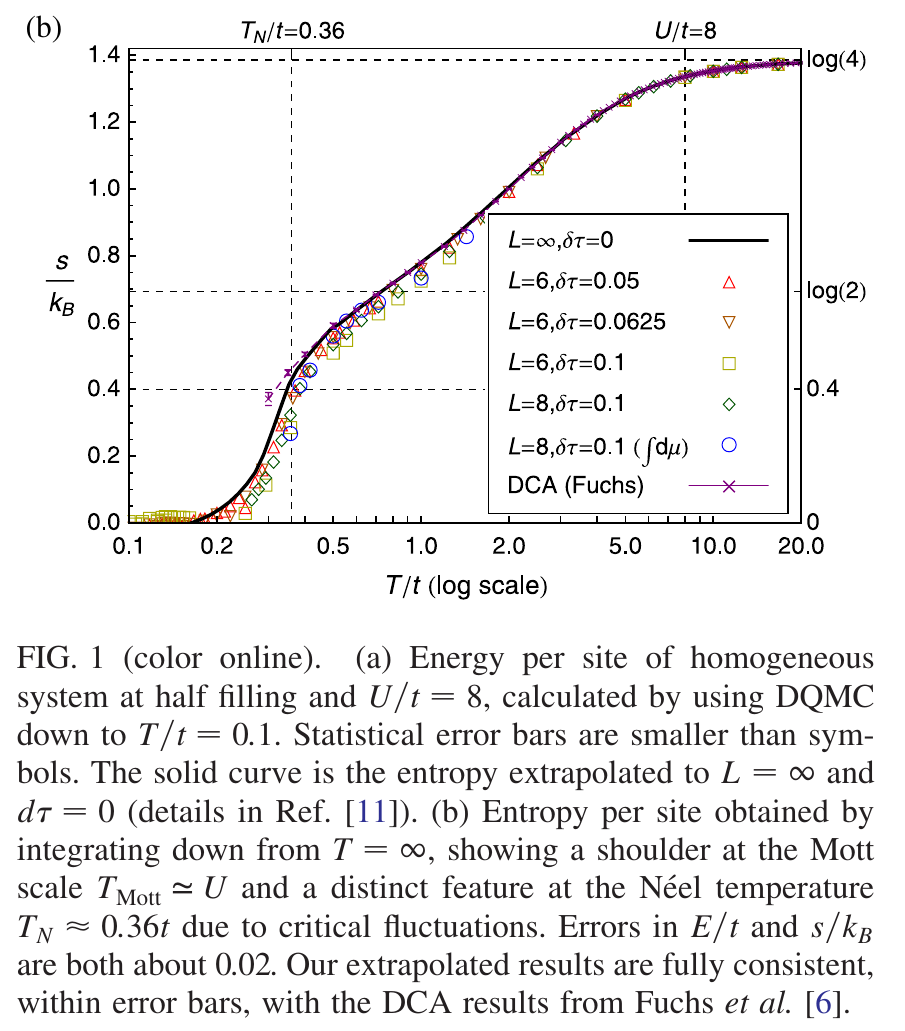
\includegraphics[width=\textwidth]{figures/paiva_entropy.png}
                \caption{Paiva~\cite{Paiva2011}}
                \label{fig:paiva-entropy3D}
        \end{subfigure}
        ~ %add desired spacing between images, e. g. ~, \quad, \qquad etc.
          %(or a blank line to force the subfigure onto a new line)
        \begin{subfigure}[b]{0.48\textwidth}
                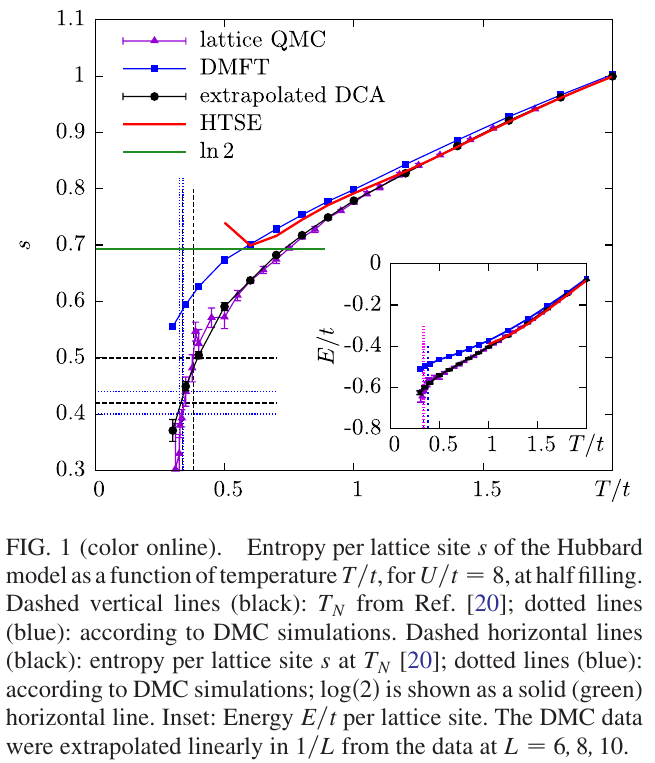
\includegraphics[width=\textwidth]{figures/fuchs_entropy.png}
                \caption{Fuchs~\cite{Fuchs2011}}
                \label{fig:fuchs-entropy3D}
        \end{subfigure}%
        \caption{Calculations of entropy per lattice site versus temperature at half filling.}\label{fig:entropy-Fuchs-Paiva}
\end{figure}
For a homogeneous 3D lattice, at the N\'{e}el temperature $T_{N}=0.36t$, the
entropy per particle is $s=0.4\,\kb$.  As the temperature starts dropping below
$T_{N}$ the entropy approaches zero very quickly in what is referred to as the
AFM transition (AFM stands for antiferromagnetic order).  The AFM transition
has been studied theoretically for homogeneous 3D systems using  quantum
Monte Carlo (QMC)~\cite{Paiva2011} and the dynamical cluster approximation
(DCA)~\cite{Fuchs2011}.  The results from these two approaches are shown in
Figs.~\ref{fig:paiva-entropy3D},\ref{fig:fuchs-entropy3D}.

The theoretical calculations shown correspond to a homogeneous system, but in
practice  one has samples with a finite number of atoms so one is forced to
confine them in order to reach half-filling.   Since the confinement is
typically harmonic (as opposed to a well with hard walls), the density decays
as a function of distance to the center.   The inhomogeneity in the density
leads to the concept of entropy redistribution.  As a consequence, the overall
entropy per particle  necessary to achieve a N\'{e}el state can be higher in a
trapped system that in the homogeneous case~\cite{Paiva2011}. 


\subsubsection{High temperature series expansion for the Hubbard model}

The high temperature series expansion (HTSE) to second
order~\cite{Henderson1992,Jordens2010} allows us to visualize the properties of
the Hubbard model.  It works well to capture the properties of the Mott
insulating state, however it fails below temperatures of $T/t~1.8$, so the AFM
state is beyond its reach. 

The signatures of the Mott insulating states can be seen in the HTSE solutions
shown in Fig.~\ref{fig:HTSEhomogeneous}, namely: 
\begin{itemize} 
\item The density as function of chemical potential has a
plateau at $n=1$, Fig.\ref{fig:HTSEhomogeneousA}.  
\item The double occupancy
is suppressed for lower temperatures, Fig.~\ref{fig:HTSEhomogeneousB}.  
\item
The density fluctuations are suppressed, Fig.~\ref{fig:HTSEhomogeneousC}.
\item The entropy per site as a function of filling has a dip at $n=1$,
Fig.~\ref{fig:HTSEhomogeneousD}. 
\end{itemize} 
\begin{figure}
        \centering
        \begin{subfigure}[b]{0.49\textwidth}
                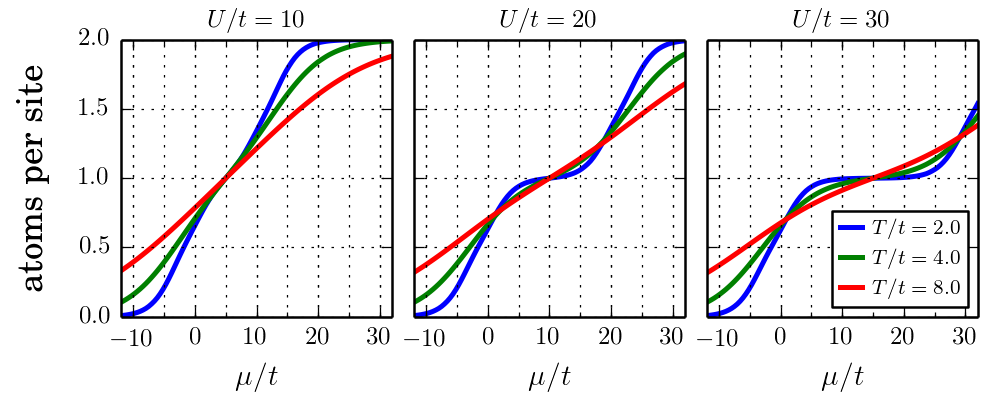
\includegraphics[width=\textwidth]{figures/HTSE_density_U.png}
                \caption{Density}
\label{fig:HTSEhomogeneousA}
        \end{subfigure}%
          %add desired spacing between images, e. g. ~, \quad, \qquad etc.
          %(or a blank line to force the subfigure onto a new line)
        ~
        \begin{subfigure}[b]{0.49\textwidth}
                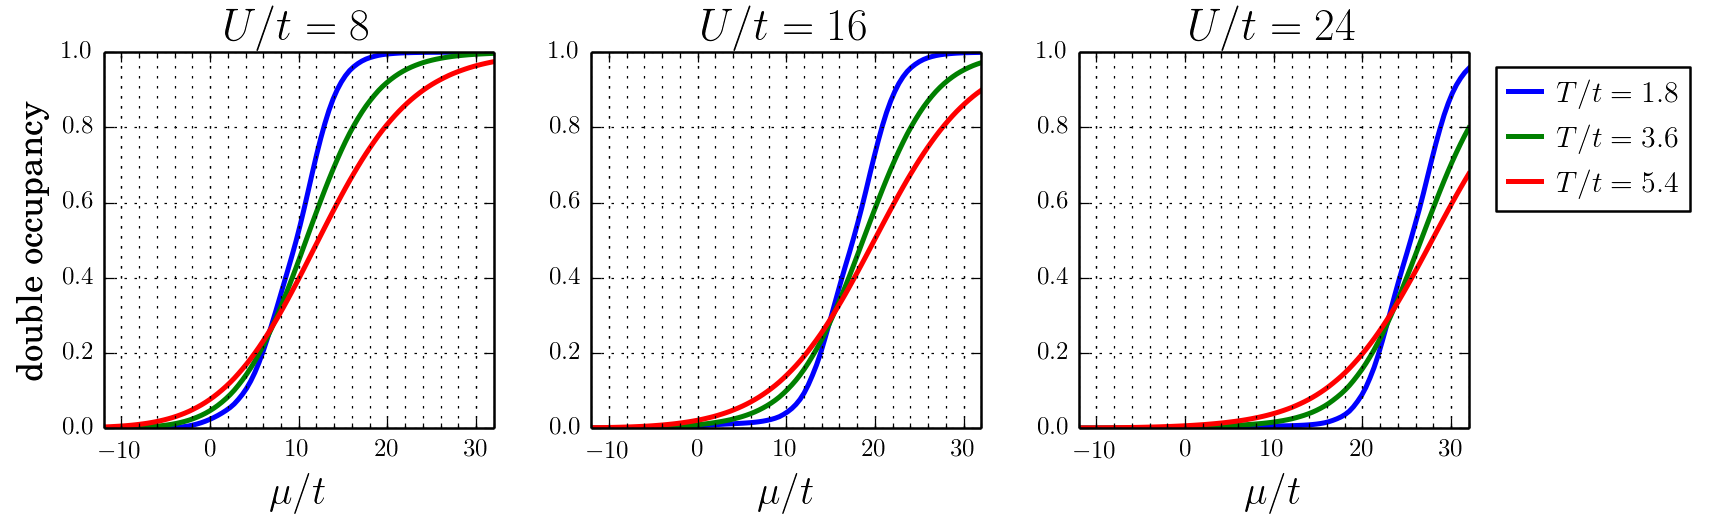
\includegraphics[width=\textwidth]{figures/HTSE_doublons_U.png}
                \caption{Double occupancy}
\label{fig:HTSEhomogeneousB}
        \end{subfigure}
 
        \begin{subfigure}[b]{0.49\textwidth}
                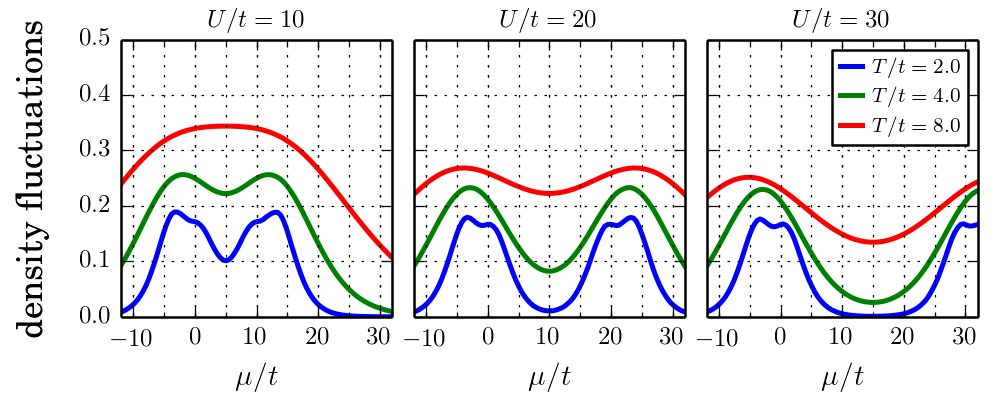
\includegraphics[width=\textwidth]{figures/HTSE_densfluc_U.png}
                \caption{Density fluctuations}
\label{fig:HTSEhomogeneousC}
        \end{subfigure}
        ~
        \begin{subfigure}[b]{0.49\textwidth}
                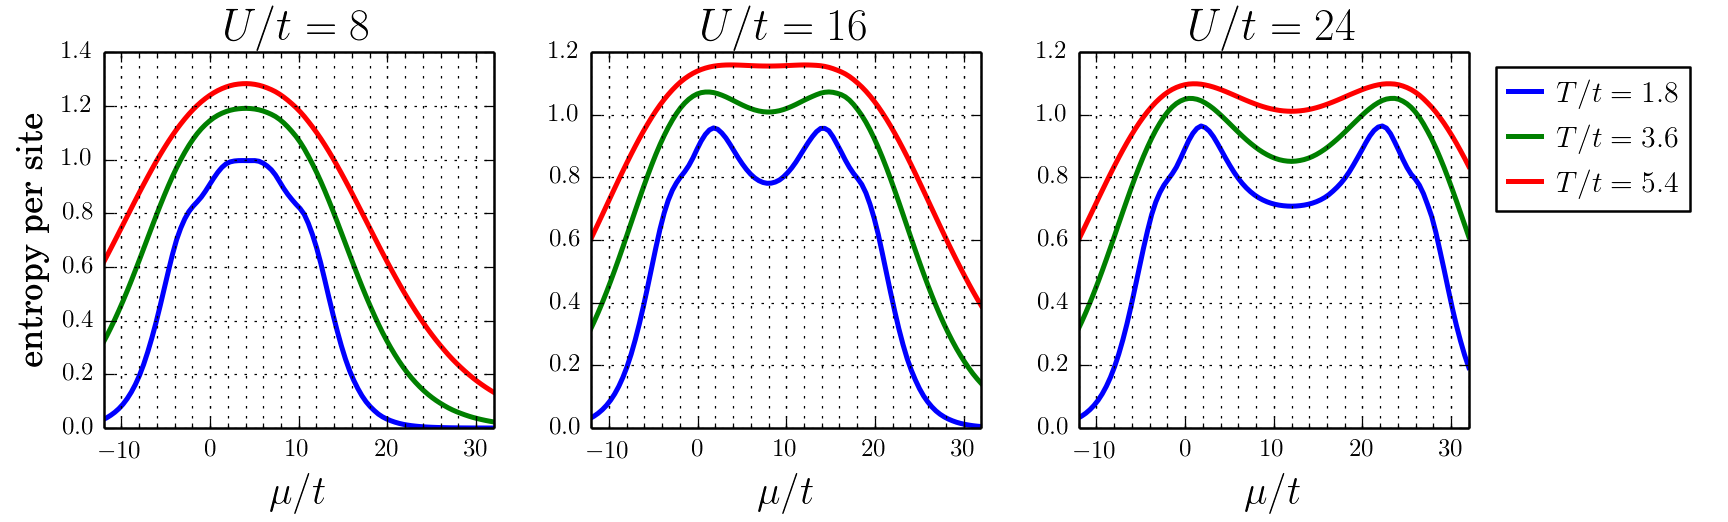
\includegraphics[width=\textwidth]{figures/HTSE_entropy_U.png}
                \caption{Entropy per lattice site}
\label{fig:HTSEhomogeneousD}
        \end{subfigure}
        \caption{Thermodynamic quantities as a function of chemical potential calculated using the HTSE.}
\label{fig:HTSEhomogeneous}
\end{figure}


\subsubsection{Entropy per particle}  

\begin{figure}
    \centering
    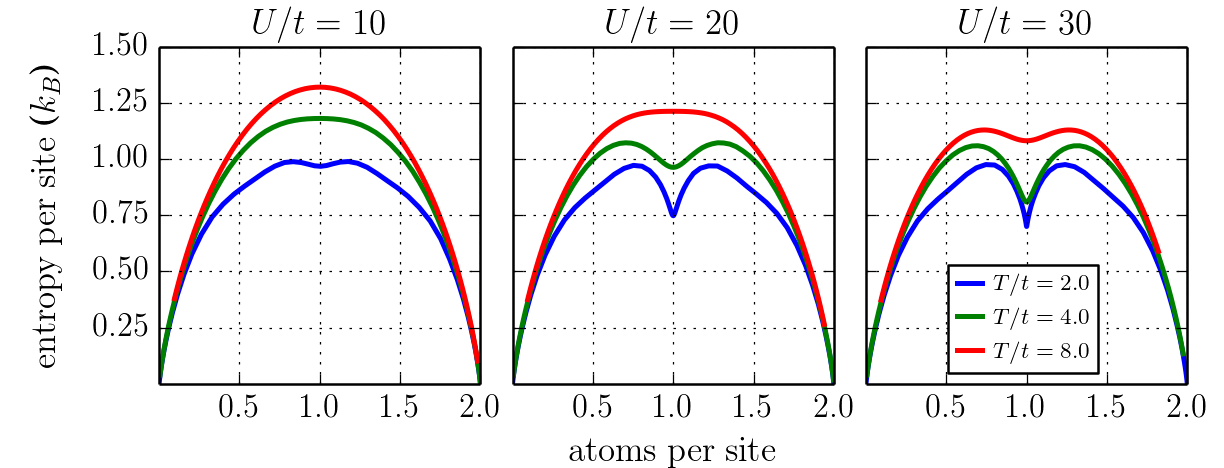
\includegraphics[width=0.65\textwidth]{figures/HTSE_EntropyPerSite_U.png}
    \caption{Entropy per lattice site versus density.}\label{fig:HTSE_spersite}
\end{figure}
The HTSE gives us the result for the entropy per lattice site, which we can
plot versus the density, as shown in Fig.~\ref{fig:HTSE_spersite}  The
interesting result arises if we divide the entropy per lattice site by the
density, in order to obtain the entropy per particle.  This is shown in
Fig.~\ref{fig:HTSE_sperparticle}. 
\begin{figure}
    \centering
    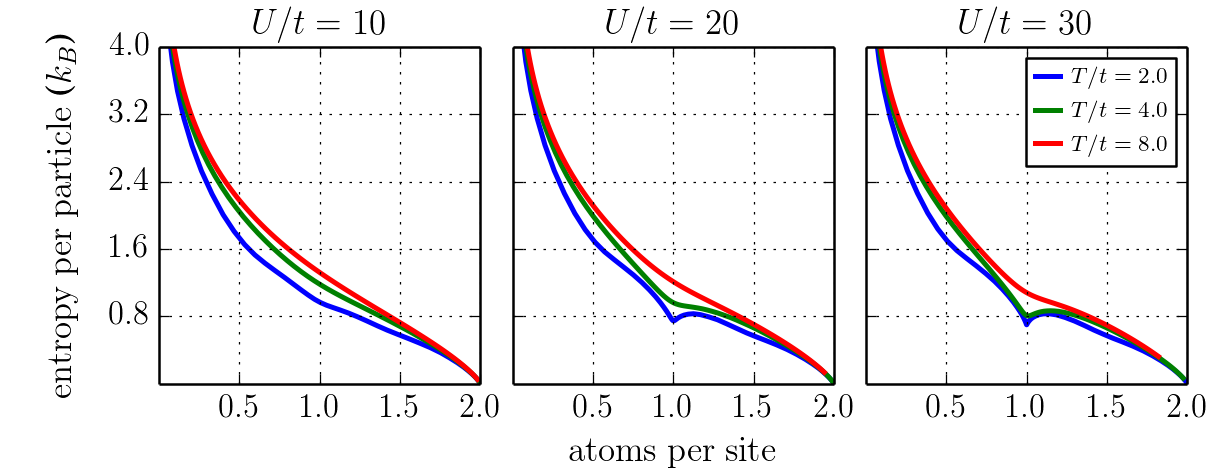
\includegraphics[width=0.65\textwidth]{figures/HTSE_EntropyPerParticle_U.png}
    \caption{Entropy per particle versus density.}\label{fig:HTSE_sperparticle}
\end{figure}
It is seen there that the entropy per particle rises significantly for lower
filling values, and most importantly that the value of the entropy per particle
at low filling \textbf{does not} depend strongly on temperature or interaction
strength.   

In a finite trapped system which inevitably has a shell with density $n<1$ , a
large part of the total entropy of the system is carried by particles in the
shell.  This allows the core to be at an effectively lower entropy per
particle.  At a lower entropy per particle the core can enter the AFM state
even if the overall value of $S/N$ for the entire trap 	is larger than the
N\'{e}el entropy of the homogeneous system,  $s_{\text{N\'{e}el}} = 0.4
k_{\text{B}}$.   A QMC calculation shows that  $S/N=0.65k_{\text{B}}$ may be
low enough to reach an AFM state at the core of the sample.   If the sample is
loaded adiabatically from a harmonic trap into the lattice this entropy per
particle corresponds to $T/T_{F} = 0.06$ in the harmonic trap. 

\subsubsection{ Comparing  entropy redistribution scenarios} 

We can consider compensated lattice setups with different beam waist ratios
$\awaist$ and different compensation values and determine which setup offers
the best scenario for entropy redistribution.  There are two approaches to do
this. One can realize the LDA at a fixed value of $S/N$, find out the resulting
temperature of the sample and compare the different scenarios.   Alternaetively
one can realize the LDA at a fixed temperature and compare the values of $S/N$
for different scenarios.   

The first method is more closely related to experiments, because ultracold
atoms are isolated systems and the loading of atoms into the lattice should, in
principle, proceed adiabatically.   In this way one can see for different
setups how will the system be adiabatically heated or cooled as it is loaded
into the lattice.   Since the entropy is a monotonic function of the
temperature the second approax, which realizes the LDA at fixed temperature and
compares the resulting $S/N$ is also valid.  This approach is easier to
implement in the computer code, since the solution to the HTSE is obtained from
the grand canonical partition function, which assumes the system is at fixed
temperature.  

\section{LDA Results}

  
\subsection{ Optimization of the evaporation figure of merit  } 

We run the LDA for different values of the lattice and compensation beam
waists.  For each pair of $w_{L}$ and $w_{C}$ values we minimize the value of
$\eta_{F}$  by adjusting the compensation depth $g_{0}$.   The following
constraints are enforced:
\begin{itemize}
  \item The global chemical potential is set at $U/2$ to enforce $n=1$ at the center of the sample.
  \item The lowest band is required to have a positive curvature at the origin.
\item The resulting density profile is required to decrease monotonically as a
function of distance from the center.  
\item The chemical potential is
restricted to be below the energy required for an atom to move along a beam.
The purpose of this restriction is to avoid having atoms residing along the
lattice beams outisde of the beam intersection region.  Since we do the LDA at
a non-zero temperature, this restriction is implemented as 
\[ \mu + T < E_{\text{th}}
\] where $E_{\text{th}}$  is the energy required for an atom to escape along
the beams.
\end{itemize}

Once the value of the compensation is set to minimize $\eta_{F}$ the system is
defined and we can look at the number of atoms required to realize it and also
at the value of $S/N$, to assess the capability that the particular
configuration has to redistribute the entropy.   The results of this
optimization are shown in Figs.~\ref{fig:optimize_etaF}
and~\ref{fig:optimize_etaF_cold}.
\begin{figure}
    \centering
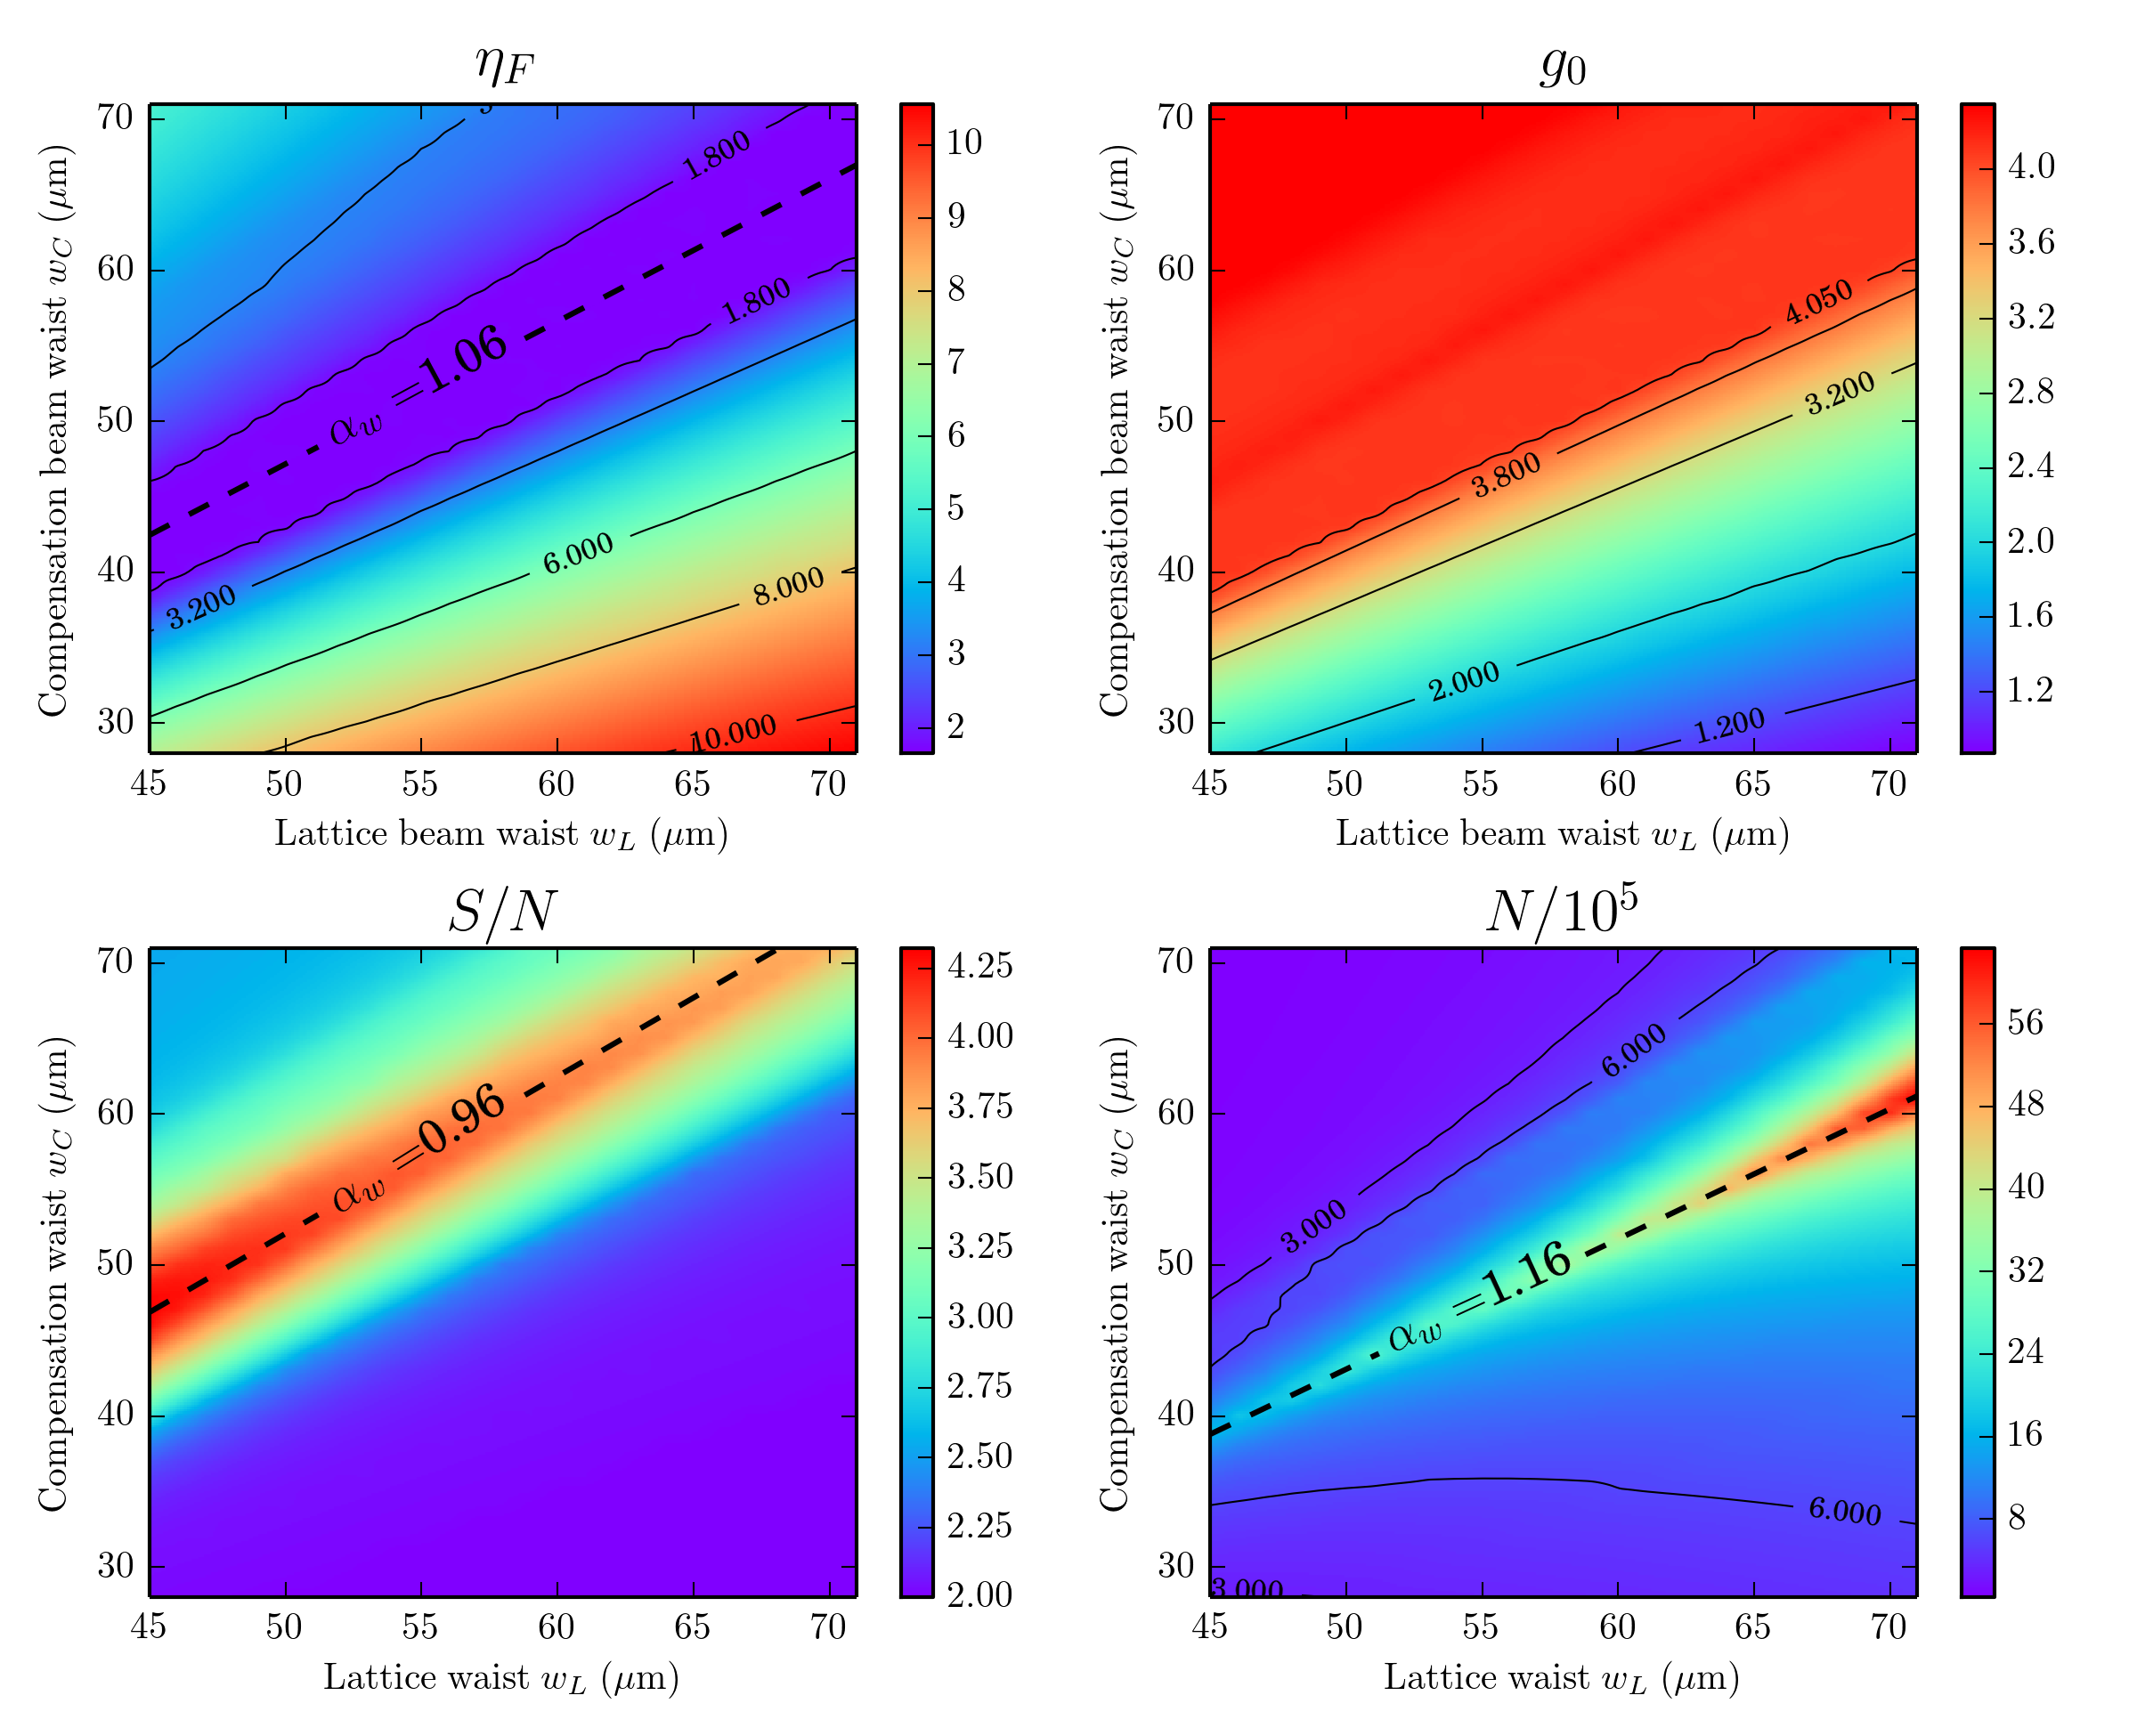
\includegraphics[width=0.65\textwidth]{figures_hubbard-lda/etaF-wIRwGR.png}
\caption{LDA results for the optimization of the evaporation figure of merit
$\eta_{F}$. The calculation was performed at a temperature of $T=0.4\,E_{R}$,
which for a 7\,$E_{R}$ lattice corresponds to $T=10.1t$ at the center.  The
interactions are set at 650\,$a_{0}$ which is $U/t=24.8$ at the center. }
    \label{fig:optimize_etaF}
\end{figure}

\begin{figure}
    \centering
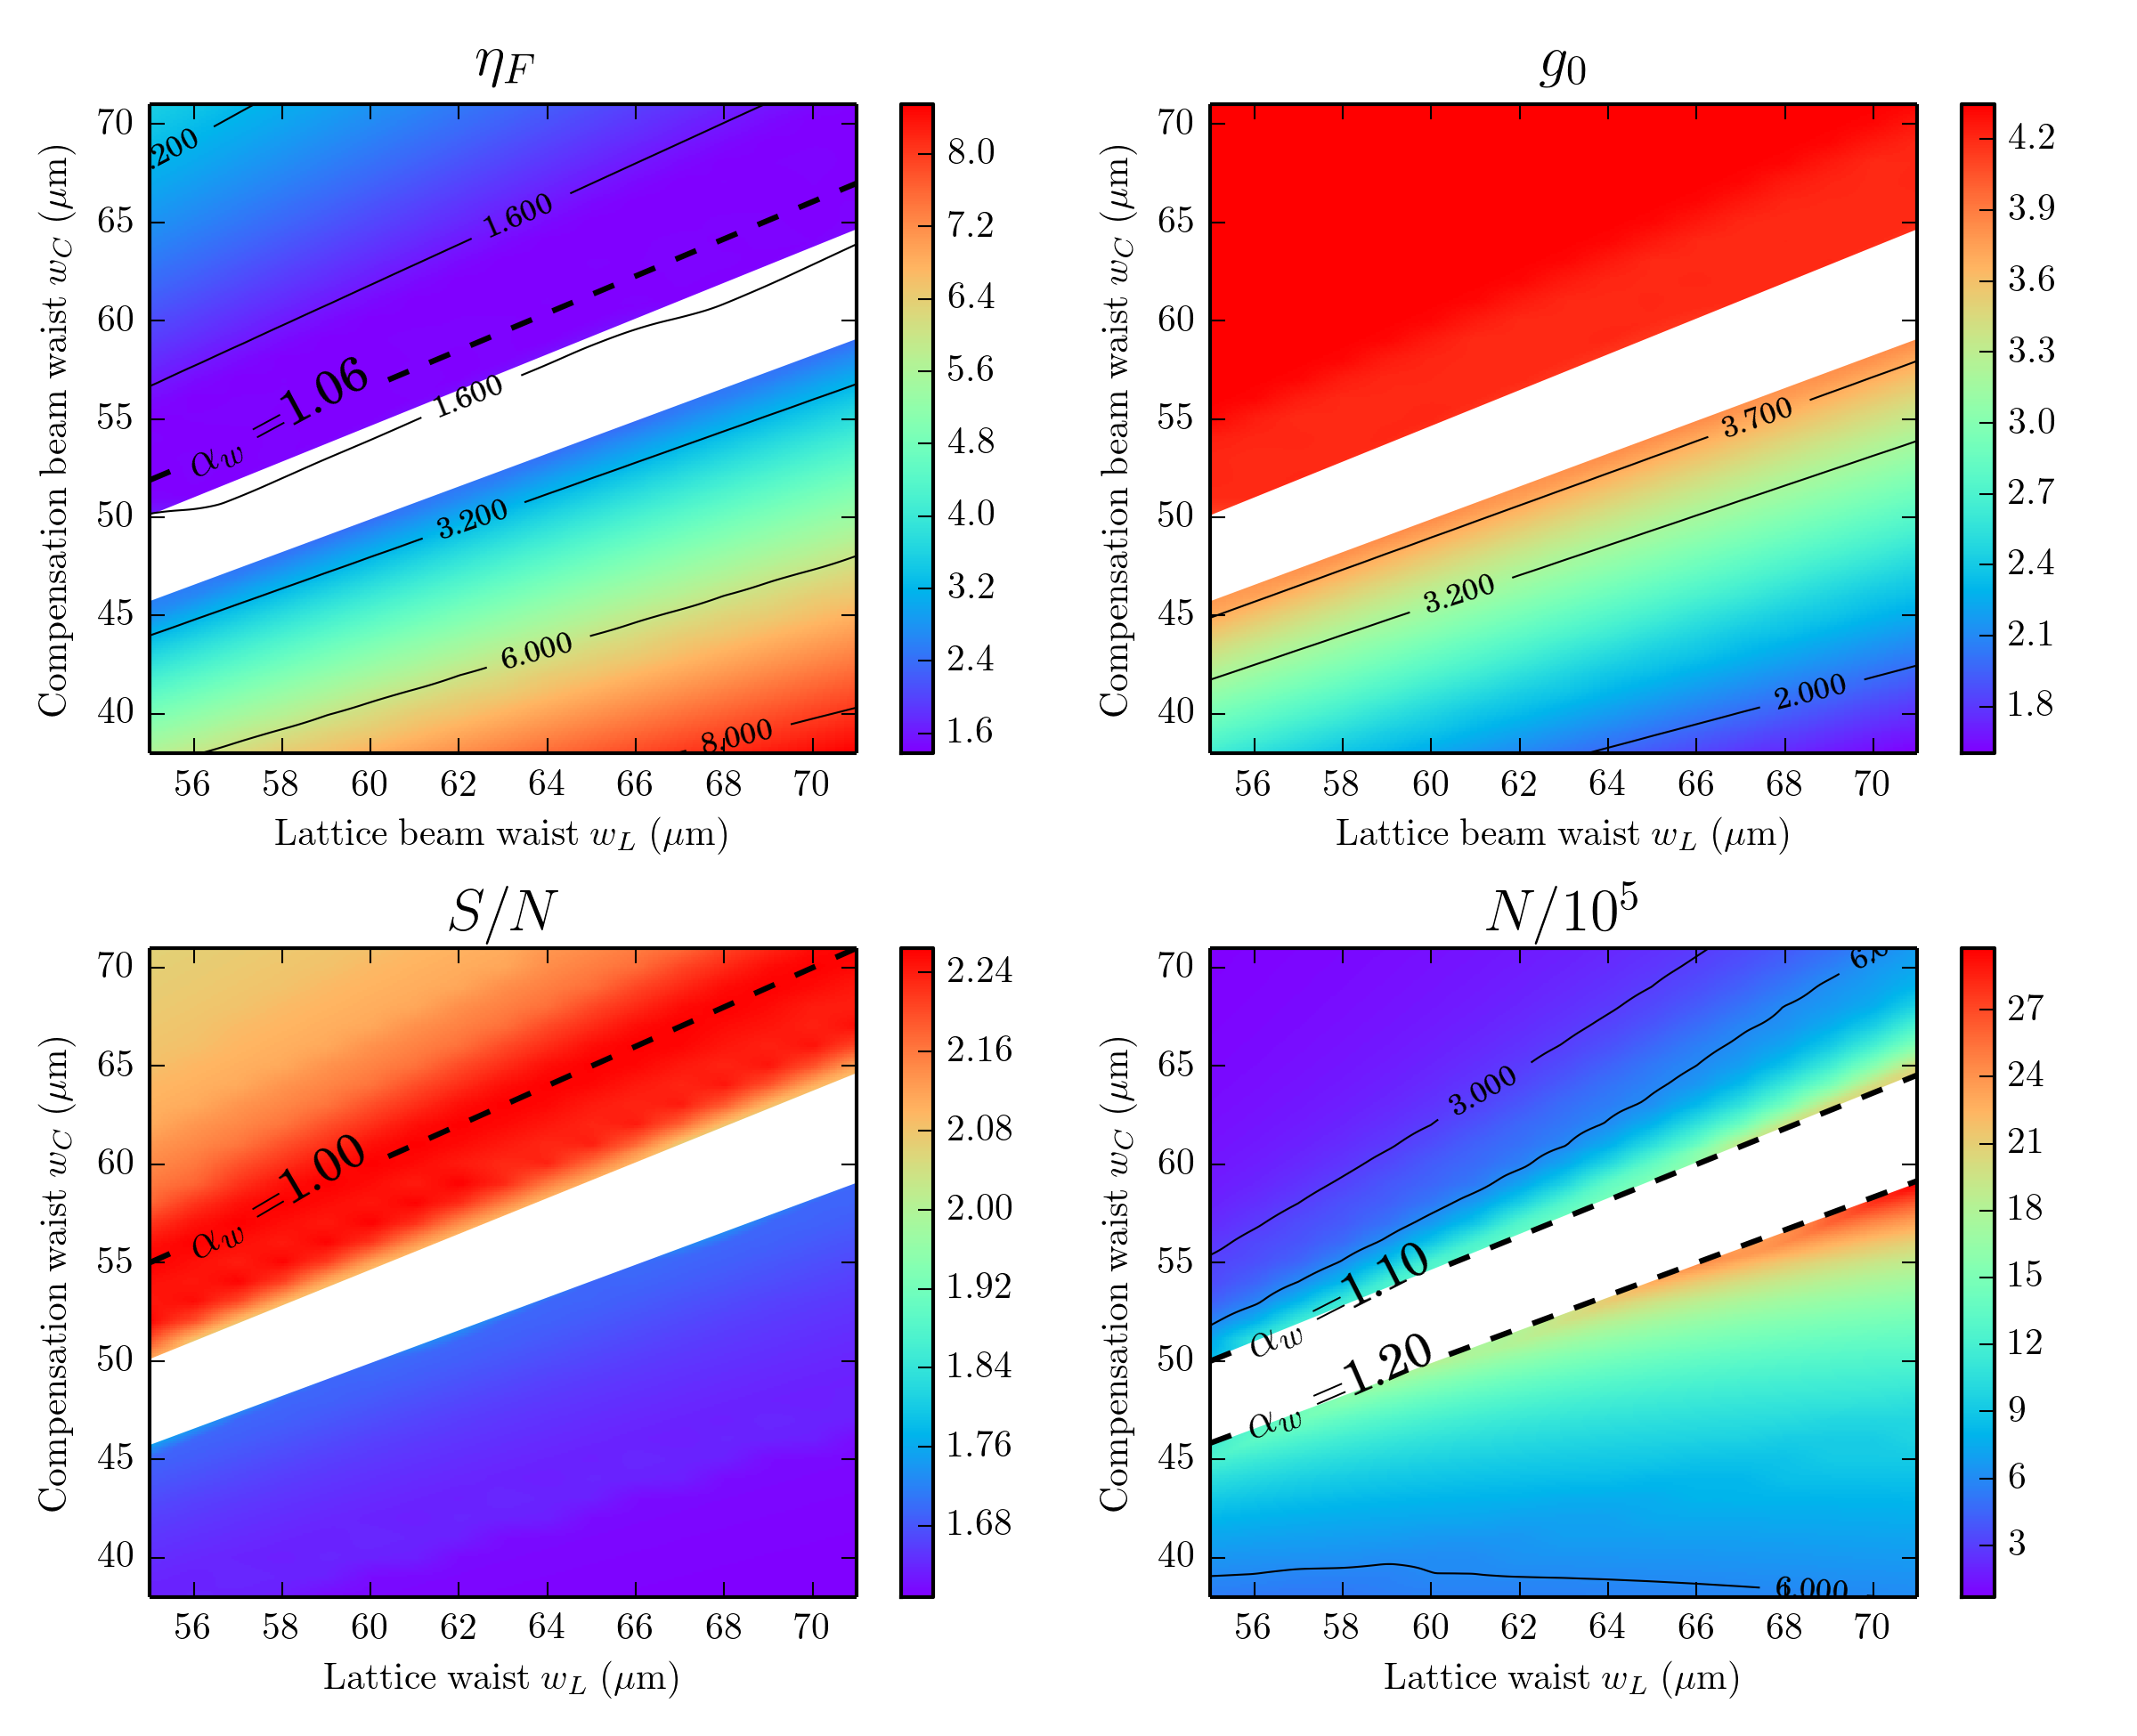
\includegraphics[width=0.65\textwidth]{figures_hubbard-lda/etaF-wIRwGR_cold.png}
\caption{LDA results for the optimization of the evaporation figure of merit
$\eta_{F}$. The calculation was performed at a temperature of $T=0.2\,E_{R}$,
which for a 7\,$E_{R}$ lattice corresponds to $T=5.1t$ at the center. In order
to achieve lower temperatures we did not cover the region with optimal
compensation from $\awaist=1.10$ to 1.20.   At an optimal compensation the
radius of the sample is a large fraction of the beam waist and the value of
$T/t$ at the edge of the cloed is out of reach for the HTSE.  The interactions
are set at 650\,$a_{0}$ which is $U/t=24.8$ at the center. }
    \label{fig:optimize_etaF_cold}
\end{figure}

\paragraph{Observations.} 

\begin{itemize} 
\item For $\awaist<1.16$ the value of green compensation is fixed at
$g_{0}\approx 4.1\,E_{R}$.   This means that for $\awaist < 1.16$ the potential
can always be compensated such that the chemical potential nearly gets to the
energy required to escape along a beam.   For $\awaist \ll 1.16$  the lowest
energy along a beam direction (say 100) will have a local maximum. Based on our
constraints we restrict the compensation such that the chemical potential does
not reach the assymptotic energy value along a beam.   $\eta_{F}$ will then
become larger because it is measured with respect to the local maximum
(threshold for evaporation) instead of with respect to the assymptotic energy
value along the beam.  Aside from this aspect, whenever the compensation is
$\approx 4.1\,E_{R}$  we see that $\eta_{F}$ attains the lowest value of
$\approx 1.8$, which is determined by the temperature used in the calculation
(at zero temperature $\eta_{F}=1$ would be achieved).  The temperature we have
used in Fig.~\ref{fig:optimize_etaF} is $T=0.4\,E_{R}$, which for a 7\,$E_{R}$
lattice amounts to $T=10.1t$ at the center.   In
Fig.~\ref{fig:optimize_etaF_cold} results are shown for $T=0.2\,E_{R}$
($T=5.1t$), but a region of the parameter space has to be excluded at this
temperature.  The interactions used  are $a_{s}=650\,a_{0}$, which give
$U/t=24.8$ at the center of the sample. 

A particular aspect of systems with small beam waist is that as one moves away
from the center the lattice depth decays and $t$ gets larger.   For a fixed
value of $T$, then $T/t$ gets smaller as one moves away from the center.  We
set $T/t=10.1$ at the center so that near the edge we are still at $T/t > 1.8$
and the HTSE solution to the Hubbard model is still applicable.   

\item For $\awaist = 1.16$  the sample is flattened optimally with the choice
of compensation that also minimzes $\eta_{F}$.  We obtained nearly the same
result analytically in \S\ref{subsec:compensation}.    Optimal flattening means
that one can accomodate a large amount of atoms in the potential.   If the
atoms are available in the experiment this is a good feature because flattening
also means that the extent of the phase of interest at the core of the sample
will me maximized.  Unfortunately the atom numbers required to reach this
regime are beyond the atom number that we can produce in deeply degenerate
samples in our experiment.  It is tru that using a larger beam waist can most
likely enhance the number of atoms that our experimnent can produce in deeply
degenerate samples, but we expect this number to be less than $8\times10^{5}$
limited by the atoms that can be evaporated in the ODT and the efficiency of
loading them into the dimple potential.   

\item For $\awaist < 1.16$, where $g_{0}$ can be saturated up to $4.1\,E_{R}$
to reach an optimal $\eta_{F}$, we can turn to our second important figure of
merit:  the entropy capacity of the configurtion.   We see that a value of
$\awaist=0.96$ gives an optimal entropy capacity, since it maximizes $S/N$ for
fixed temperature.   

\item For a fixed lattice beam waist we see that we can obtain an optimized
$\eta_{F}$  near 1.8 with a lower atom number if we keep increasing the
compensation beam waist.   This seems counterintuitive at first because the
first thought is that to reach an optimal value of $\eta_{F}$ one must fill up
the lattice beams up some fraction of their waist.    The important point is
that the fraction of the waist depends on compensation.  If the lattice is
flattened optimally then one needs to go far into the lattice beams in order to
get the chemical potential to come close to the threshold.  If the lattice is
just pushed upwards by the compensation but not flattend ( this becomes the
case as $\awaist$ moves below 1.16 ) then the fraction of the waist you need to
fill up to move the chemical potential close to the threshold is much smaller.  
 
In Fig.~\ref{fig:optimize_etaF_hwhm} we show the fraction of the lattice beam
waist that is filled up by the density distribution.  For an optimally
compensated sample at $\awaist=1.16$ the fraction can be as large as 0.72 , but
for $\awaist=0.96$ where the entropy capacity of the system is maximized it can
be as low as 0.47.  

\begin{figure}
    \centering
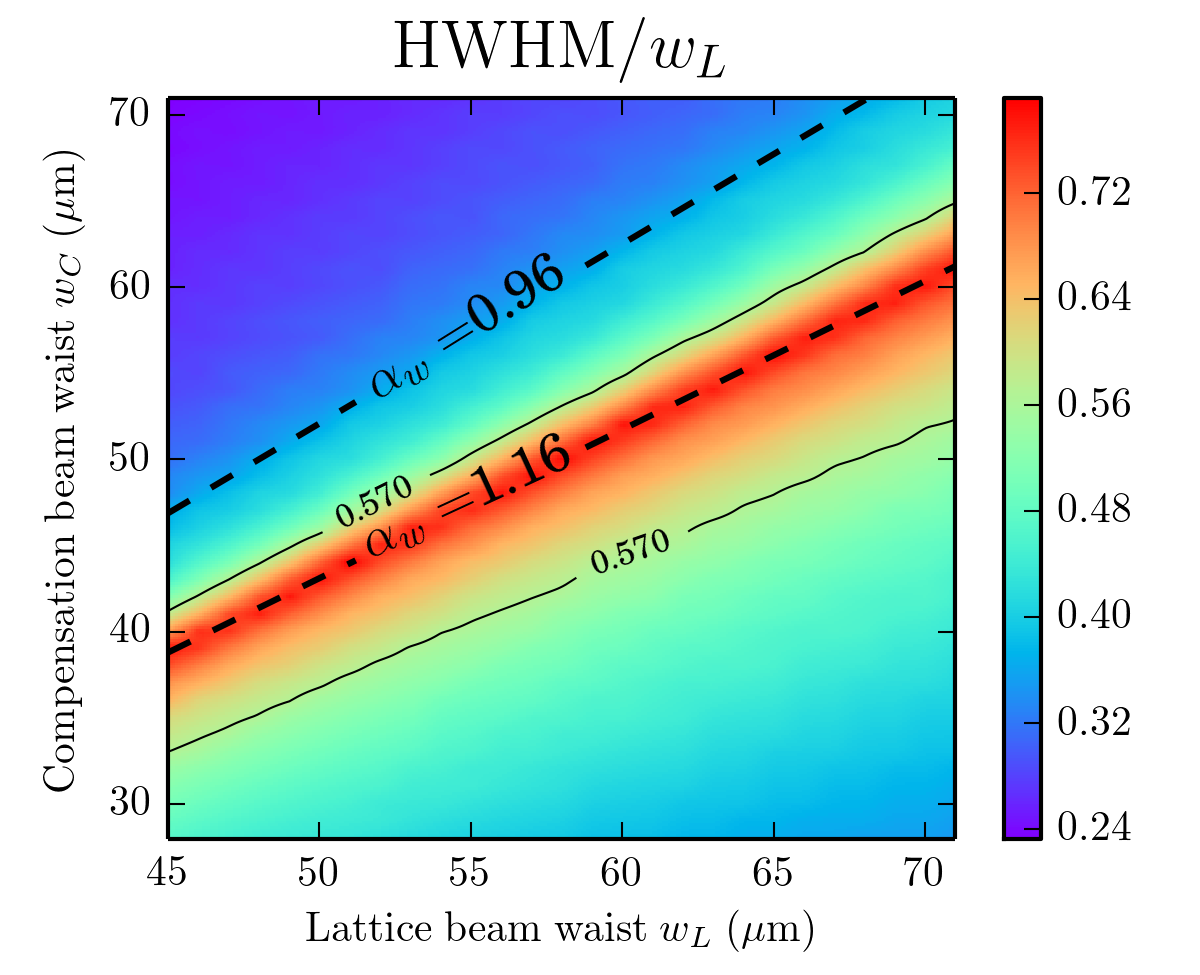
\includegraphics[width=0.4\textwidth]{figures_hubbard-lda/etaF-HWHM-ratio.png}
\caption{For the same LDA calculation shown in Fig.~\ref{fig:optimize_etaF},
this plot shows the ratio of the density profile's half-width at half-max to
the lattice beam waist $w_{L}$.  This shows that for an optimally  flattened
sample, you need to fill up a large fraction of your beams in order to reach a
chemical potential that is favorable for evaporation.   This is why an
optimally flattened sample, $\awaist=1.16$, with  $w_{L}=50\,\mu\mathrm{m}$
requires a similar number of atoms than a sample with $\awaist=1.10$ and
$w_{L}\approx 70\,\mu\mathrm{m}$.}
    \label{fig:optimize_etaF_hwhm}
\end{figure}

\item In conclusion,  if we use a lattice ratio $\awaist=0.96$ we can find a
compensation value that allows us to be at half-filling ($n=1$ at the center),
optimize the evaporation figure of merit ($\eta_{F}$ as close as possible to 1)
and optimize the entropy capacity of the system ($S/N$ maximized for fixed
temperature) all at the same time.   At $\awaist=0.96$ the optimal setup has a
cloud radius that is only $\approx 0.47 w_{L}$.   For a half-filled sample a
crude estimate of the atom number can be obtained as \[  N = \frac{4}{3}\pi
\left( \frac{ r_{\text{cloud}} }{ a } \right)^{3} =  \frac{4}{3}\pi \left(
\frac{ 0.47 w_{L}  }{ a } \right)^{3} \] so a reasonable value of
$N=500,000$  would require a lattice beam waist $w_{L} = 55\,\mu{m}$.   

As was shown in \S\ref{subsec:locking} and Fig.~\ref{fig:lattice_lockB} a
lattice beam waist of 55\,$\mu$m would only allow us to lock a sample of
$500,000$ atoms to a depth of $\approx$10\,$E_{R}$.   In order to satisfy the
requirements of the lattice lock we will need to compromise on one of our
figures of merit. 

\end{itemize}


\subsection{ Lattice locking requirements   } 

Figure~\ref{fig:lattice_lockB} shows us that, with large atom numbers, we need
to have very big lattice beam waists in order to be able to freeze tunneling
and stay in the single band regime.   The analytical result shows that to
succesfully lock a sample up to 30\,$E_{R}$ its radius has to be
$0.32\,w_{L}$.    

We perform an LDA calculation where, for a half-filled sample ($n=1$ at the
center), we vary the value of the green compensation such that the radius of
the sample is  equal to $0.32\,w_{L}$.  The results are shown in
Fig.~\ref{fig:optimize_lock},  which was calculated at a temperature
$T=0.12\,E_{R}$ ($T=3.0t$).    
\begin{figure}
    \centering
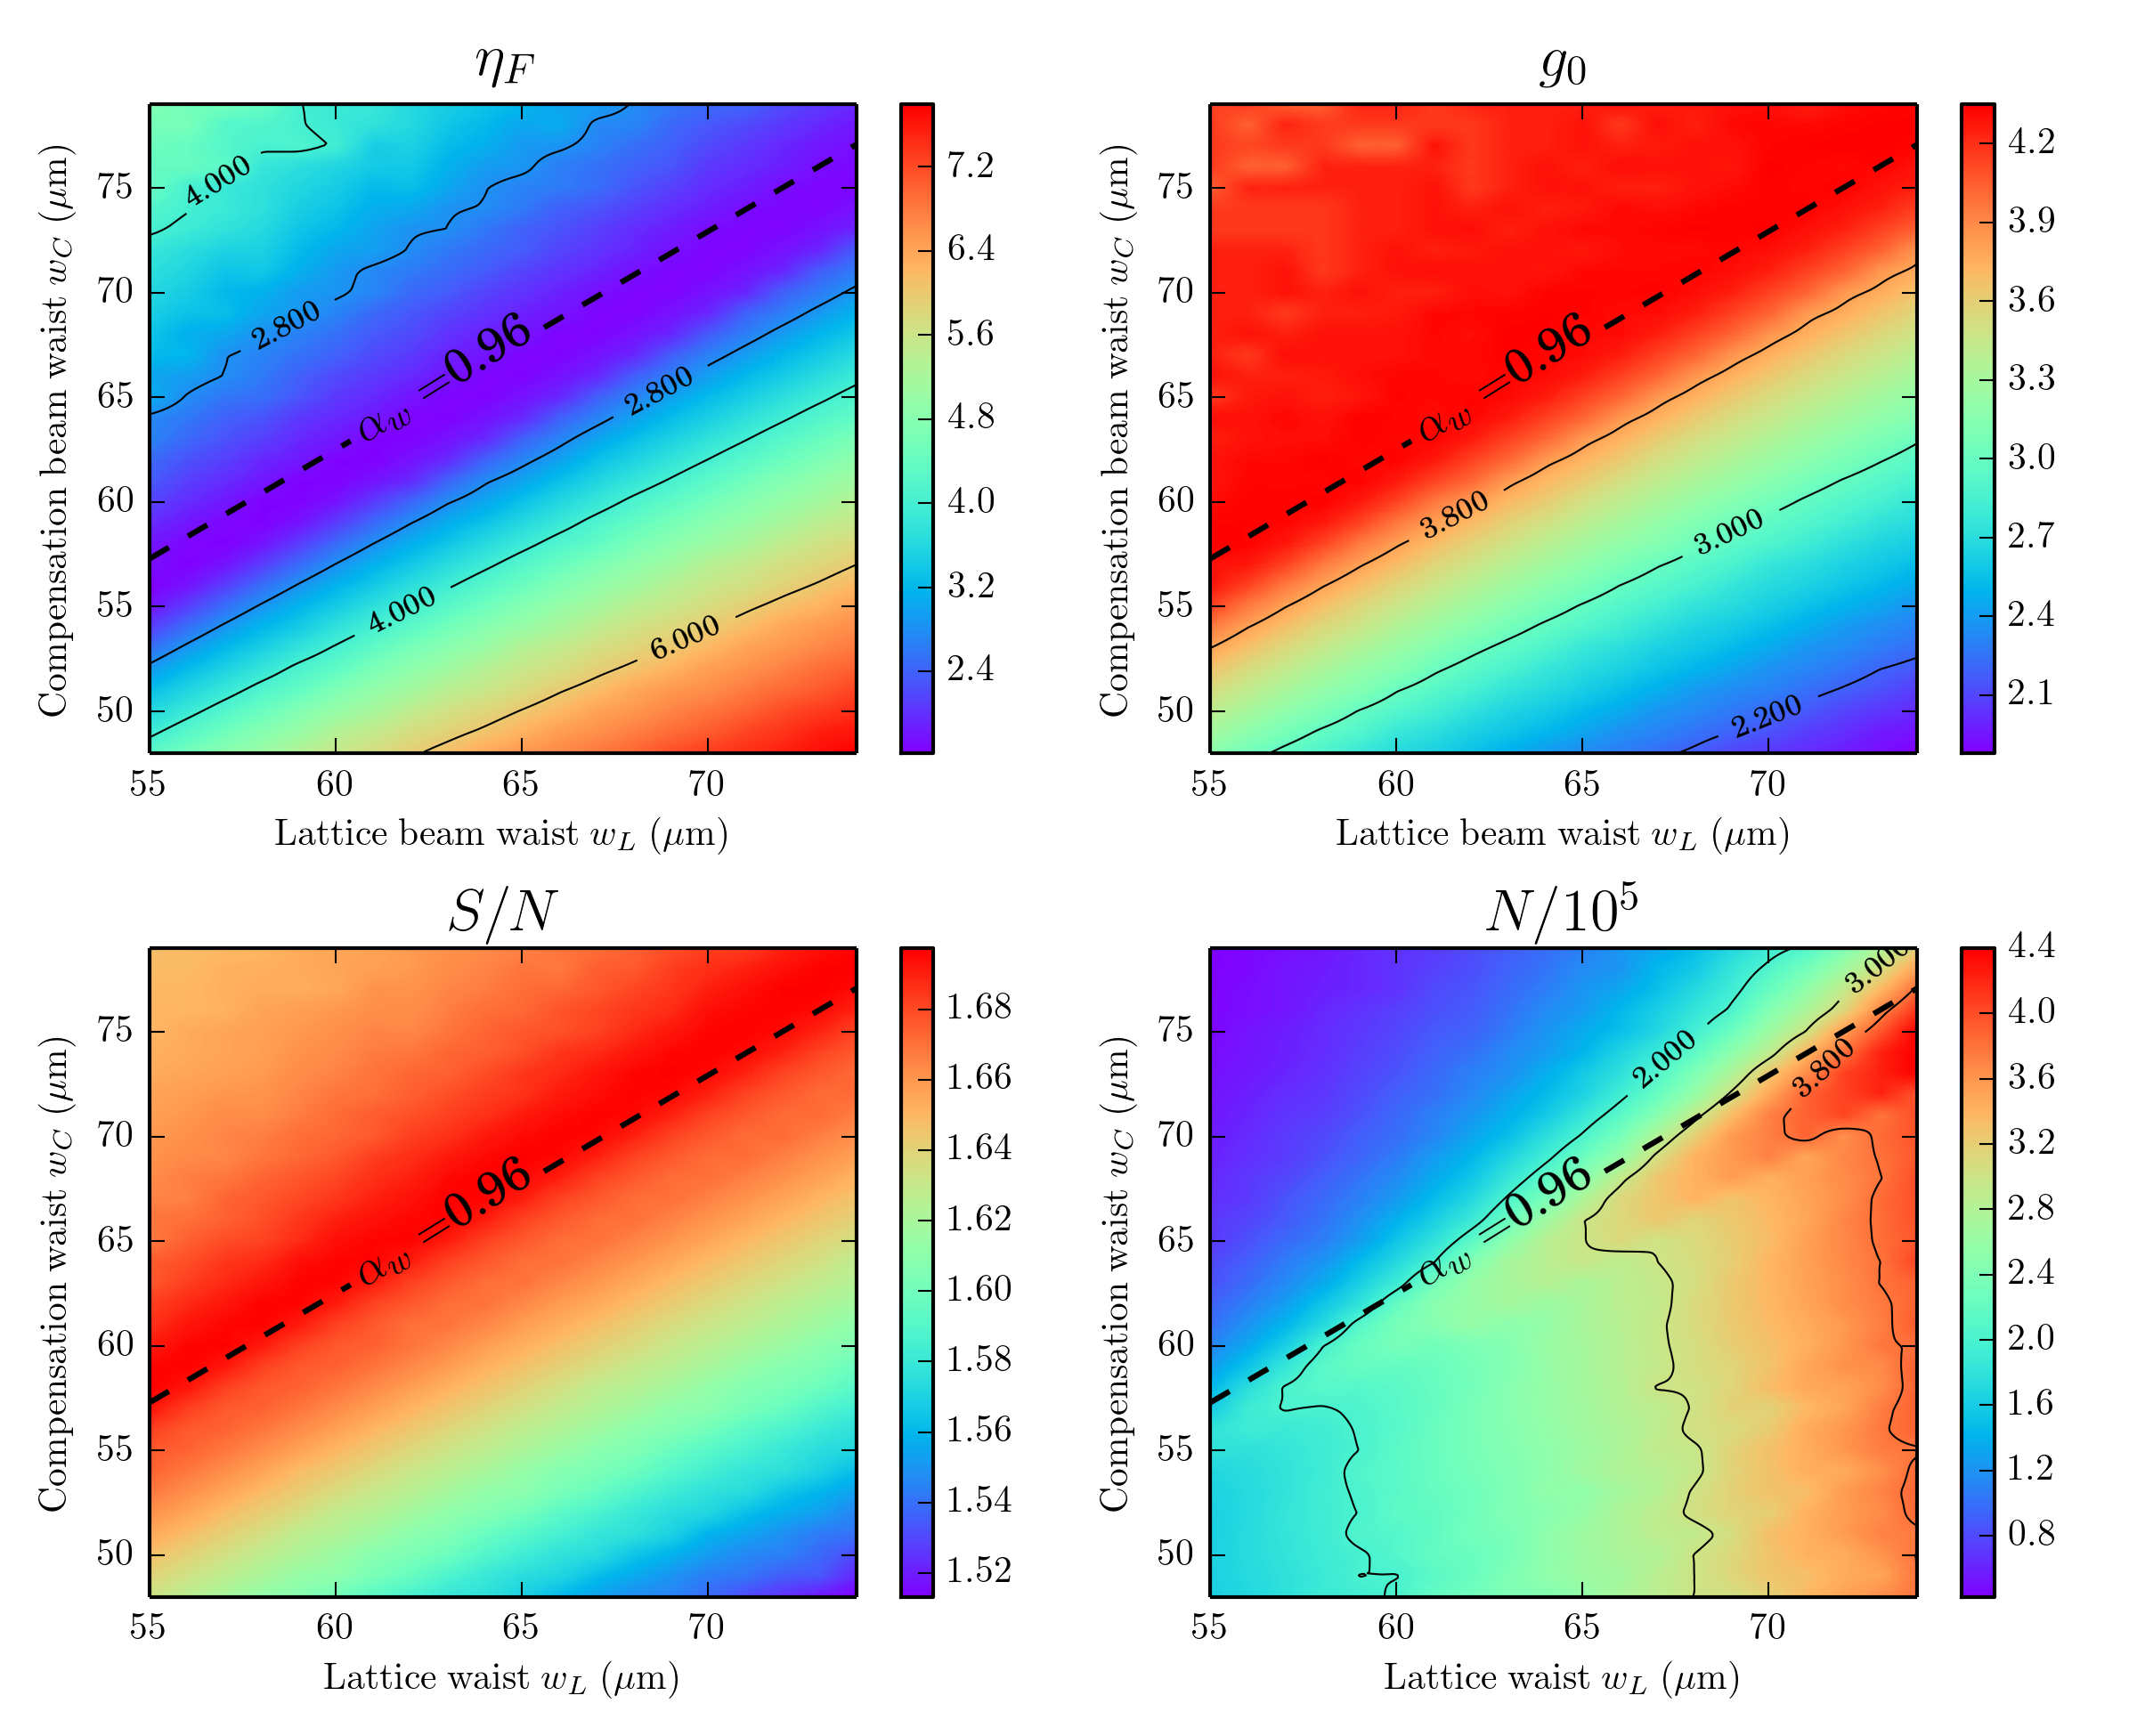
\includegraphics[width=0.65\textwidth]{figures_hubbard-lda/etaF-wIRwGR_r032.png}
\caption{LDA results. At each value of $w_{L}$, $w_{C}$ the compensation is
adjusted so that the radius of the sample is 0.32\,$w_{L}$. Calculation
performed at $T=0.12\,E_{R}$ which amounts to $T=3t$ at the center of the
7\,$E_{R}$ lattice.}
    \label{fig:optimize_lock}
\end{figure}

\paragraph{Observations.}
\begin{itemize}
\item With $\awaist\approx 0.96$ the best values of both $\eta_{F}$ and $S/N$
can be achived for a sample that has HWHM = 0.32\,$w_{L}$, and this is lockable
up to 30\,$E_{R}$.   Attaining this with $N=300,000$ atoms requires a lattice
beam waist $w_{L}=68\,\mu$m. 

\item  Reducing the compensation to satsify the locking requirements sets the
best  $\eta_{F}$ and $S/N$ at $\eta_{F} \approx 1.8$ and $S/N\approx 1.7$ (for
$T=3t$ at the center).   

\item  $\eta_{F}$ and $S/N$ can be optimized independently at $\awaist = 1.06$
and $\awaist = 0.96$ respectively as was shown in the previosu section.   When
setting the radius at 0.32\,$w_{L}$ both $\eta_{F}$ and $S/N$ are optimized
almost simultaneously for $\awaist \approx 0.96$. 

\end{itemize}

\subsection{ Resulting profiles }

Below we plot the resulting LDA profiles to further illustrate some of the
results obtained above and motivate our conclusions for the future improvements
of the setup.  
 

\begin{itemize} 

\item We start out by showing our current setup,  $w_{L}=47\,\mu$,
$w_{C}=40\,\mu$m with the optimal compensation obtained at $T=0.4\,E_{R}$
($T=10.1t$) and $T=0.2\,E_{R}$ ($T=5.1t$) in Figs.~\ref{fig:profiles000} and
\ref{fig:profiles001} respectively.    With our current setup and optimal
compensation we cannot run the LDA at temperatures below $T=5.1t$.  The sample
extends so much into the lattice beams that the local $T/t$ at the edge goes
down to $T/t=1.5$ which is right at the limit of validity of the HTSE. 
\begin{figure}[H]
        \centering
        \begin{subfigure}[t]{0.42\textwidth}
		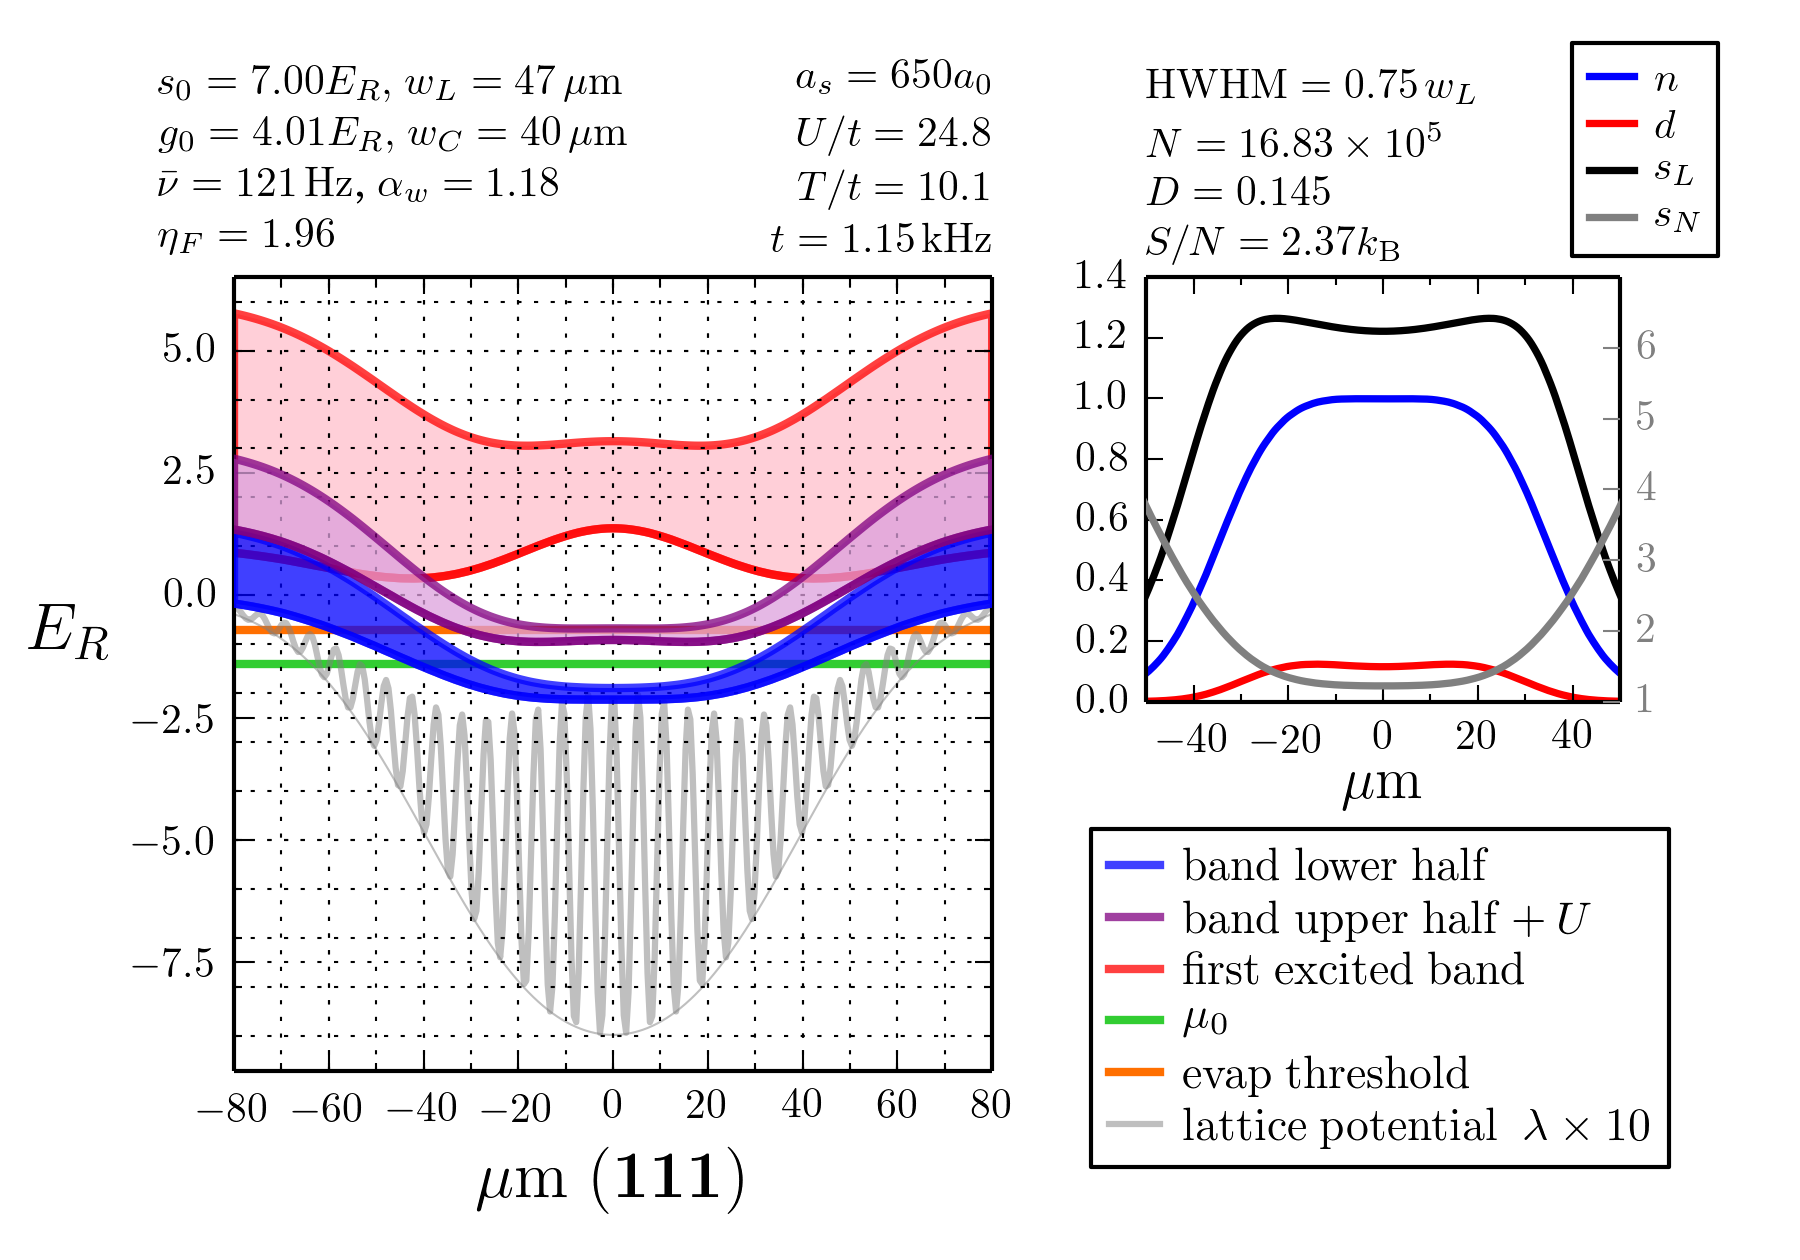
\includegraphics[width=\textwidth]{figures_hubbard-lda/000.png}
\caption{ }
                \label{fig:profiles000}
        \end{subfigure}%
        ~~ %add desired spacing between images, e. g. ~, \quad, \qquad etc.
          %(or a blank line to force the subfigure onto a new line)
        \begin{subfigure}[t]{0.42\textwidth}
		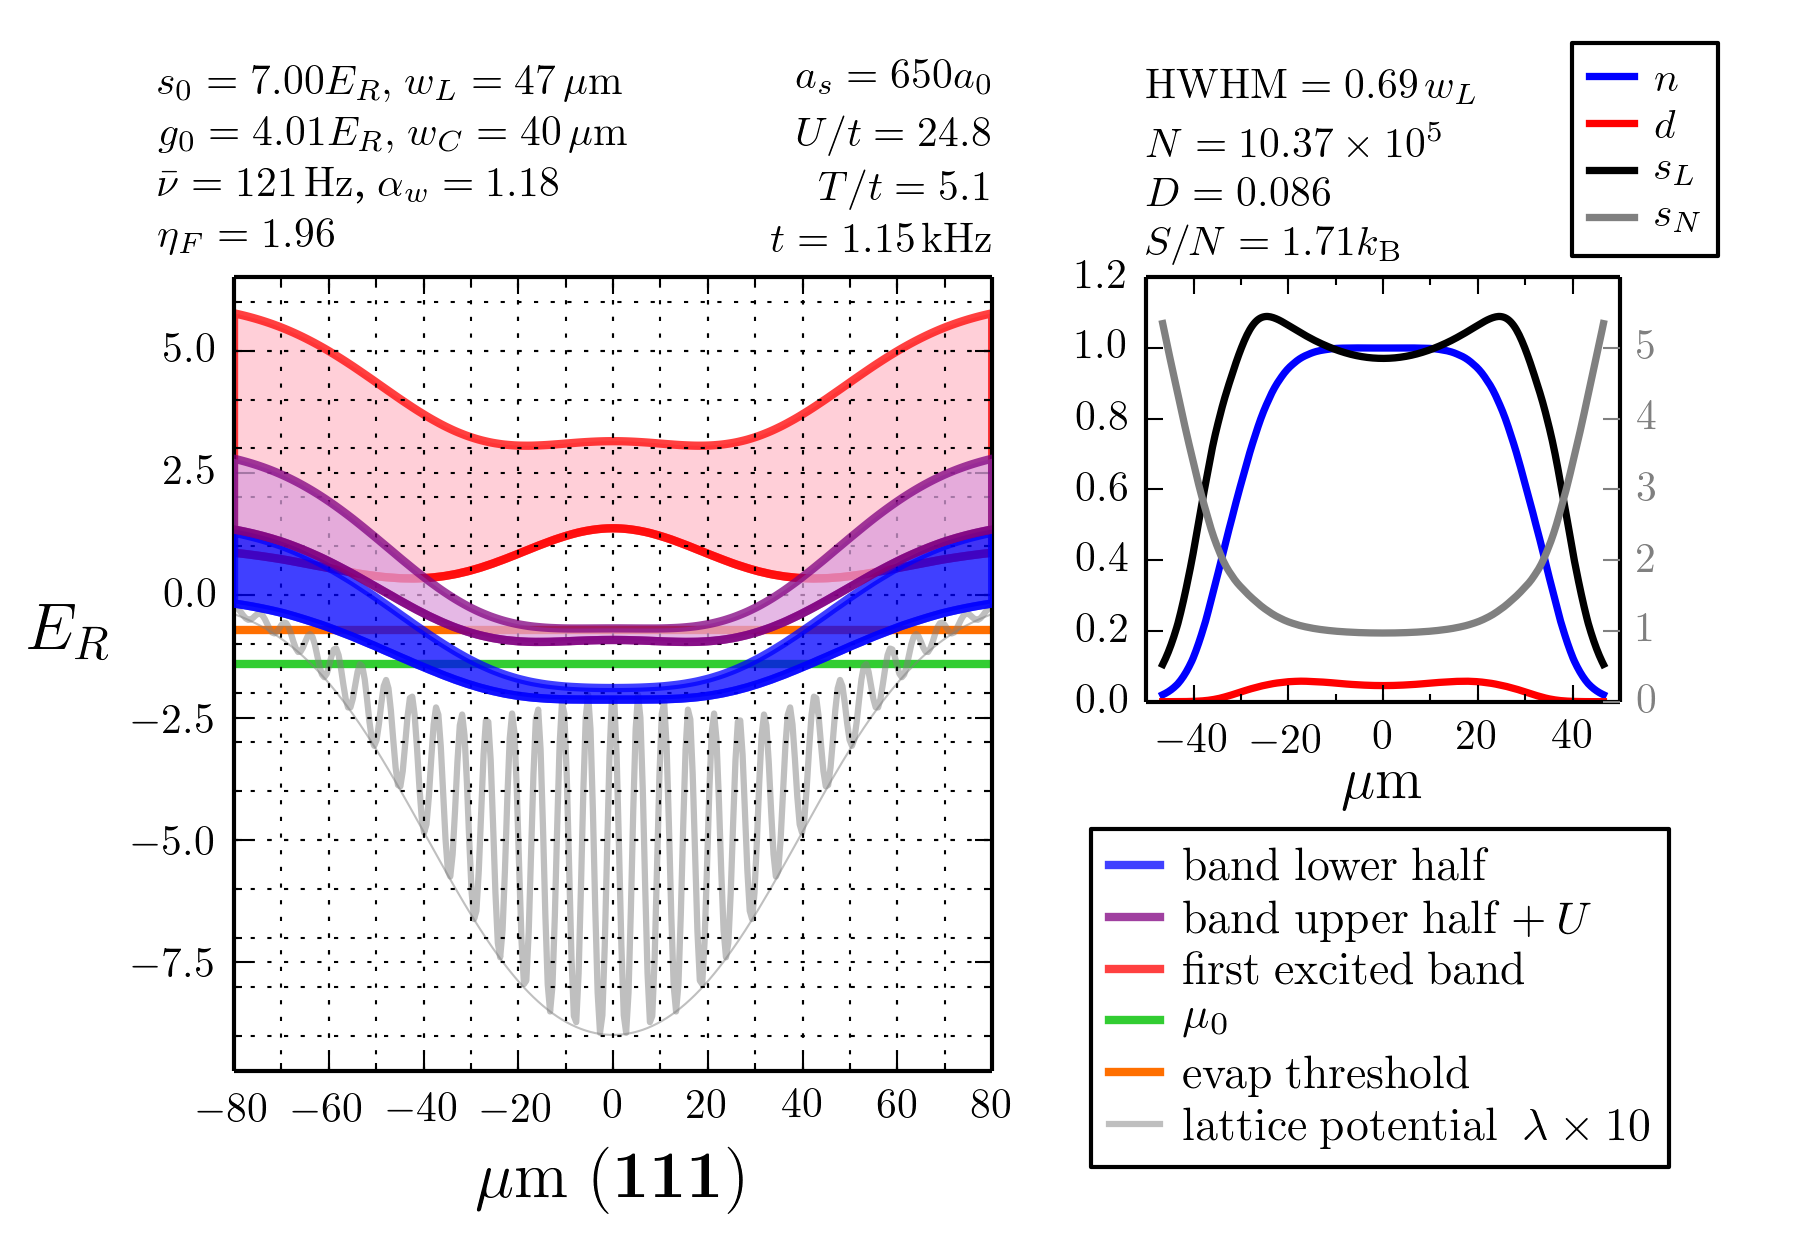
\includegraphics[width=\textwidth]{figures_hubbard-lda/001.png}
\caption{ }
                \label{fig:profiles001}
        \end{subfigure}
	\caption{}
%\label{fig:}
\end{figure}

\item  In our current Bragg spectroscopy experiments we use $N=200,000$ atoms,
so for our beam waists we have to reduce the compensation in order to achieve a
density of one atom per site at the center.    The LDA result for our current
atom number and potential is shown for $T=0.2\,E_{R}$ ($T/t=5.1$) and
$T=0.12\,E_{R}$ ($T/t=3$) in Figs.~\ref{fig:profiles002} and
\ref{fig:profiles003} respectively. SAY SOMETHING HERE ABOUT ETAF FOR THIS SETUP
ALSO COMPARED TO ETAF IN THE SETUP WITH OPTIMAL COMPENSATION.
\begin{figure}[H]
        \centering
        \begin{subfigure}[t]{0.42\textwidth}
		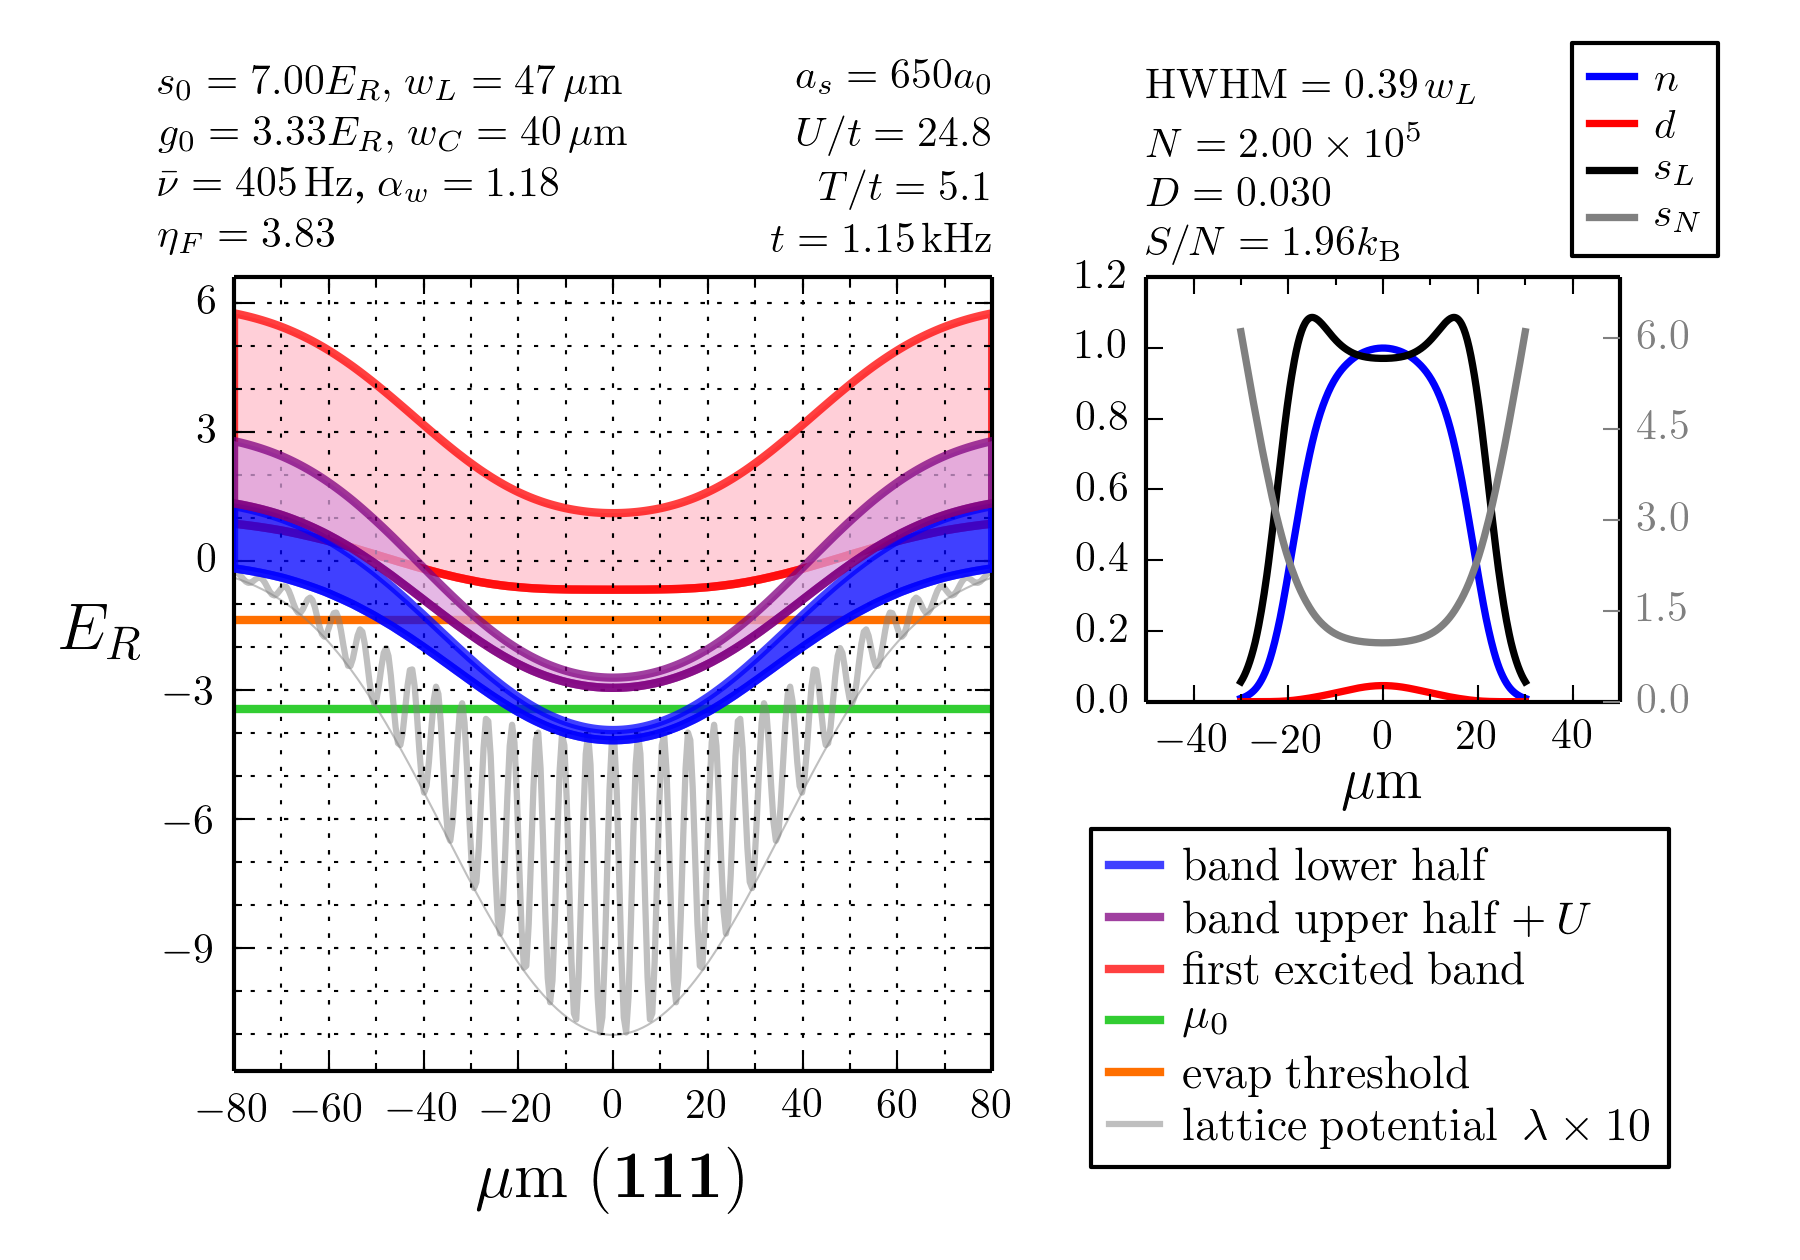
\includegraphics[width=\textwidth]{figures_hubbard-lda/002.png}
\caption{ }
                \label{fig:profiles002}
        \end{subfigure}%
        ~~ %add desired spacing between images, e. g. ~, \quad, \qquad etc.
          %(or a blank line to force the subfigure onto a new line)
        \begin{subfigure}[t]{0.42\textwidth}
		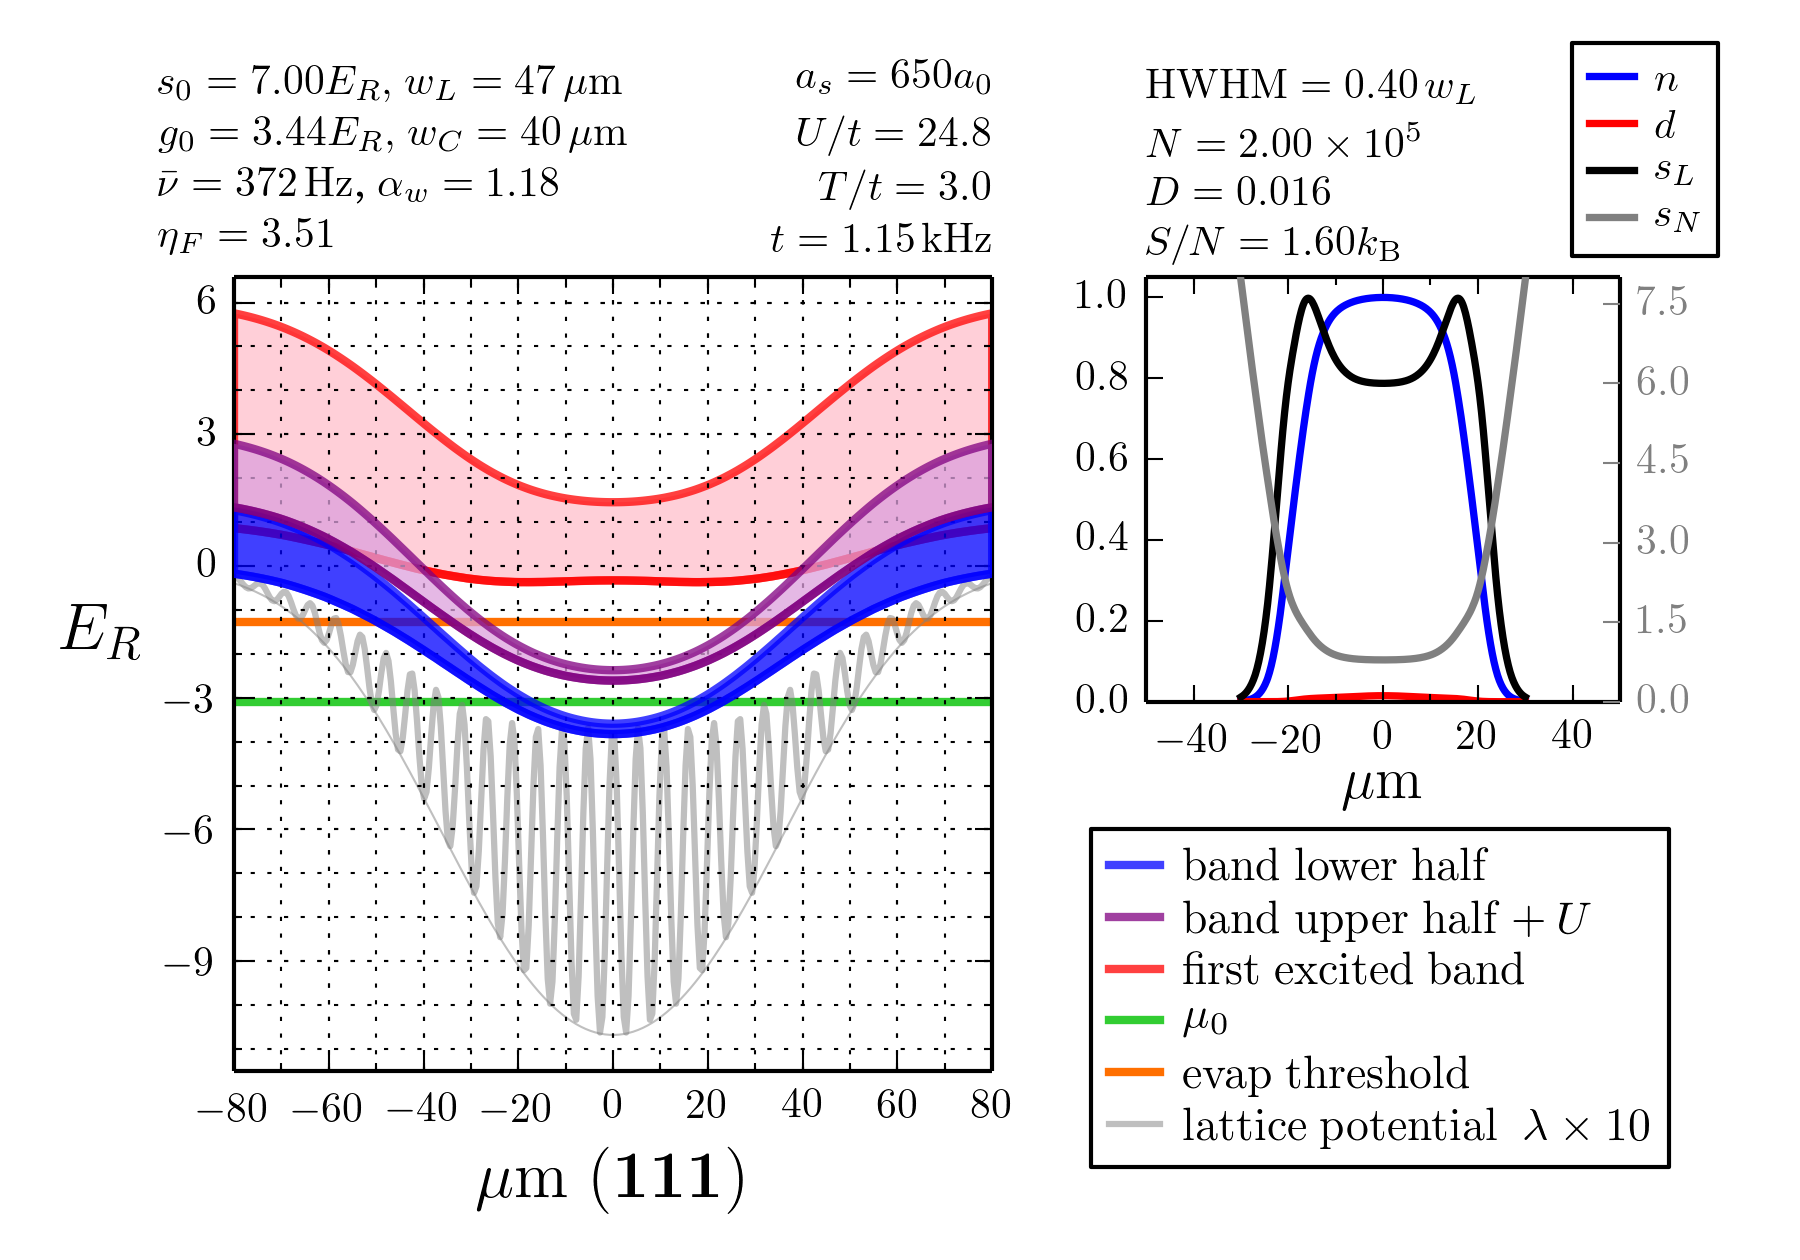
\includegraphics[width=\textwidth]{figures_hubbard-lda/003.png}
\caption{ }
                \label{fig:profiles003}
        \end{subfigure}
	\caption{}
%\label{fig:}
\end{figure}

\item In Fig.~\ref{fig:profiles005} we show the result for a uniform lattice
and harmonic confinement,  setting $N=200,000$ and $n=1$ at the center at a
temperature $T=0.12\,E_{R}$.    By comparing $\eta_{F}$ and $S/N$ to our
current setup we can see that in the uniform lattice the situation for
evporation is much less favorable ($\eta_{F} \approx 20$) but as far as entropy
redistribution the situations are very similar ($S/N\approx 1.6k_{\text{B}}$
for 200,00 atoms. 
\begin{figure}[H]
        \centering
		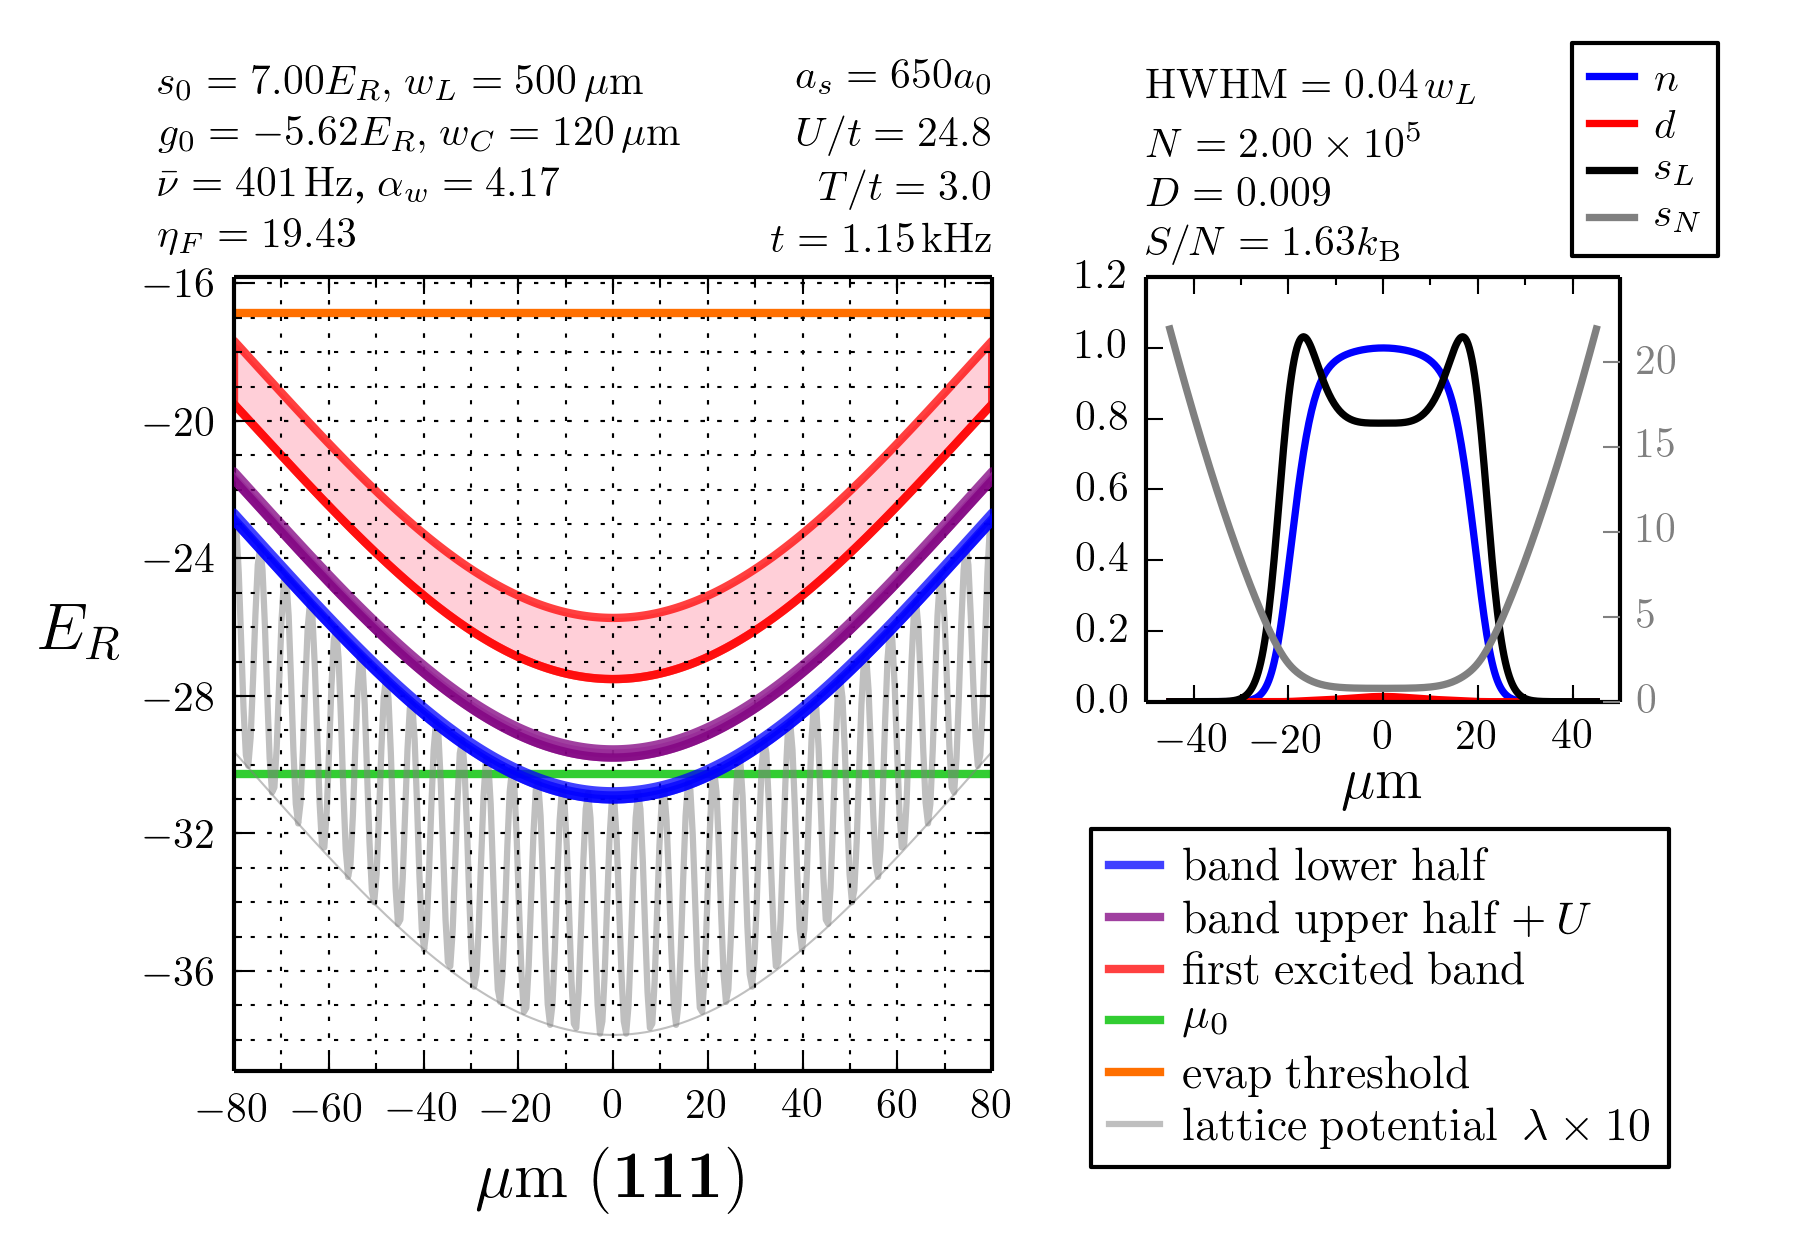
\includegraphics[width=0.42\textwidth]{figures_hubbard-lda/005.png}
	\caption{}
                \label{fig:profiles005}
%\label{fig:}
\end{figure}

\item Next we show the proposed scenario for our future implementation.  We use
a lattice beam waist $w_{L}=68\,\mu$m.  With compensation beam waists in the
range 68\,$\mu$m $< w_{C} < $ 75\,$\mu$m,  that is around $\awaist = 0.96$, we
can make samples that have good $\eta_{F}$ and $S/N$ characteristics.
Additianly for these values of $\awaist$ the resulting sample occupies a small
fraction of the beam waist such that the lattice can be locked to a depth of up
to $\approx 30\,E_{R}$.    The choice of $w_{L}$ sets the scale for the atom
number, which can be between 200,000 and 450,000 atoms in this range.   Results
are shown in Figs.~\ref{fig:profiles006} to ~\ref{fig:profiles008}.  
\begin{figure}[H]
        \centering
        \begin{subfigure}[t]{0.42\textwidth}
		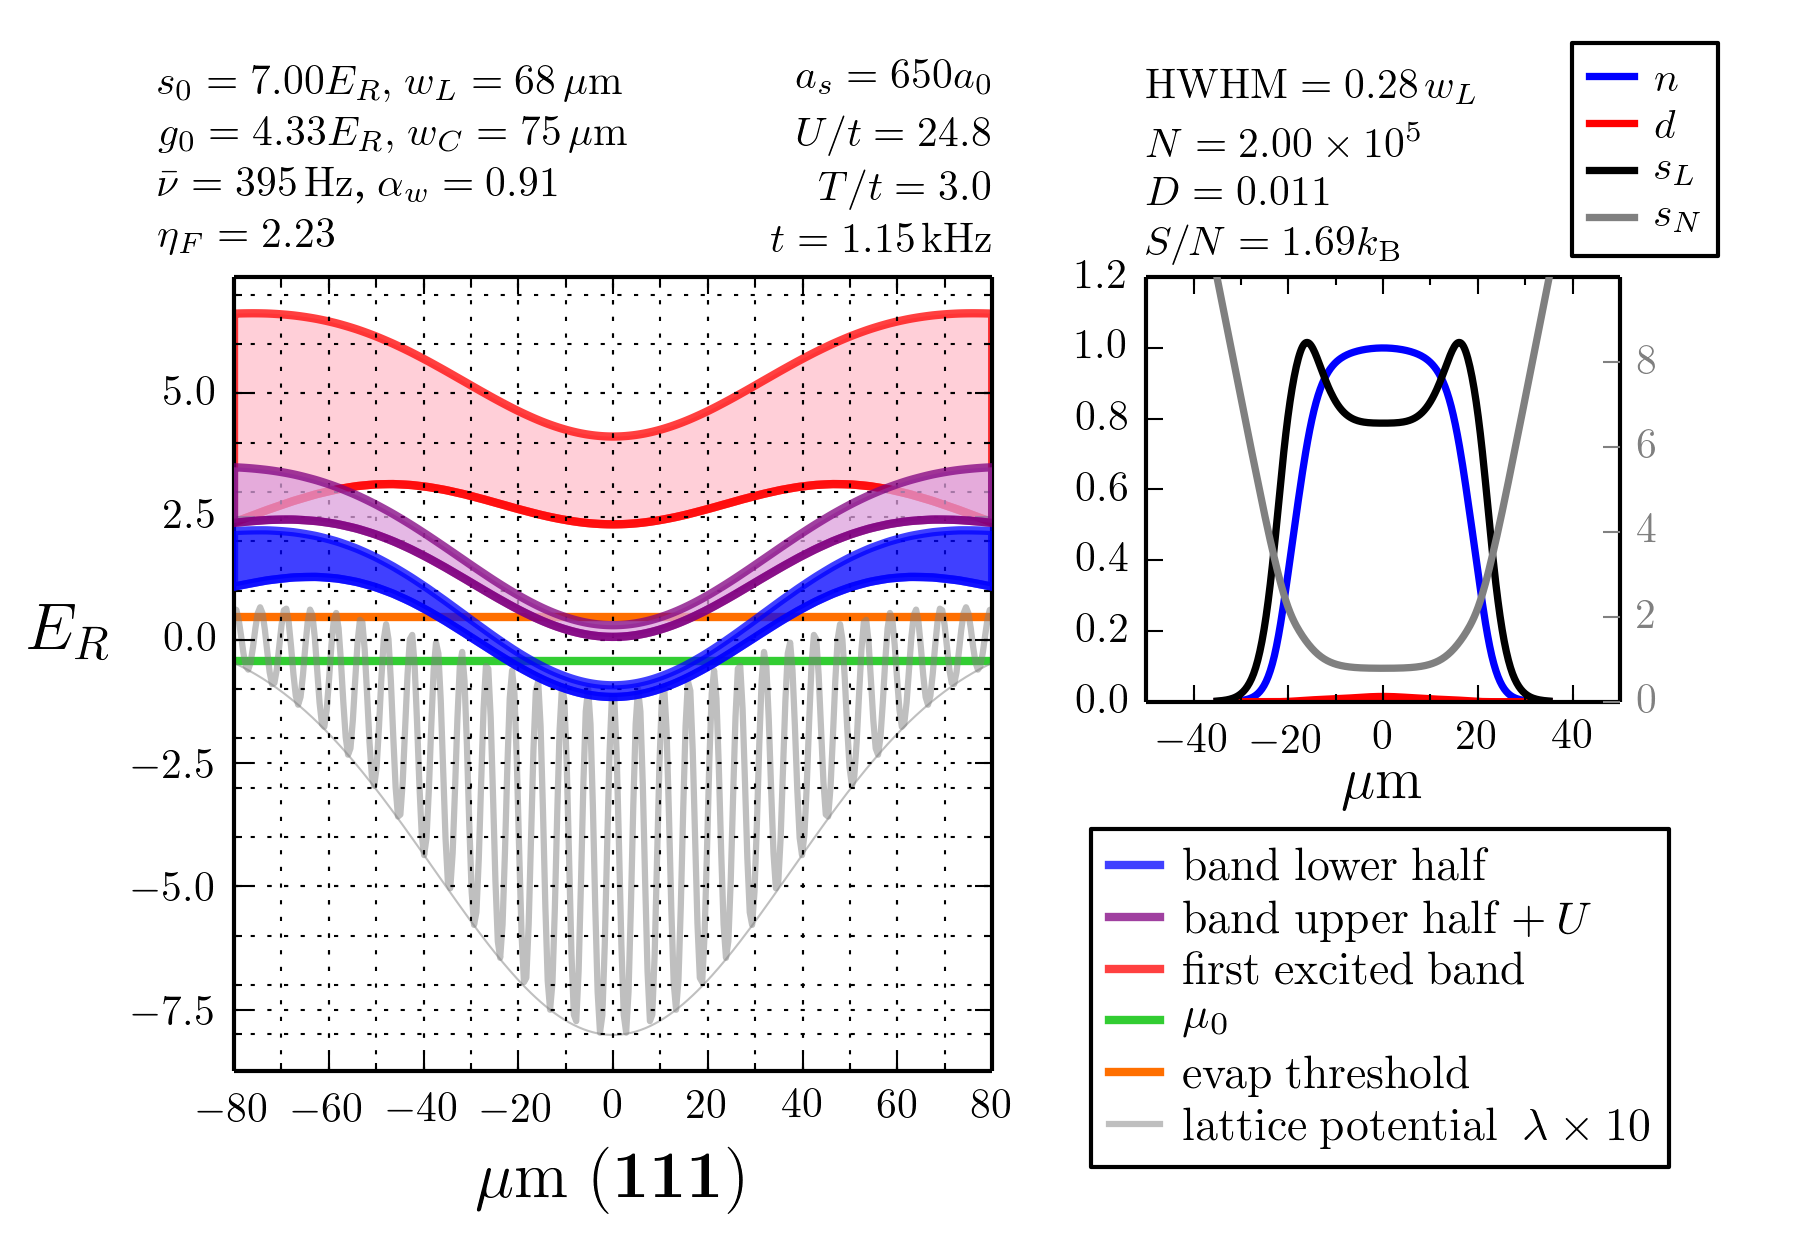
\includegraphics[width=\textwidth]{figures_hubbard-lda/006.png}
\caption{ }
                \label{fig:profiles006}
        \end{subfigure}%
        ~~ %add desired spacing between images, e. g. ~, \quad, \qquad etc.
          %(or a blank line to force the subfigure onto a new line)
        \begin{subfigure}[t]{0.42\textwidth}
		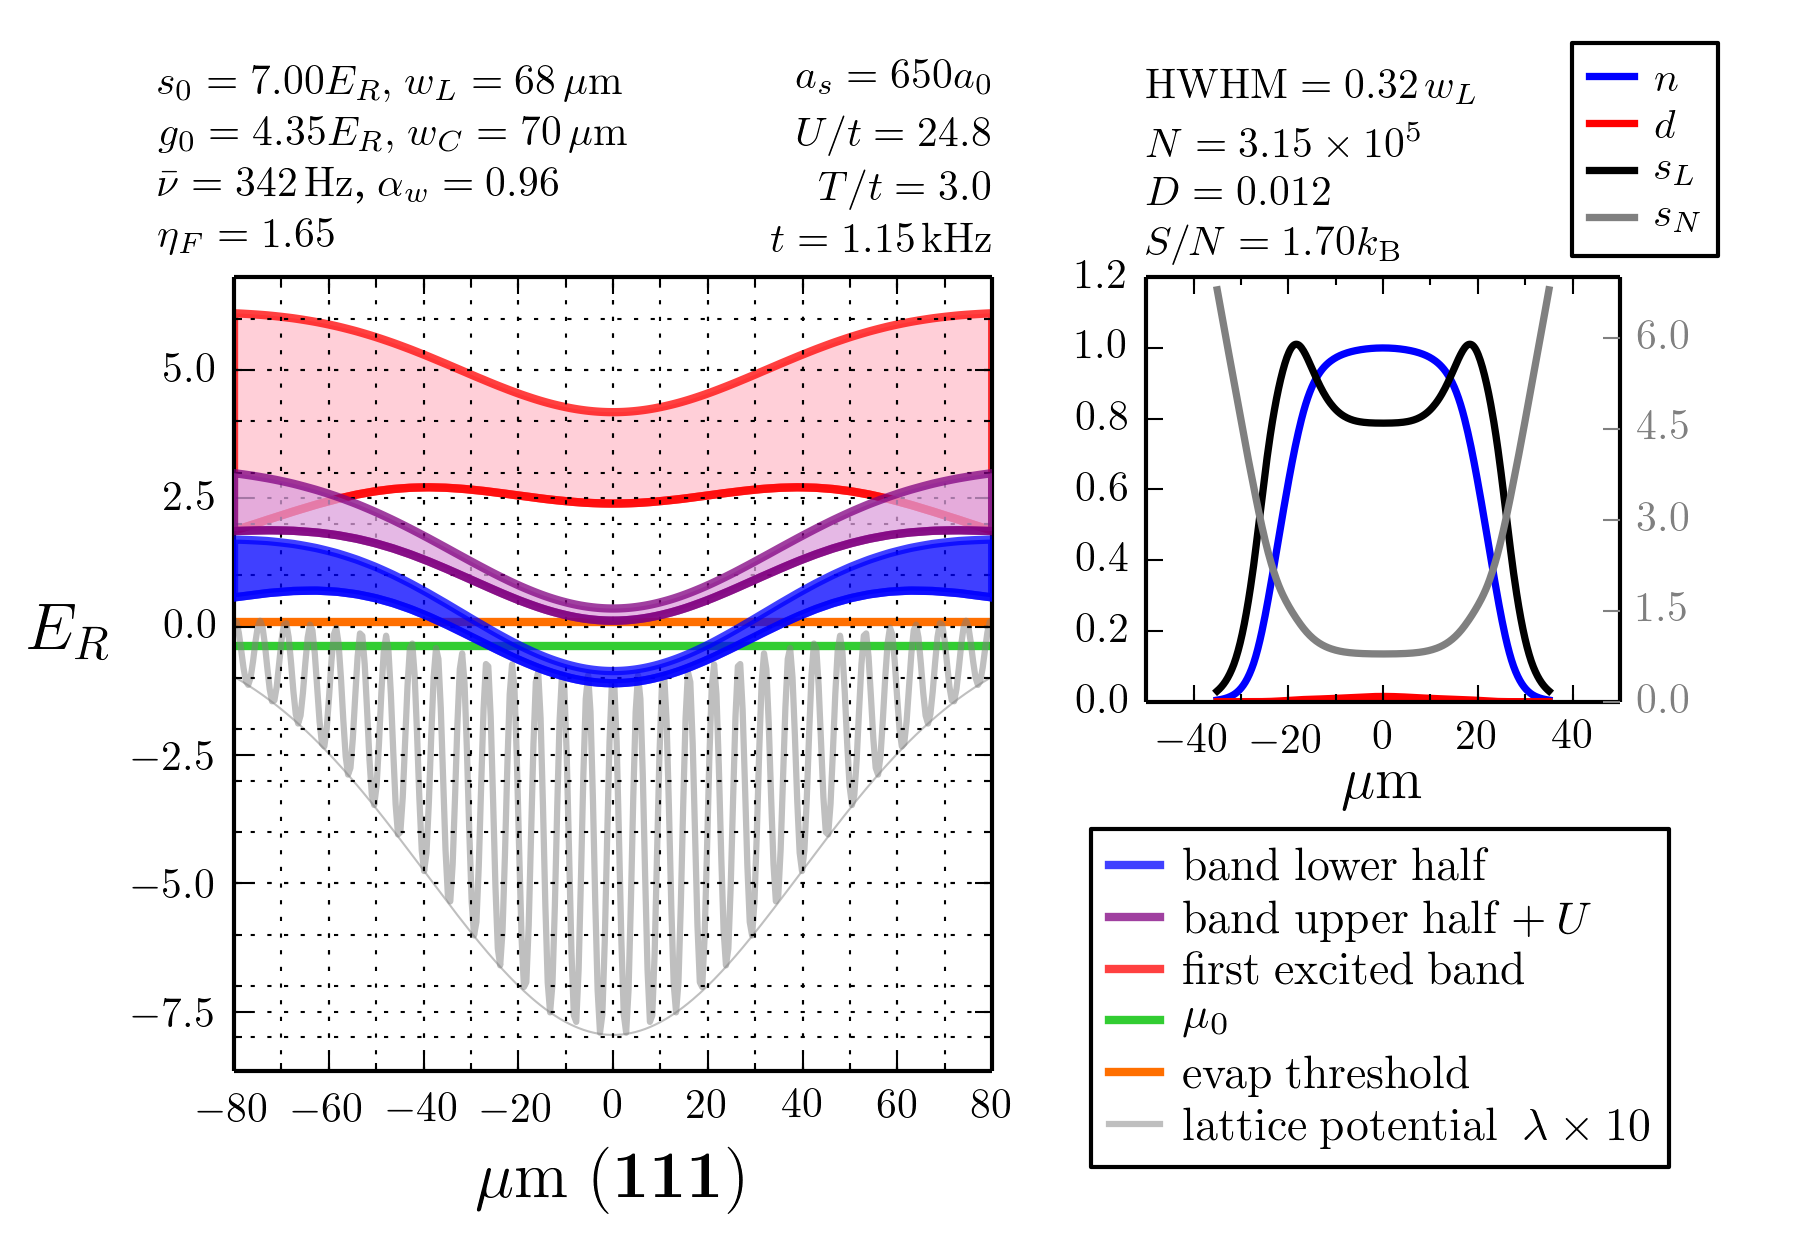
\includegraphics[width=\textwidth]{figures_hubbard-lda/007.png}
\caption{ }
                \label{fig:profiles007}
        \end{subfigure}

        \begin{subfigure}[t]{0.42\textwidth}
		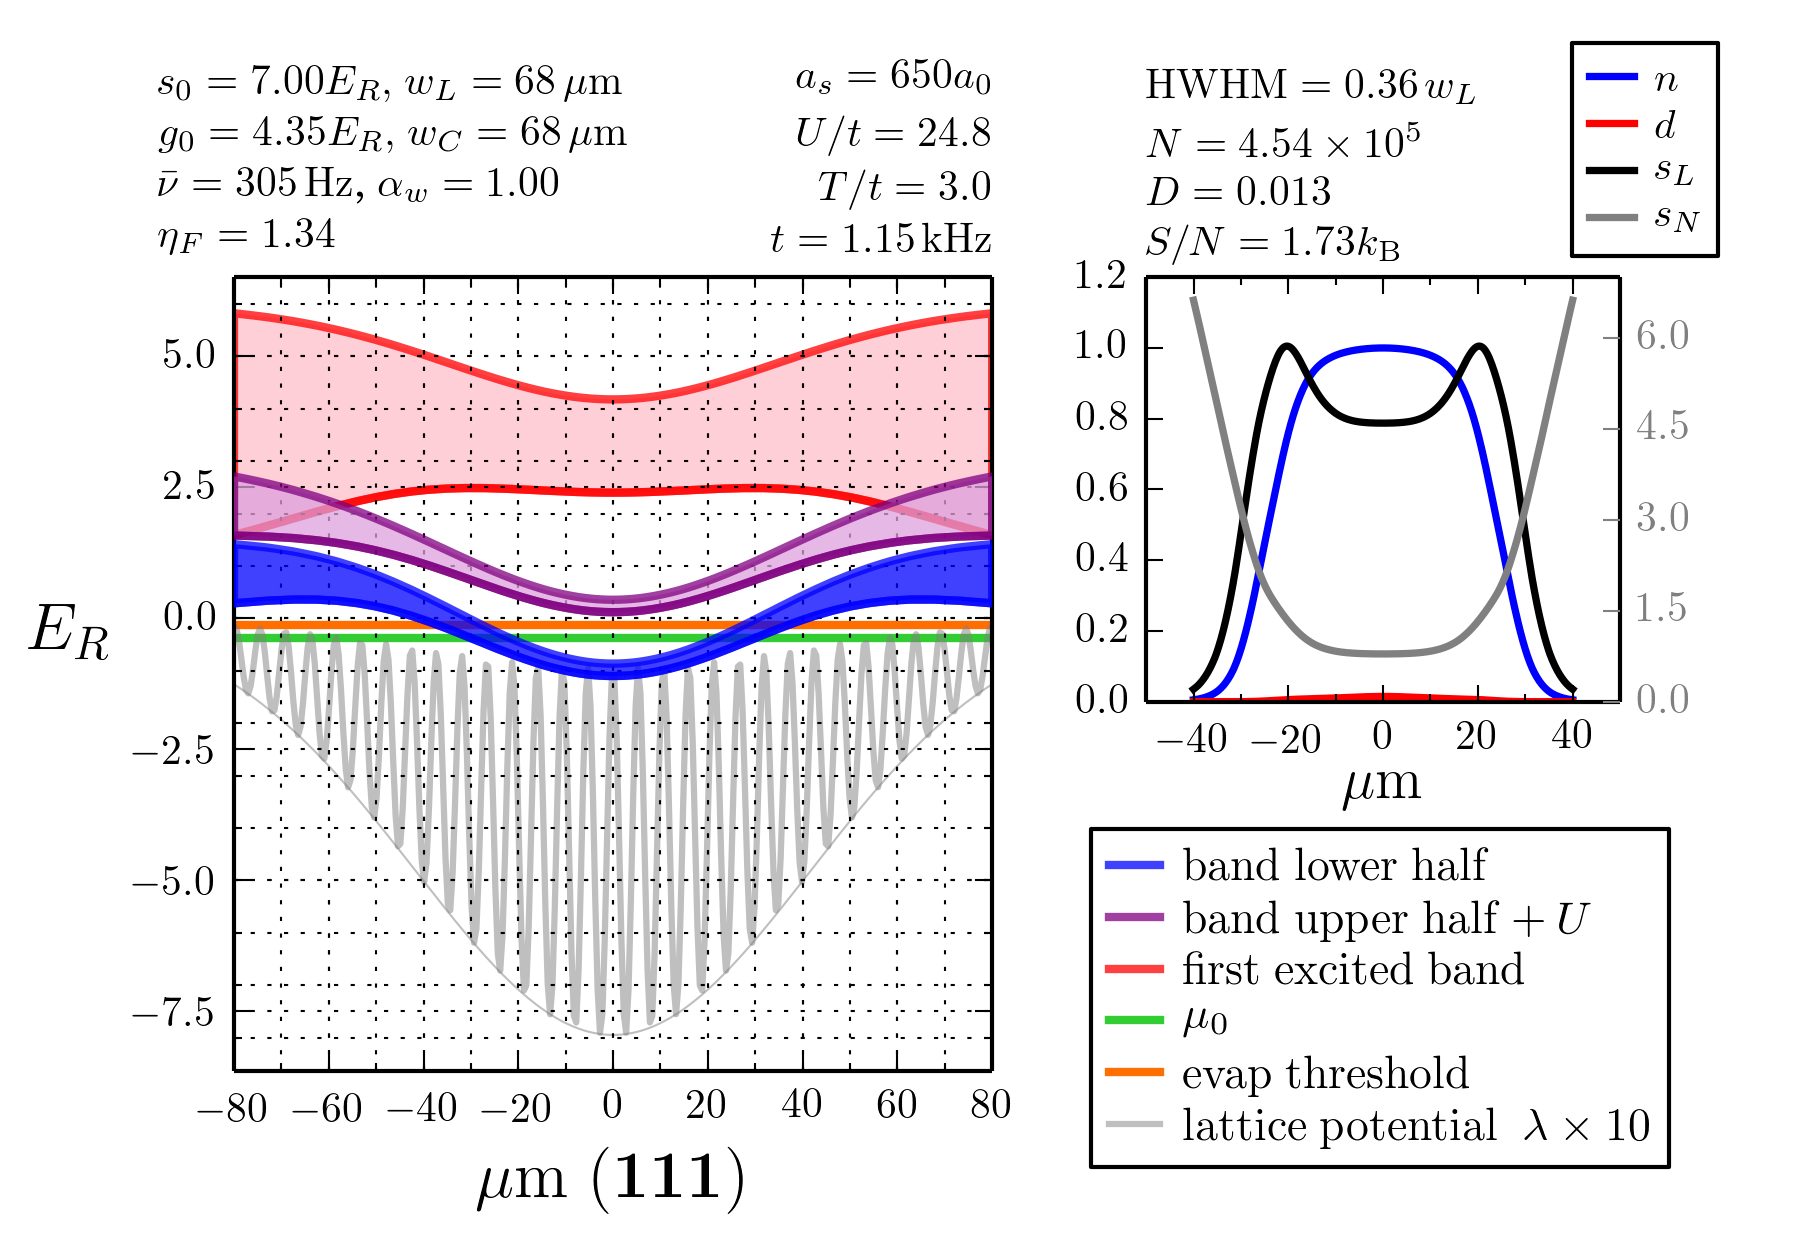
\includegraphics[width=\textwidth]{figures_hubbard-lda/008.png}
\caption{ }
                \label{fig:profiles008}
        \end{subfigure}
	\caption{}
%\label{fig:}
\end{figure}

\end{itemize}

\newpage

The profiles that are shown in Fig.~\ref{fig:HTSE_full-band-profiles} are
calculated at a temperature $T=1.8t$, which is near the lowest temperature
value accessible with the HTSE.   The chemical potential, measured from the
lowest energy level available to the system (the bottom of the band) is set to
$\mu=6t +U/2$ to guarantee half-filling at the center.  \footnote{ The $6t$
here is half the bandwidth.  Note that in typical treatments the chemical
potential is always measured from the center of the lowest band, so the $6t$
will be omitted. In that case the chemical potential associated with
half-filling Will be $U/2$.  Some treatments even shift the zero of energy by
$U/2$ so that half filling occurs nominally at $\mu$=0 regardless of $U$. } We
used a value of $U=24.9t$,  given by the scattering length, which is set at
650$a_{0}$.   

Plugging in these values we obtain $\mu\approx 18 t$  or $T/\mu \approx 1.8/18
= 0.1 $.  When the temperature is so low, one can safely assume that $\mu
\approx E_{F}$,  so this system would have  $T/T_{F}=0.06$ at an overall
entropy per particle of $S/N=1.94\kb$.  If the sample was obtained by ramping
up the lattice adiabatically starting from a harmonic trap, then the initial
entropy in the harmonic trap should also be 1.94\kb.  In the harmonic trap this
corresponds to $T/T_{F} = S/(\pi^{2} N) \approx 0.2$.  

We conclude from these rough estimates that as the sample gets loaded into the
lattice it gets adiabatically cooled, its value of $T/T_{F}$ is reduced.  This
is in contrast with the result obtained in~\cite{Kohl2006} where it was
concluded that loading a gas adiabatically from a harmonic trap to a deep
optical lattice would adiabatically heat the gas.   In this case we are
considering interactions and not neglecting the width of the lowest band.  Our
observation that the gas is adiabatically cooled as it is loaded into the
lattice are consistent with the results from~\cite{Paiva2011}.   

(NOTE: I NEED TO ASK THEREZA ABOUT THESE REMARKS TO CHECK THAT I AM NOT MAKING
A MISTAKE. 

The main question is whether it is ok to take $\mu=E_{F}$ since $\mu$ is in
the Mott gap.   Should one take  $E_{F}=12t$ in that case, since the top of the
band is the largest energy state that could potentially be occupied?? )


\subsubsection{ Enlarging the Mott state}  

In this section we consider our experimental setup
($w_{\text{L}}=47\,\mu\mathrm{m}$, $w_{\text{C}}=40\,\mu\mathrm{m}$)  and we
vary the amount of compensation.   What we find is that if no compensation is
used, then the number of atoms has to be very small in order to achieve
half-filling at the center.     On the other hand,  when using compensation one
can still hold a large number of atoms and maintain half-filling.   This leads
to the concept of enlarging the Mott state ( or N\'{e}el state if your
temperature is low enough)  which can be a very dramatic effect as was shown in
the paper by Mathy, Huse and Hulet~\cite{Mathy2012}.  

The effect of enlarging the Mott state is shown in
Fig.~\ref{fig:HTSE_enlarge-mott}, where we show the relationship between atom
number and compensation when the filling is set to $n=1$ at the center of the
cloud. This figure also shows the profile plots for no compensation and a
compensation of 3.05\,$E_{R}$,  in order to illustrate how the Mott plateau in
the density profile is enlarged for larger compensation.  
\begin{figure}
        \centering
        \begin{subfigure}[t]{0.32\textwidth}
		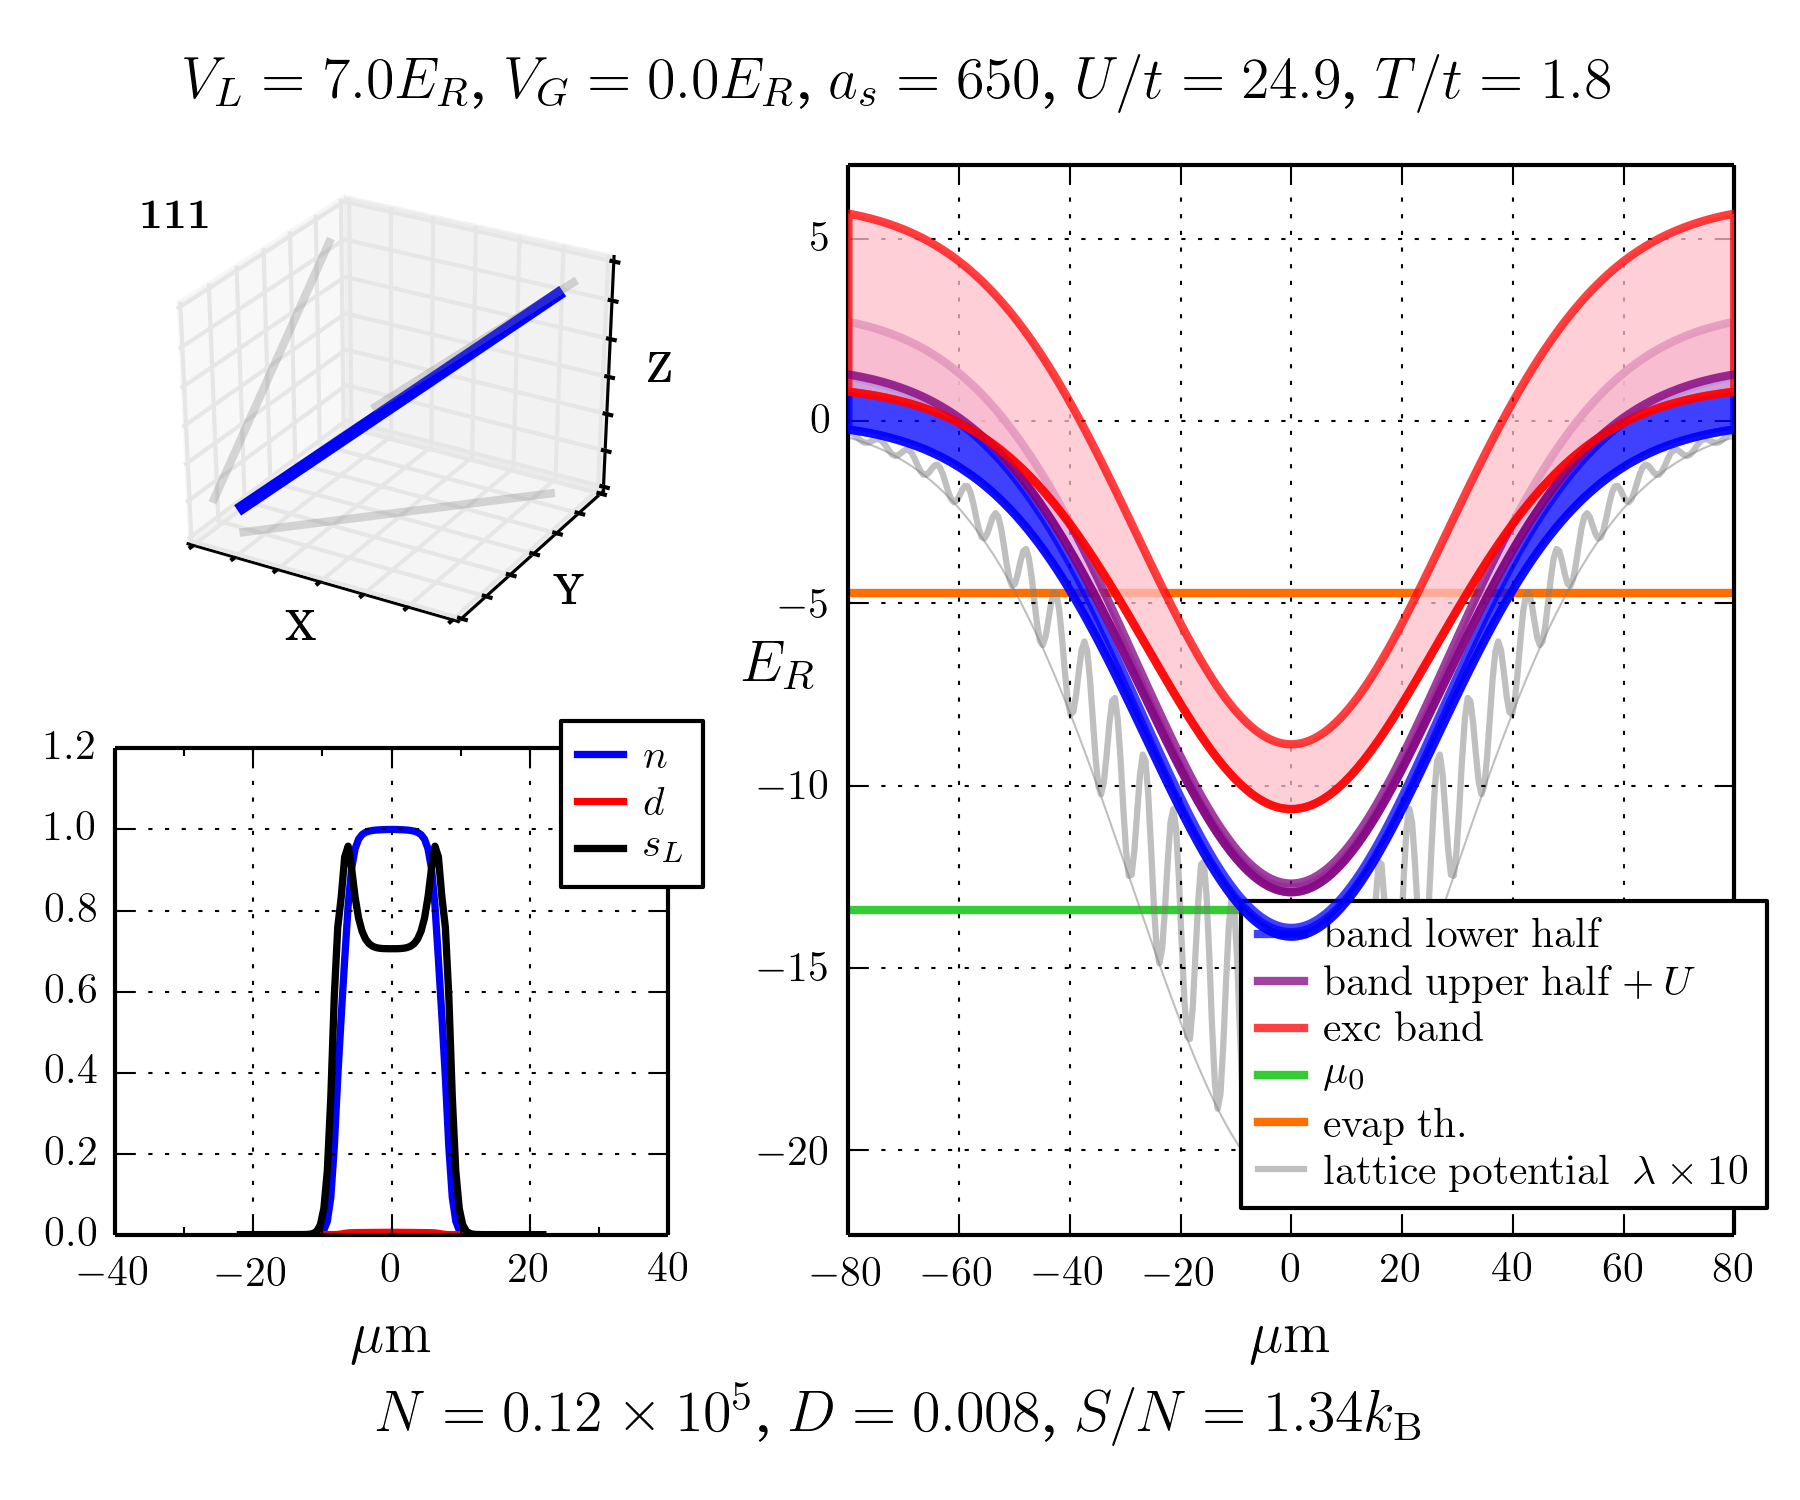
\includegraphics[width=\textwidth]{figures/ir47-gr40_7Er-comp0p0.png}
\caption{$w_{L}=47\,\mu$m and $w_{C}=40\,\mu$m without compensation.  }
                \label{fig:HTSE_enlarge-mott_a}
        \end{subfigure}%
        ~ %add desired spacing between images, e. g. ~, \quad, \qquad etc.
          %(or a blank line to force the subfigure onto a new line)
        \begin{subfigure}[t]{0.32\textwidth}
                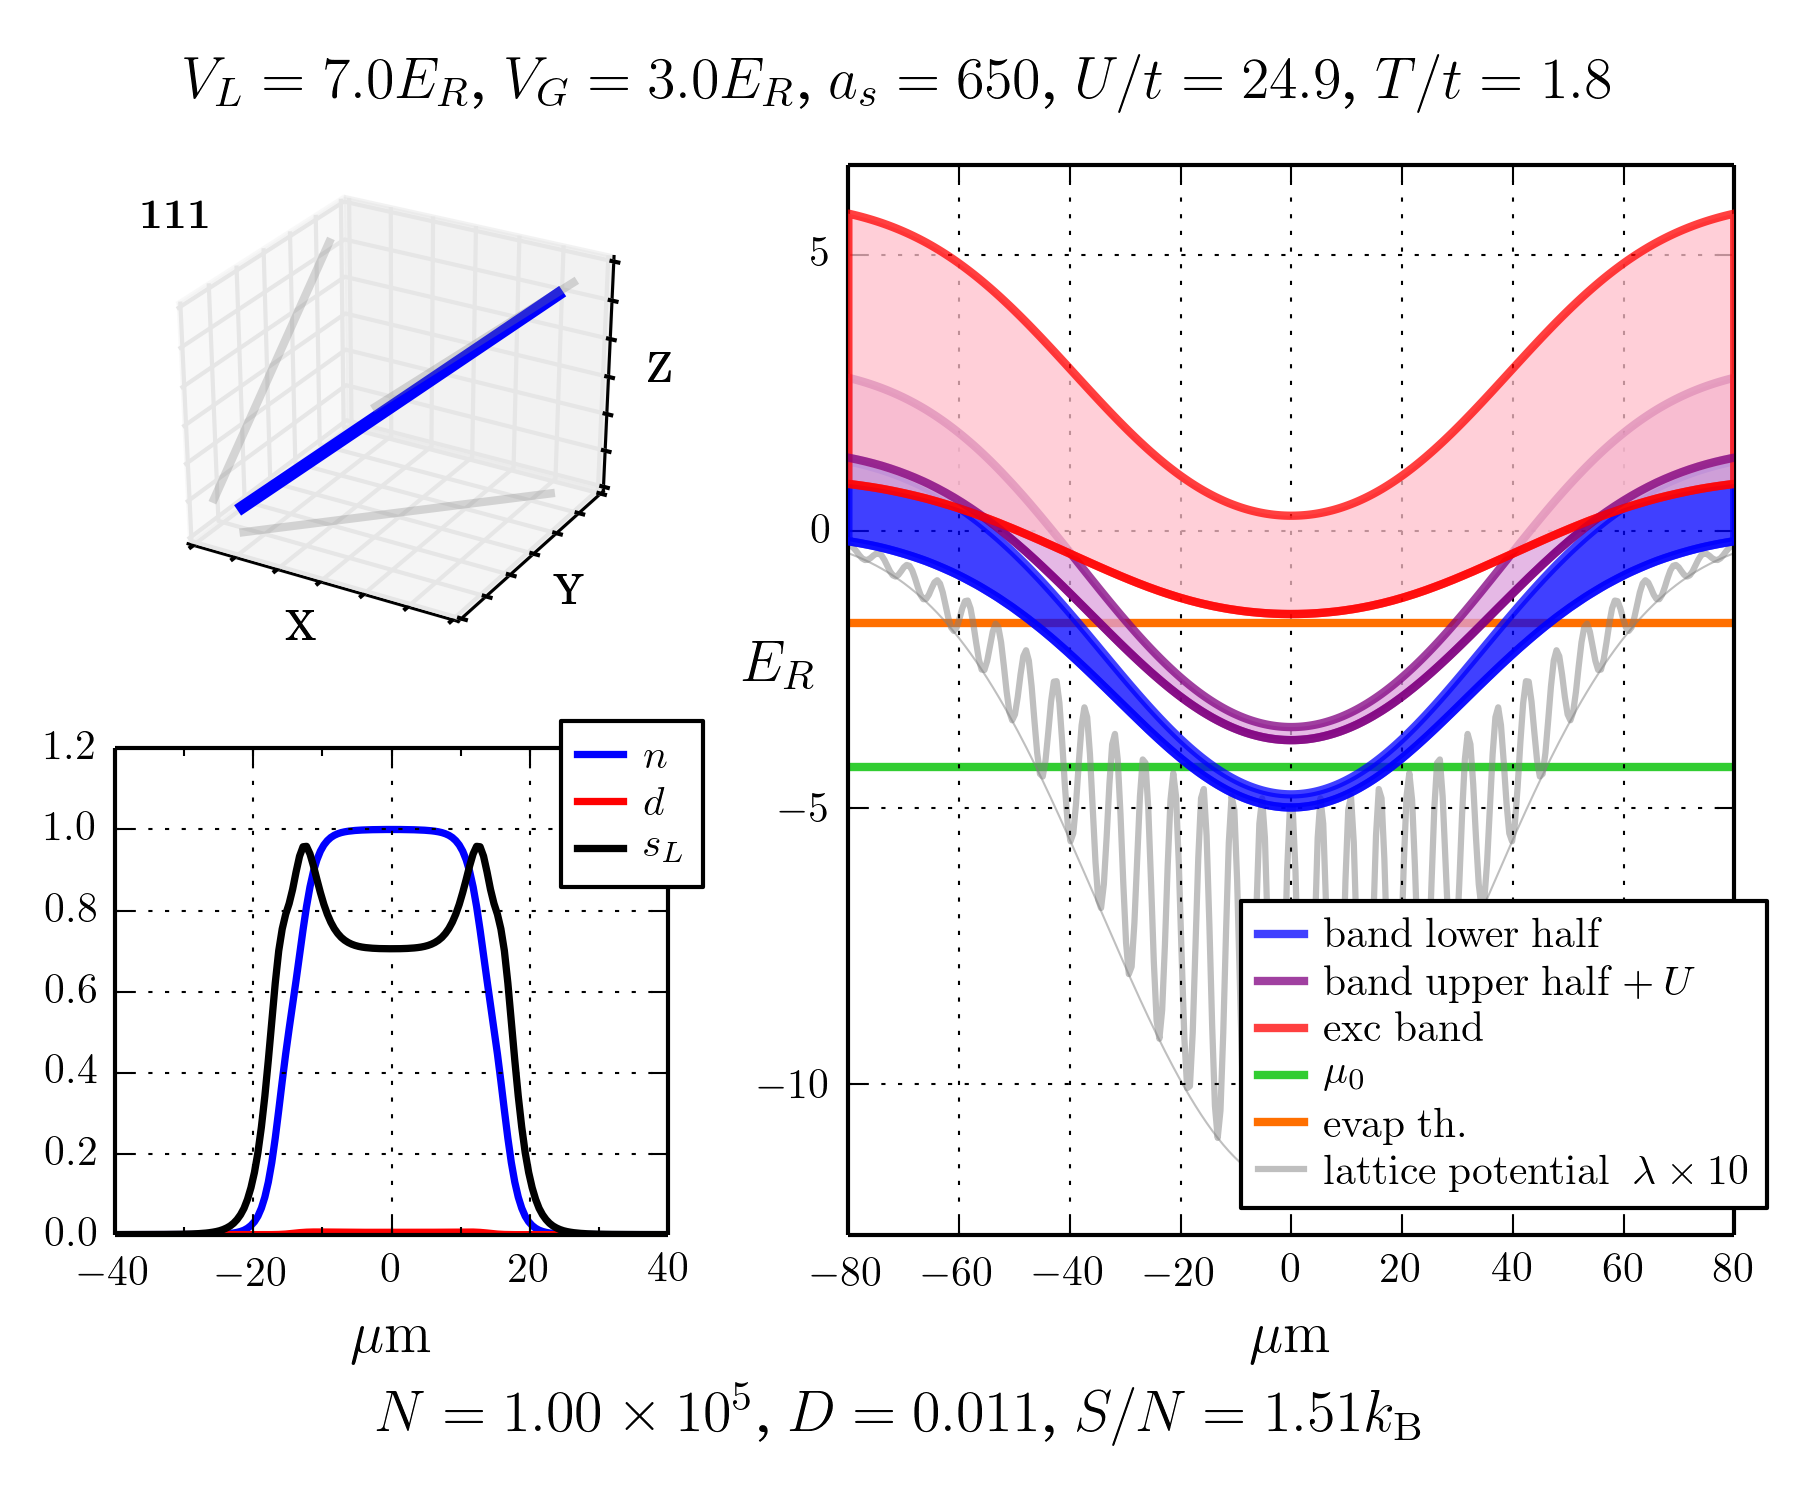
\includegraphics[width=\textwidth]{figures/ir47-gr40_7Er-comp3p05.png}
\caption{$w_{L}=47\,\mu$m and $w_{C}=40\,\mu$m with 3.05\,$E_{R}$ compensation.  }
                \label{fig:HTSE_enlarge-mott_b}
        \end{subfigure}
        ~        
        \begin{subfigure}[t]{0.32\textwidth}
                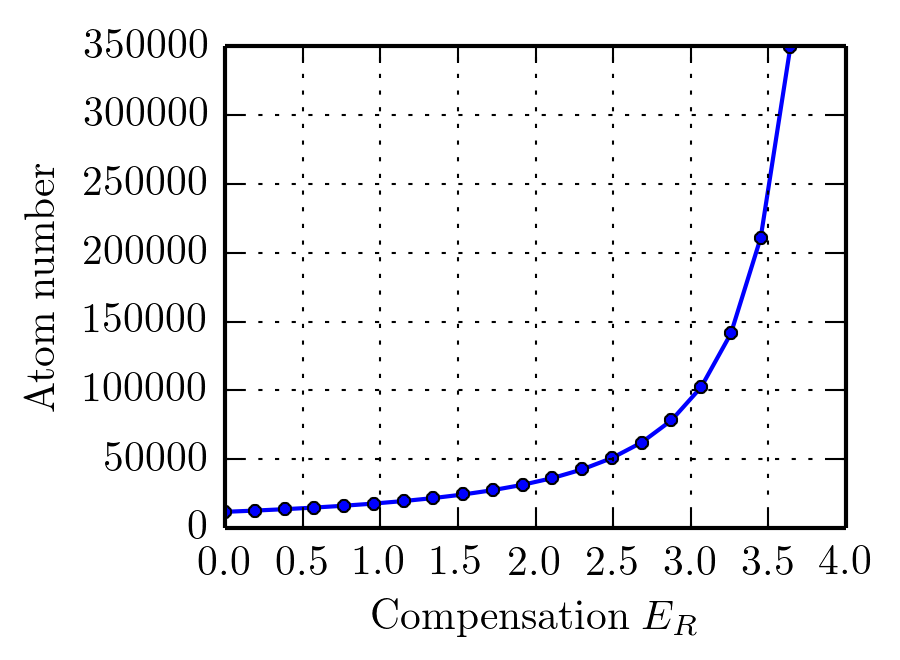
\includegraphics[width=\textwidth]{figures/enlarging_mott_state.png}
\caption{Atom number as a function of compensation illustrates the concept of enlarging the Mott state. }
                \label{fig:HSTE_enlarge-mott_c}
        \end{subfigure}
	\caption{  Illustrating the idea of enlarging the Mott state. 
}
\label{fig:HTSE_enlarge-mott}
\end{figure}


From what was discussed in \S\ref{sec:compare-big-small-waist}  we see that it
is also possible to reach an large Mott plateau for $N=350,000$ and without
compensation beams:  you just need to have larger lattice beam waists.  As we
saw there, the advantage of realizing the large Mott plateau with small lattice
beam waists and compensating beams is  that this system has a larger entropy
capacity  than the large-beam-waist-uncompensated counterpart.   

In addition to this entropy capacity advantage, the
small-beam-waist-compensated setup offers the possibility of evaporative
cooling since the chemical potential comes much closer to the energy threshold
for an atom escaping along one of the lattice beams.  We will address this
point in the following section.  


\section{ Evaporative cooling in a lattice }

If we refer back to Fig.~\ref{fig:HTSE_full-band-profiles}  we can see that on
the energy landscape plot we used an orange line to indicate the evaporation
threshold, that is the energy necessary for an atom to escape along one of the
lattice beams.  Comparing the two cases one sees that the small beam waist
compensated case has a global chemical potential (green line) that is much
closer to the evaporation threshold.

When evaporative cooling a thermal gas of atoms, one considers the parameter
$\eta=U_{\text{trap}}/\kb T$, where $U_{\text{trap}}$ is the energy threshold
for a particle leaving the trap (i.e. the trap depth) and $T$ is the
temperature of the gas.   The evaporation rate is suppressed by a factor
$\exp(-\eta)$ where  typically $\eta\sim10$ and, as the gas cools down, the trap
depth is reduced to force further evaporation~\cite{OHara2001}.  

For a deeply degenerate Fermi gas,  $T \ll T_{F}$, the evaporation rate is
given by~\cite{OHara2001}.
\begin{equation}
  \Gamma_{\text{evap}} \propto \gamma_{\text{coll}} \frac{T}{T_{F}} 
  \exp\left[ -   
  \frac{ U_{\text{trap}} - \kb T_{F} }{ \kb T }  \right ] 
\end{equation}
where $\gamma_{\text{coll}}$ is the classical collision rate evaluated at the
Fermi surface.  This can also be written as 
\begin{equation}
  \Gamma_{\text{evap}} \propto \gamma_{\text{coll}} \frac{T}{T_{F}}
  \exp\left[ \frac{1}{T/T_{F}} \right]  
  \exp\left[ -  \frac{1}{T/T_{F}} \left( \frac{U_{\text{trap}}}{\kb T_{F}} \right) \right] 
\end{equation}
We define $ \eta_{F} \equiv U_{\text{trap}}/\kb T_{F}$ and observe that 
\begin{equation}
  \Gamma_{\text{evap}} \propto \gamma_{\text{coll}} \frac{T}{T_{F}}
  \exp\left[ -  \frac{\eta_{F} - 1 }{ T/T_{F} } \right]
\label{eq:etaF}
\end{equation}
For the deeply degenerate gas, the $\eta$ factor which determines the
exponential suppression of the evaporation due to the trap depth is effectively
\begin{equation}
 \eta = \frac{\eta_{F} - 1 }{T/T_{F} } 
\end{equation}
Notice that the evaporation rate is additionally suppressed by a factor
$T/T_{F}$ due to Pauli blocking of one of the final states of a collision, which
occurs for $T\ll T_{F}$~\cite{OHara2001}.

We start by considering a red-detuned lattice with no extra confinement or
compensation.  We set  $n=1$ at the center of the sample and vary the waist of
the lattice beams.    From our knowledge of the potentials we can determine
$U_{\text{trap}}$, which in this case is the energy required for an atom to
escape along one of the lattice beams.   At a temperature of $T=1.8t$  we can
make the approximation $\kb T_{F} \approx \mu$, where $\mu$ is the global
chemical potential.  Figure~\ref{fig:etaF-no-comp_vary-wIR} shows $\eta_{F}$ as
a function of lattice beam waist, and also shows the number of atoms
required to achieve half-filling.   
\begin{figure}
    \centering
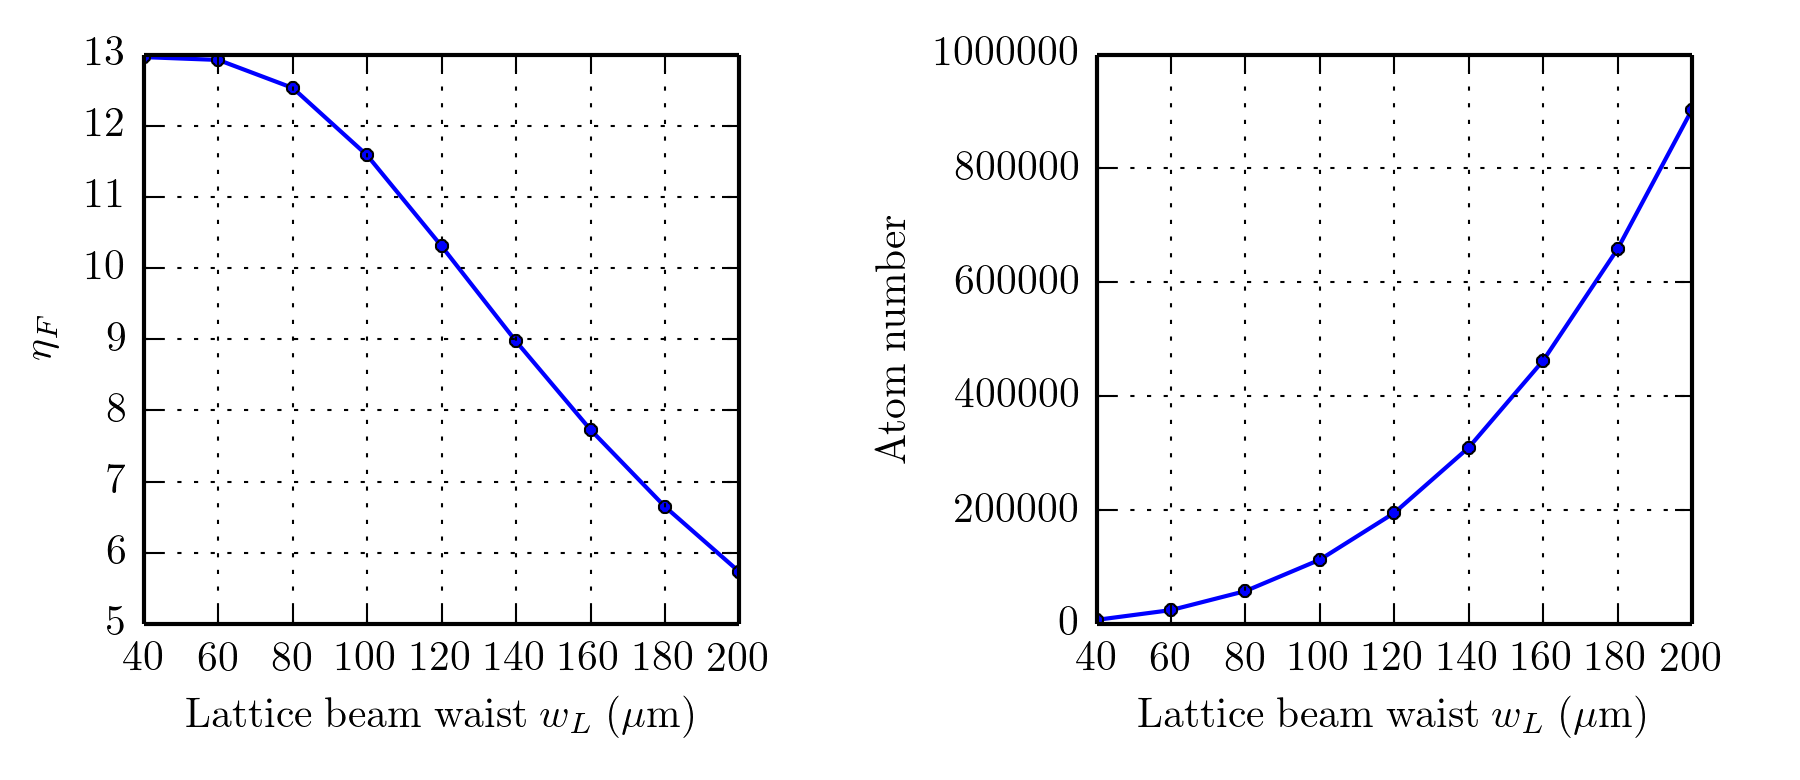
\includegraphics[width=0.8\textwidth]{figures/etaF-no-comp_vary-wIR.png}
\caption{$\eta_{F}$, an indicator of the exponential suppression of evaporation
is shown as a function of lattice beam waist for a red-detuned lattice without
any extra confinement or compensation. To determine $\eta_{F}$ the number of
atoms is adjusted such that filling is $n=1$ at the center.   The required
number is shown on the right.}\label{fig:etaF-no-comp_vary-wIR}
\end{figure}

In our experiment we can produce cold samples with $\sim$350,000 atoms.   As
can be seen in Fig.~\ref{fig:etaF-no-comp_vary-wIR} (and also was already shown
in Fig.~\ref{fig:HTSE_full-band-profiles_a}),  using a beam waist of
146\,$\mu$m would produce the confinement necessary to reach half-filling at
the center with $N=350,000$.  The flip side of this is that, for that beam
waist $\eta_{F}$ would be $\approx 8.5 $,  which for $T/T_{F}=0.1$ means that
the rate of evaporation would be suppressed by  
\begin{equation}
   \frac{T}{T_{F}}\exp\left[ - \frac{\eta_{F} - 1 }{T/T_{F} } 
 \right] \equiv \xi_{\text{evap}}\approx 10^{-34} 
\end{equation} 

Going back to our current setup, which has $w_{L}=47\,\mu$m and
$w_{C}=40\,\mu$m,  with 350,000 atoms; we can achieve half filling if we use
3.64$E_{R}$ of compensation.  This yields $\eta_{F} \approx 2.95$.  This is a
lot better than the large-beam-waist-uncompensated case, however the suppression
factor for the rate of evaporative cooling is still very small.  For our
current setup it would be
\begin{equation}
 \xi_{\text{evap}} = 3.4\times 10^{-10} 
\end{equation}

Under typical evaporation conditions $\eta=10$, and for a non-degenerate sample
we have 
\begin{equation}
 \xi_{\text{evap}} = e^{-10} = 4.5\times 10^{-5} 
\end{equation}
We conclude that our current setup would  have an evaporation rate \textbf{five
orders of magnitude smaller} compared to the typical evaporative cooling rate
for a thermal gas (given the same rate of elastic collisions
$\gamma_{\text{coll}}$).   In addition, in order to get a more realistic
estimate we would need to incorporate the implications of the chemical
potential being in a gapped region of the spectrum (for half-filling the chemical
potential is at the center of the Mott gap) which should further reduce the
evaporation rate.  

We now explore the entire parameter space, where we allow the lattice and
compensation beam waists to vary.   We set the chemical potential so that $n=1$
at the center of the sample,  we do this because half-filling is a prerequisite
to achieve Mott or N\'{e}el states.   We attempt to find a compensation such
that $N=350,000$ atoms.  For some values of the beam waists that is not
possible because it would lead to either spilling atoms from the
trap\footnote{In cases when $w_{C}>w_{L}$.} or to the creation of a negative
curvature in the confinement at the center of our sample\footnote{In cases when
$w_{C} < w_{L}$.  We also refer to this as making a donut}.  
\begin{figure}
    \centering 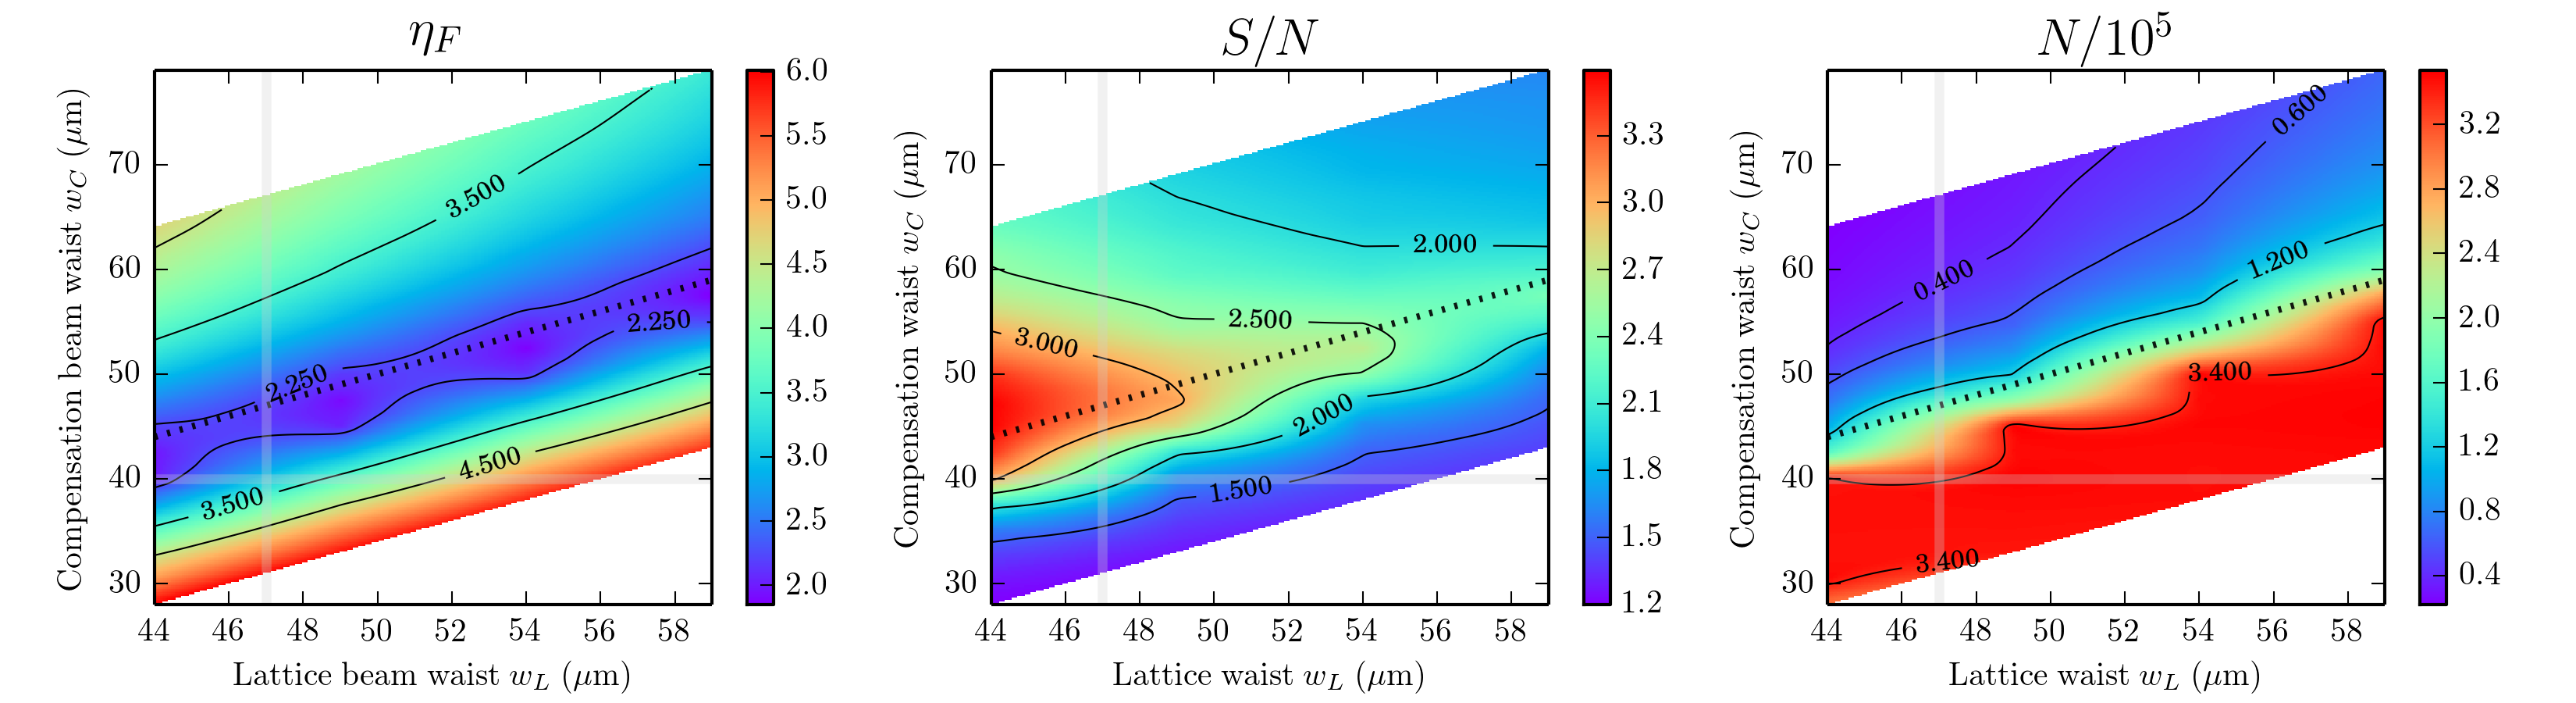
\includegraphics[width=\textwidth]{figures/etaF-wIRwGR.png}
\caption{$\eta_{F}$ and $S/N$ and $N$ are plotted for various lattice and
compensation beam waists.  The filling is set to $n=1$ at the center. The
compensation depth is adjusted so that  $N=350,000$ if it is possible, otherwise
it is set to maximize the atom number without spilling any atoms form the trap
or creating a Mexican hat at the center of the potential.  The dotted line in
the plots corresponds to $w_{L}=w_{C}$.  The current values of our
experimental setup are shown as gray lines,  such that the intersection between
these two gray lines represents our current conditions. }
\label{fig:etaF-wIRwGR}
\end{figure}

The results of the
exploration of the beam waist parameter space are shown in
Fig.~\ref{fig:etaF-wIRwGR}.  The main points that stand out are
\begin{itemize}
\item  An optimal value of $\eta_{F}$ is achieved for $w_{L}\approx w_{C}$.  
\item  At $w_{L} \approx w_{C}$, smaller beam waists give better entropy capacity 
\item The atom number can only reach 350,000 if $w_{C} < w_{L}$, such as in our
current setup.  Otherwise the atom number is limited, being smaller for larger
$w_{C}$.
\end{itemize}


To get another look at the results, on Fig.~\ref{fig:etaF-wIRwGR-lines} we plot
$\eta_{F}$, $S/N$, and $N$  as a function of $w_{C}$ for three different values
of $w_{L}$.  The evaporation factor is optimized for nearly equal beam waists
and the entropy capacity also peaks up around there. 
\begin{figure}
    \centering
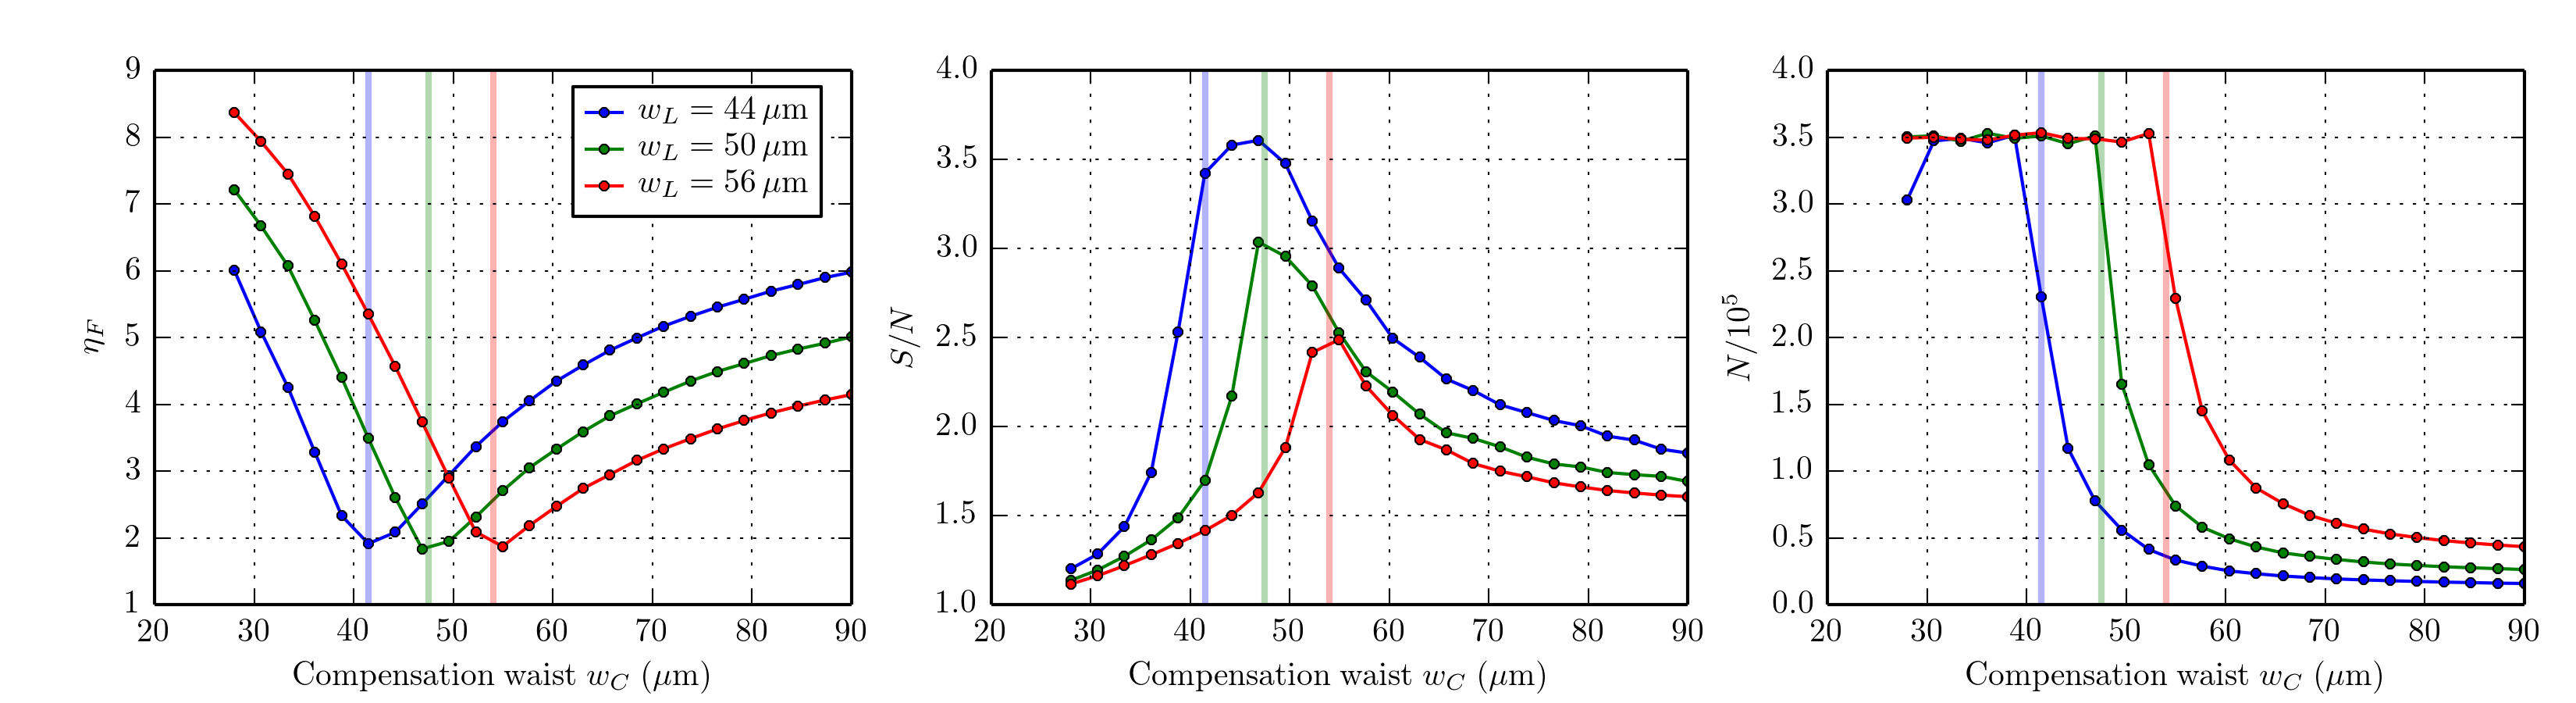
\includegraphics[width=\textwidth]{figures/etaF-wIRwGR-lines.png} \caption{
$\eta_{F}$, $S/N$, and $N$ as a function of $w_{C}$ for various values of $w_{L}$.  }
\label{fig:etaF-wIRwGR-lines}
\end{figure}
Given this observation,  we now set $w_{L}=w_{C}$ and vary both together  to see
if it is favorable to make smaller or larger beam waists.  This is shown in
Fig.~\ref{fig:etaF-wIR=wGR}.  The main observations are:
\begin{itemize}
\item  For beam waists up to $\approx68\,\mu$m one can keep getting lower
$\eta_{F}$ by making the beam waists larger.  This trend would continue if we
had an unlimited number of atoms, however beyond $\approx68\,\mu$m the number
of atoms required to fill the trap goes above our cap of 350,000 atoms.  
\item
For larger beam waists the entropy capacity is always lower, so the choice of
beam waist will be a compromise between $\eta_{F}$ and the entropy capacity. 
\end{itemize} 
\begin{figure}
    \centering 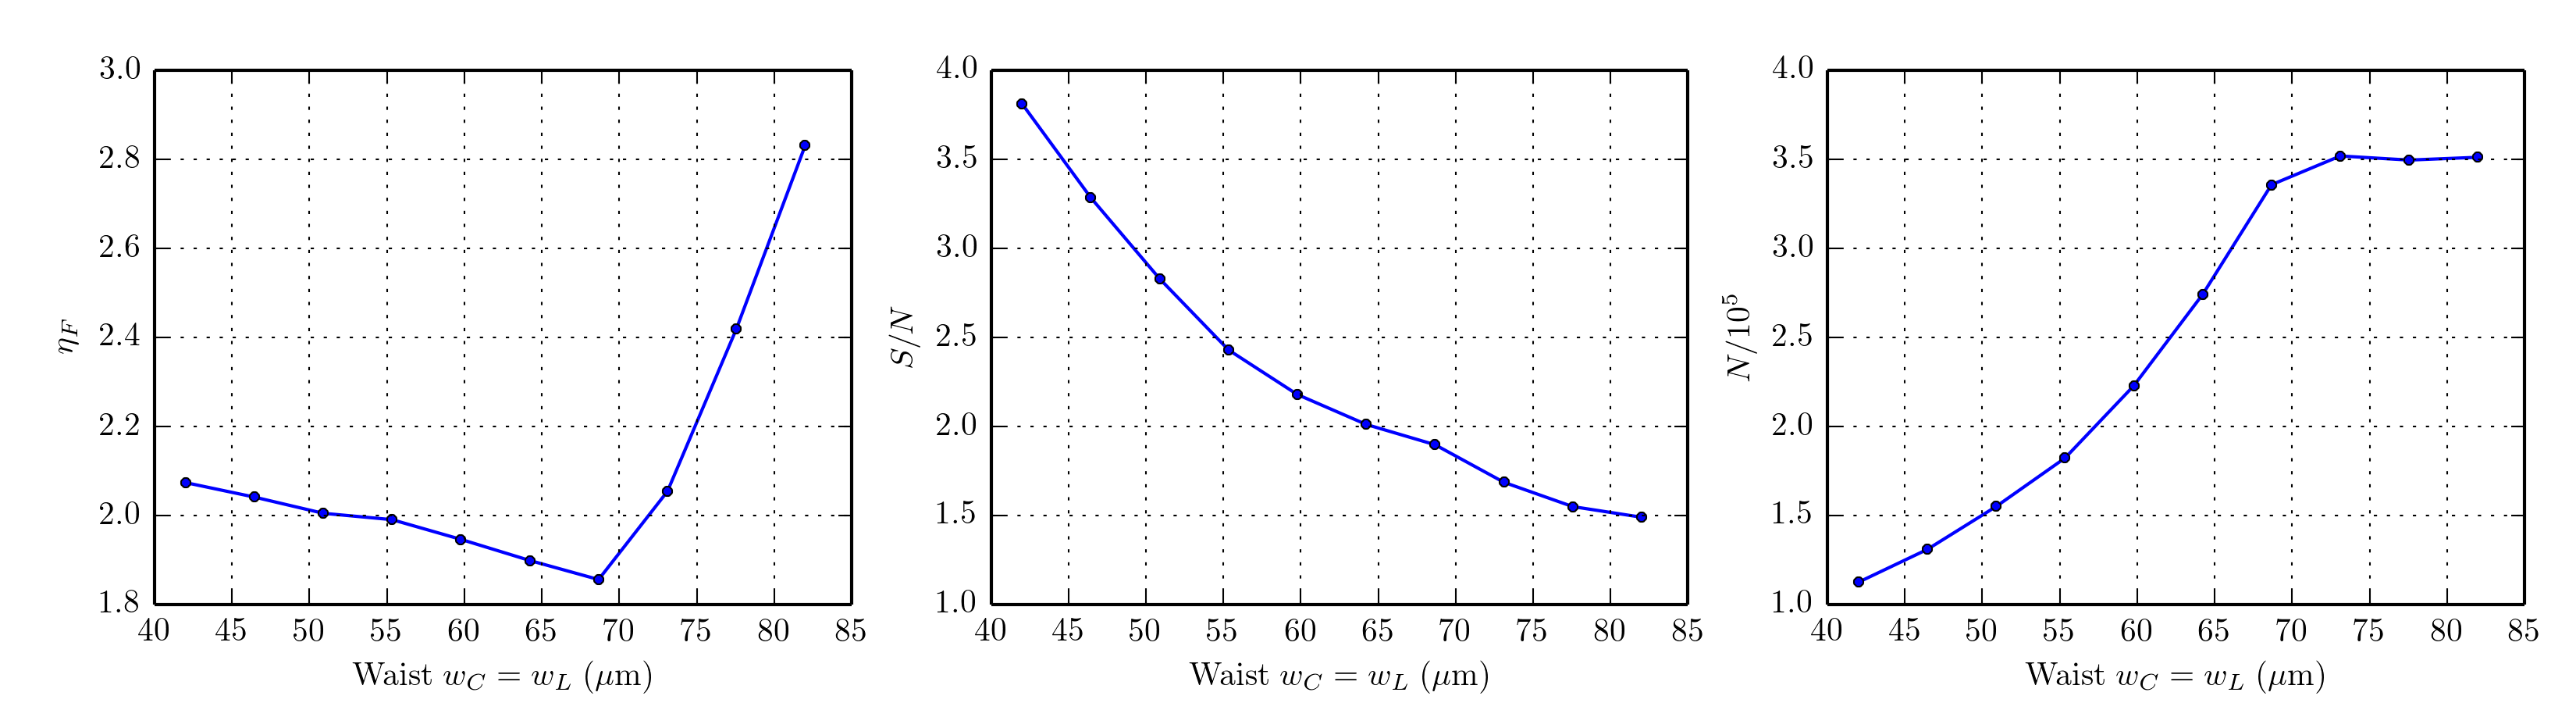
\includegraphics[width=\textwidth]{figures/etaF-wIR=wGR.png}
\caption{ $\eta_{F}$ and $S/N$ as a function of beam waist for $w_{L}=w_{C}$.
Results are shown for various atom numbers.  }
\label{fig:etaF-wIR=wGR}
\end{figure}

%In my opinion, the choice of beam waist should exploit the number of atoms that
%we have at our disposal


The results shown in Figs.~\ref{fig:etaF-wIR=wGR},~\ref{fig:etaF-wIRwGR-lines}
show that it is desirable to have equal lattice and compensation beam waists.
The choice of their value is a compromise between the achievable $\eta_{F}$ and
the entropy capacity, given by $S/N$.   Another important experimental
constraint is the available of power at the lattice and compensation
wavelengths, which is a bigger issue for larger beam waists.  In that case
larger power is necessary to achieve the required potential depths.   The
compensation power needed to compensate a 7\,$E_{R}$ lattice and the lattice
power needed to make a 40\,$E_{R}$ deep lattice\footnote{If we want to freeze
out tunneling in the lattice we required depths as large as 40\,$E_{R}$ where
the tunneling rate goes down to 3\,Hz.  We currently ``lock'' the lattice at
20\,$E_{R}$ for our Bragg scattering measurements.  At 20\,$E_{R}$ the
tunneling rate is 72\,Hz. This is good enough for Bragg scattering, but not
good enough for measurements that take longer, such as associating through the
narrow Feshbach resonance to measure double occupancies. } are shown in
Fig.~\ref{fig:green-power-wIR=wGR}.   With this in mind and our available
powers we can safely realize any choice of beam waists below $65\,\mu$m. 
\begin{figure}
    \centering
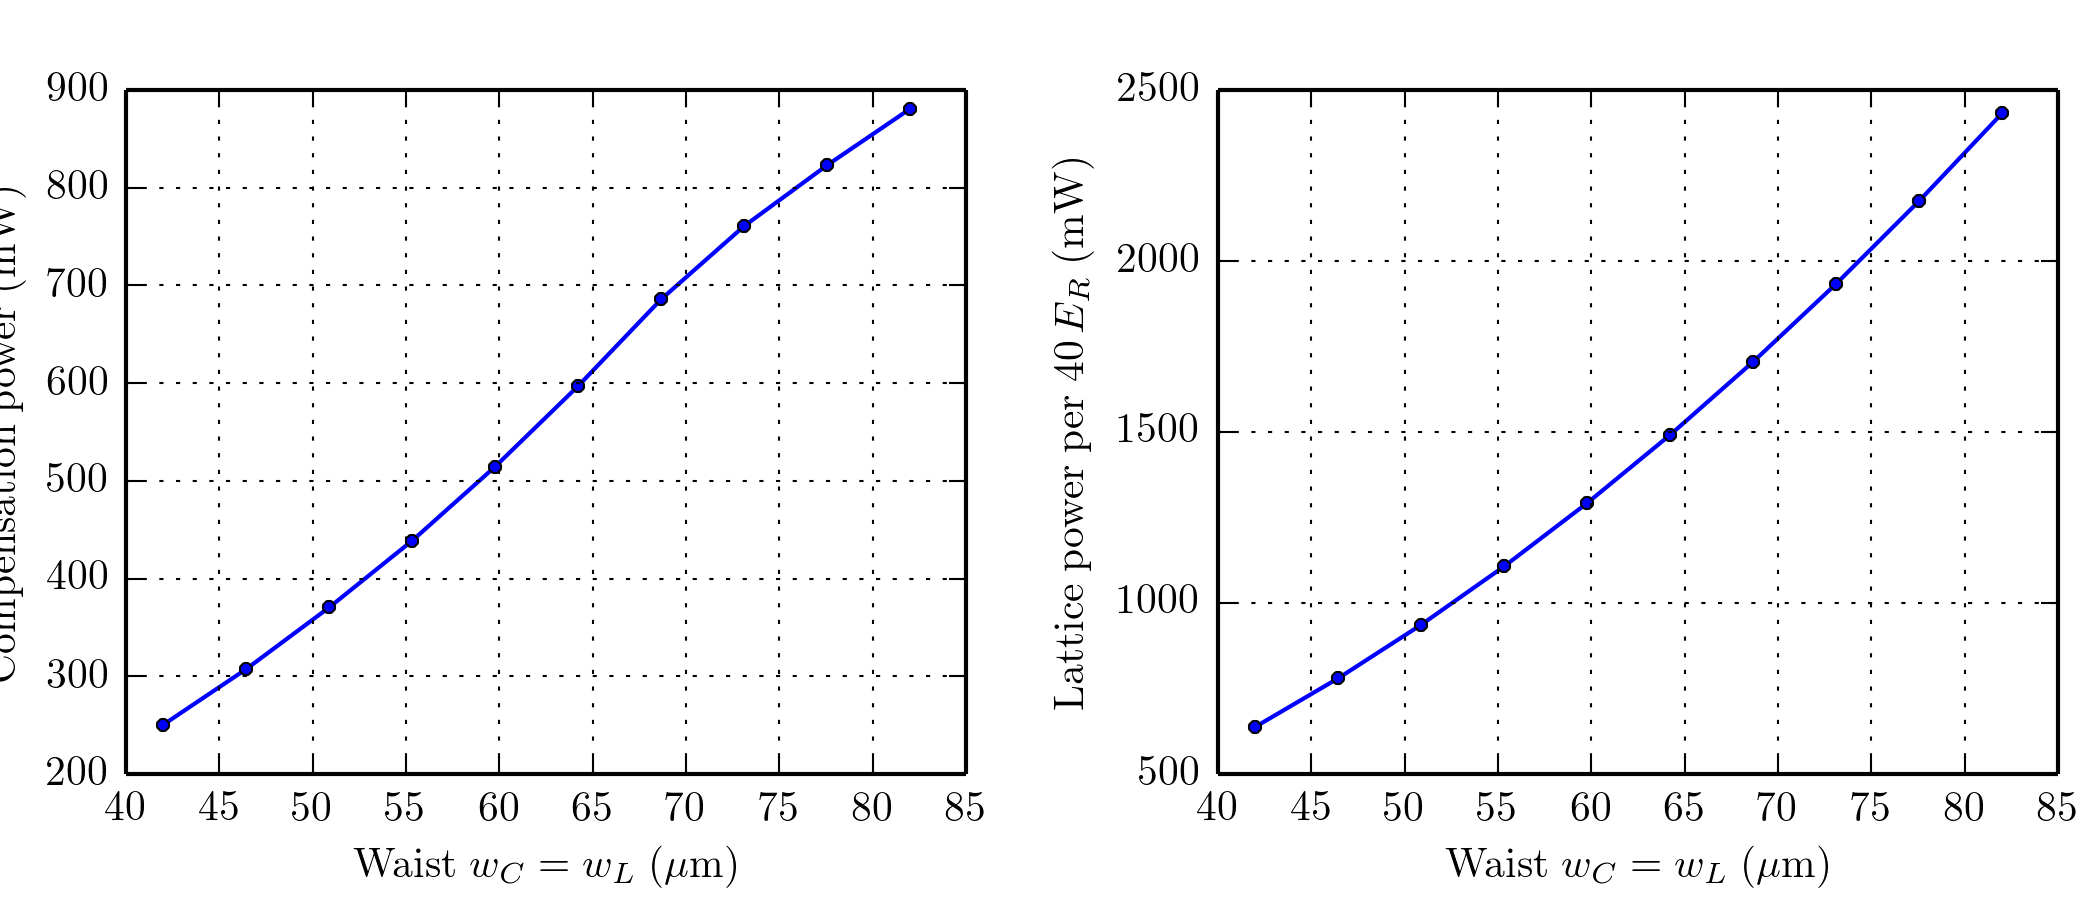
\includegraphics[width=0.7\textwidth]{figures/green-power-wIR=wGR.png}
\caption{ Compensation power required to compensate a 7\,$E_{R}$ lattice and
lattice powered required to achieve a 40\,$E_{R}$ lattice depth.  }
\label{fig:green-power-wIR=wGR}
\end{figure}

To fully exploit the atom number that we can produce in our experiment our
opinion is to go to the larger lattice beam waists,  so we recommend values of
$w_{L}=w_{C}=65\,\mu$m.   These proposed parameters  would change the
evaporation factor and entropy capacity and number capacity of our setup
according to the following table:
\begin{center}
\begin{tabular}{ c|c|c|c|c|c}
   &  $w_{L}\,(\mu\mathrm{m})$ & $w_{C}\,(\mu\mathrm{m})$ 
   & $\eta_{F}$  & $\xi_{\text{evap}}$ &  $S/N$  \\ \hline 
 Current setup &  47 & 40  &  2.95 & $3.4\times 10^{-10}$  &   1.94  \\ 
 Proposed change & 65 & 65  &  1.52 & $1.36\times 10^{-5}$  &   1.99  \\
\end{tabular}
\end{center}
We see that for the optimal beam waist ratio a value of
$\xi_{\text{evap}}\sim10^{-5}$ may be reached that could lead to reasonable
rates of evaporation in the lattice.  A comparison of our current setup and
this proposed scenario is shown in Fig.~\ref{fig:etaF-before-after}. 
\begin{figure}
        \centering
        \begin{subfigure}[t]{0.45\textwidth}
		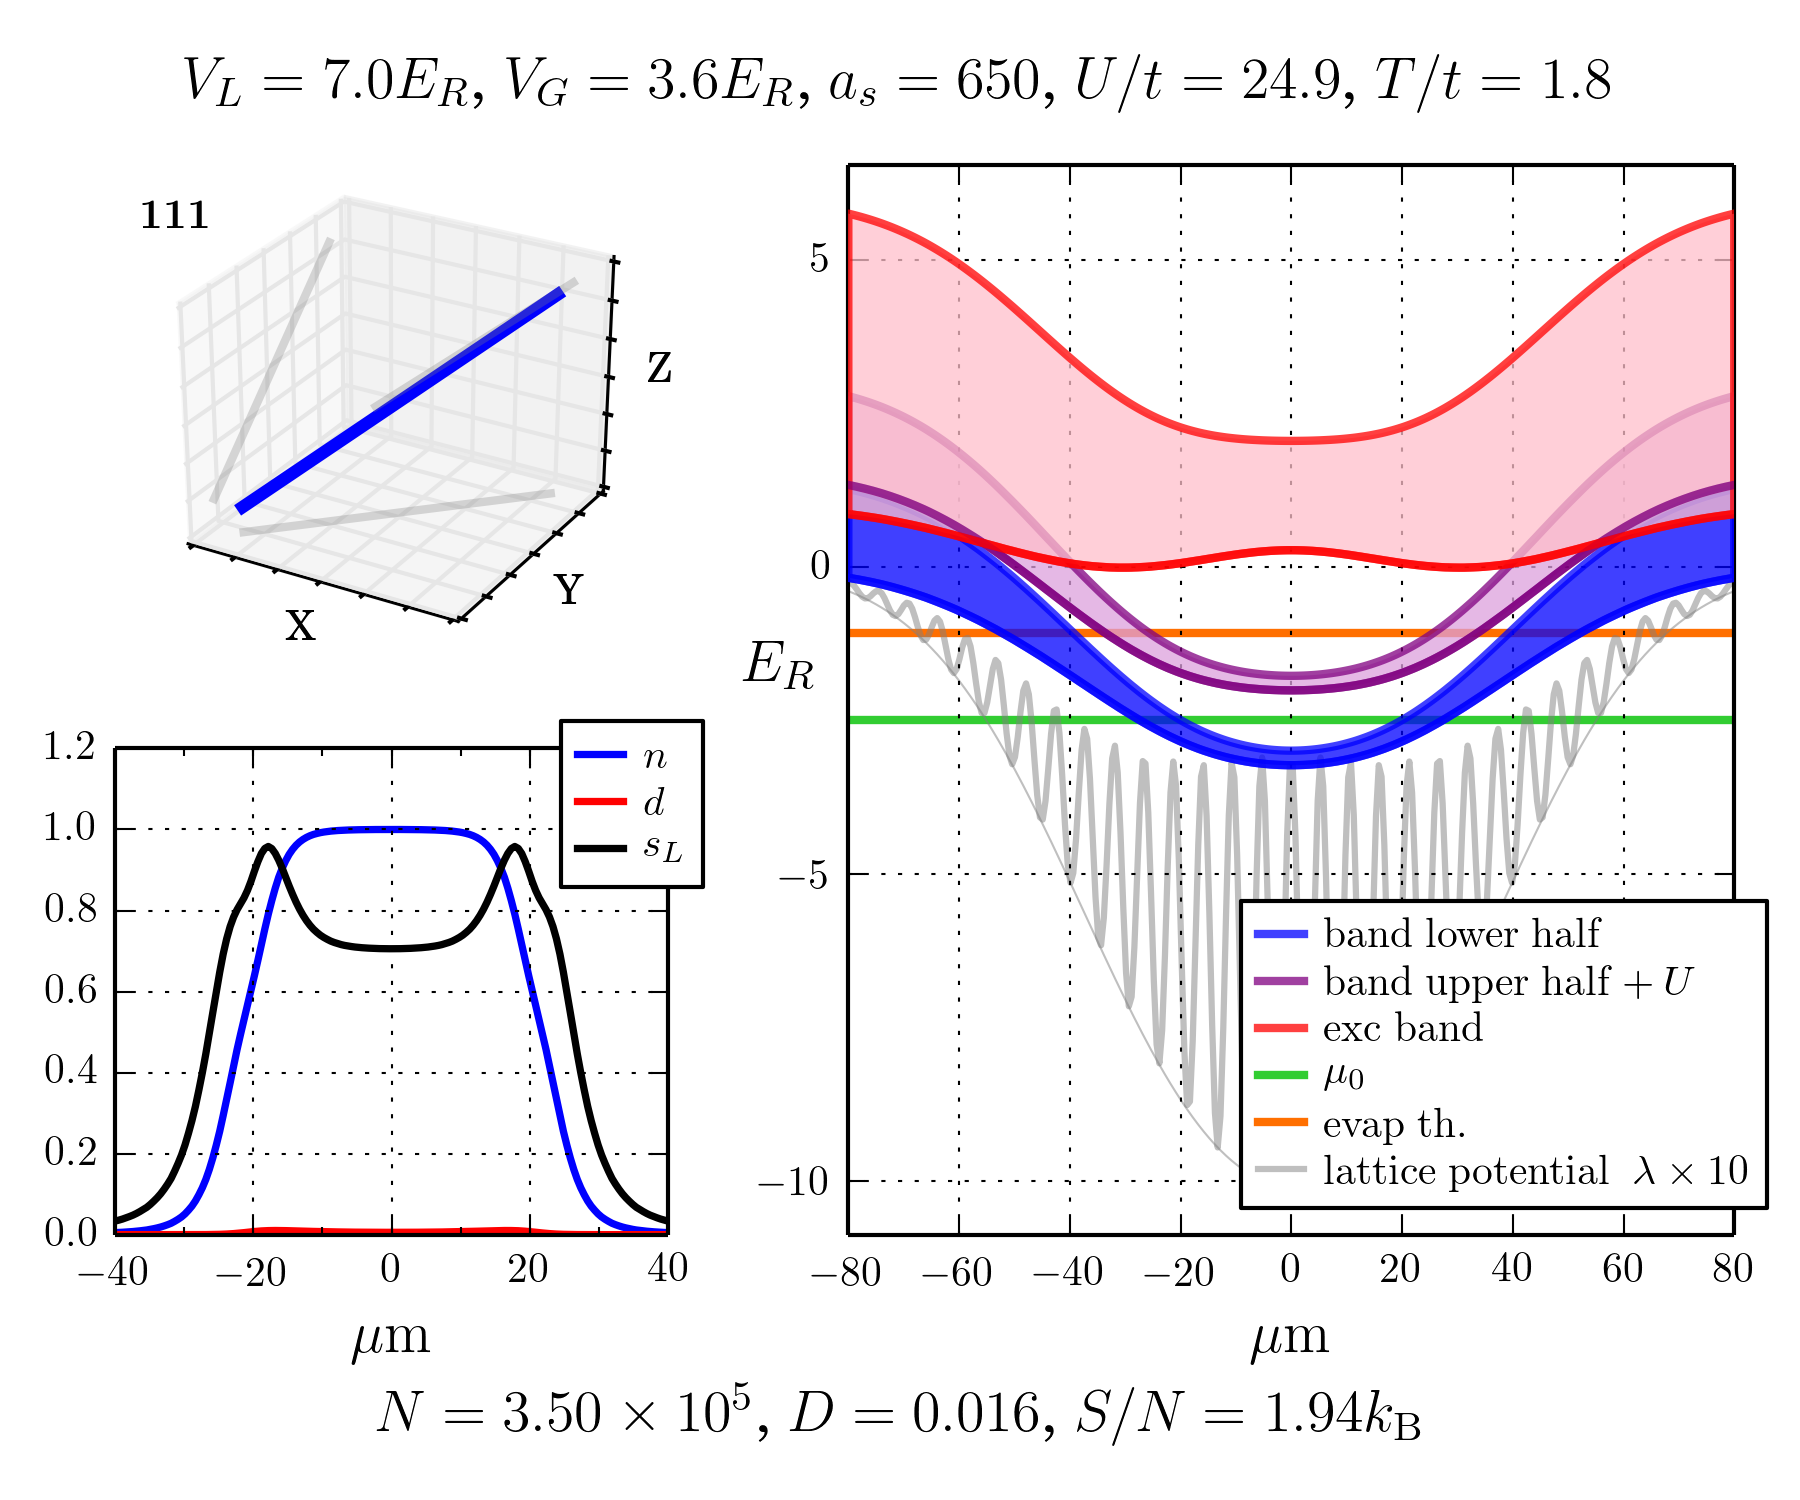
\includegraphics[width=\textwidth]{figures/ir47-gr40_7Er-comp3p642.png}
\caption{ $w_{L} = 47\,\mu$m and $w_{C}=40\,\mu$m.  Compensation is chosen so
that unit filling is achieved at the center for an atom number of 350,000. }
        \end{subfigure}
        ~ %add desired spacing between images, e. g. ~, \quad, \qquad etc.
          %(or a blank line to force the subfigure onto a new line)
        \begin{subfigure}[t]{0.45\textwidth}
		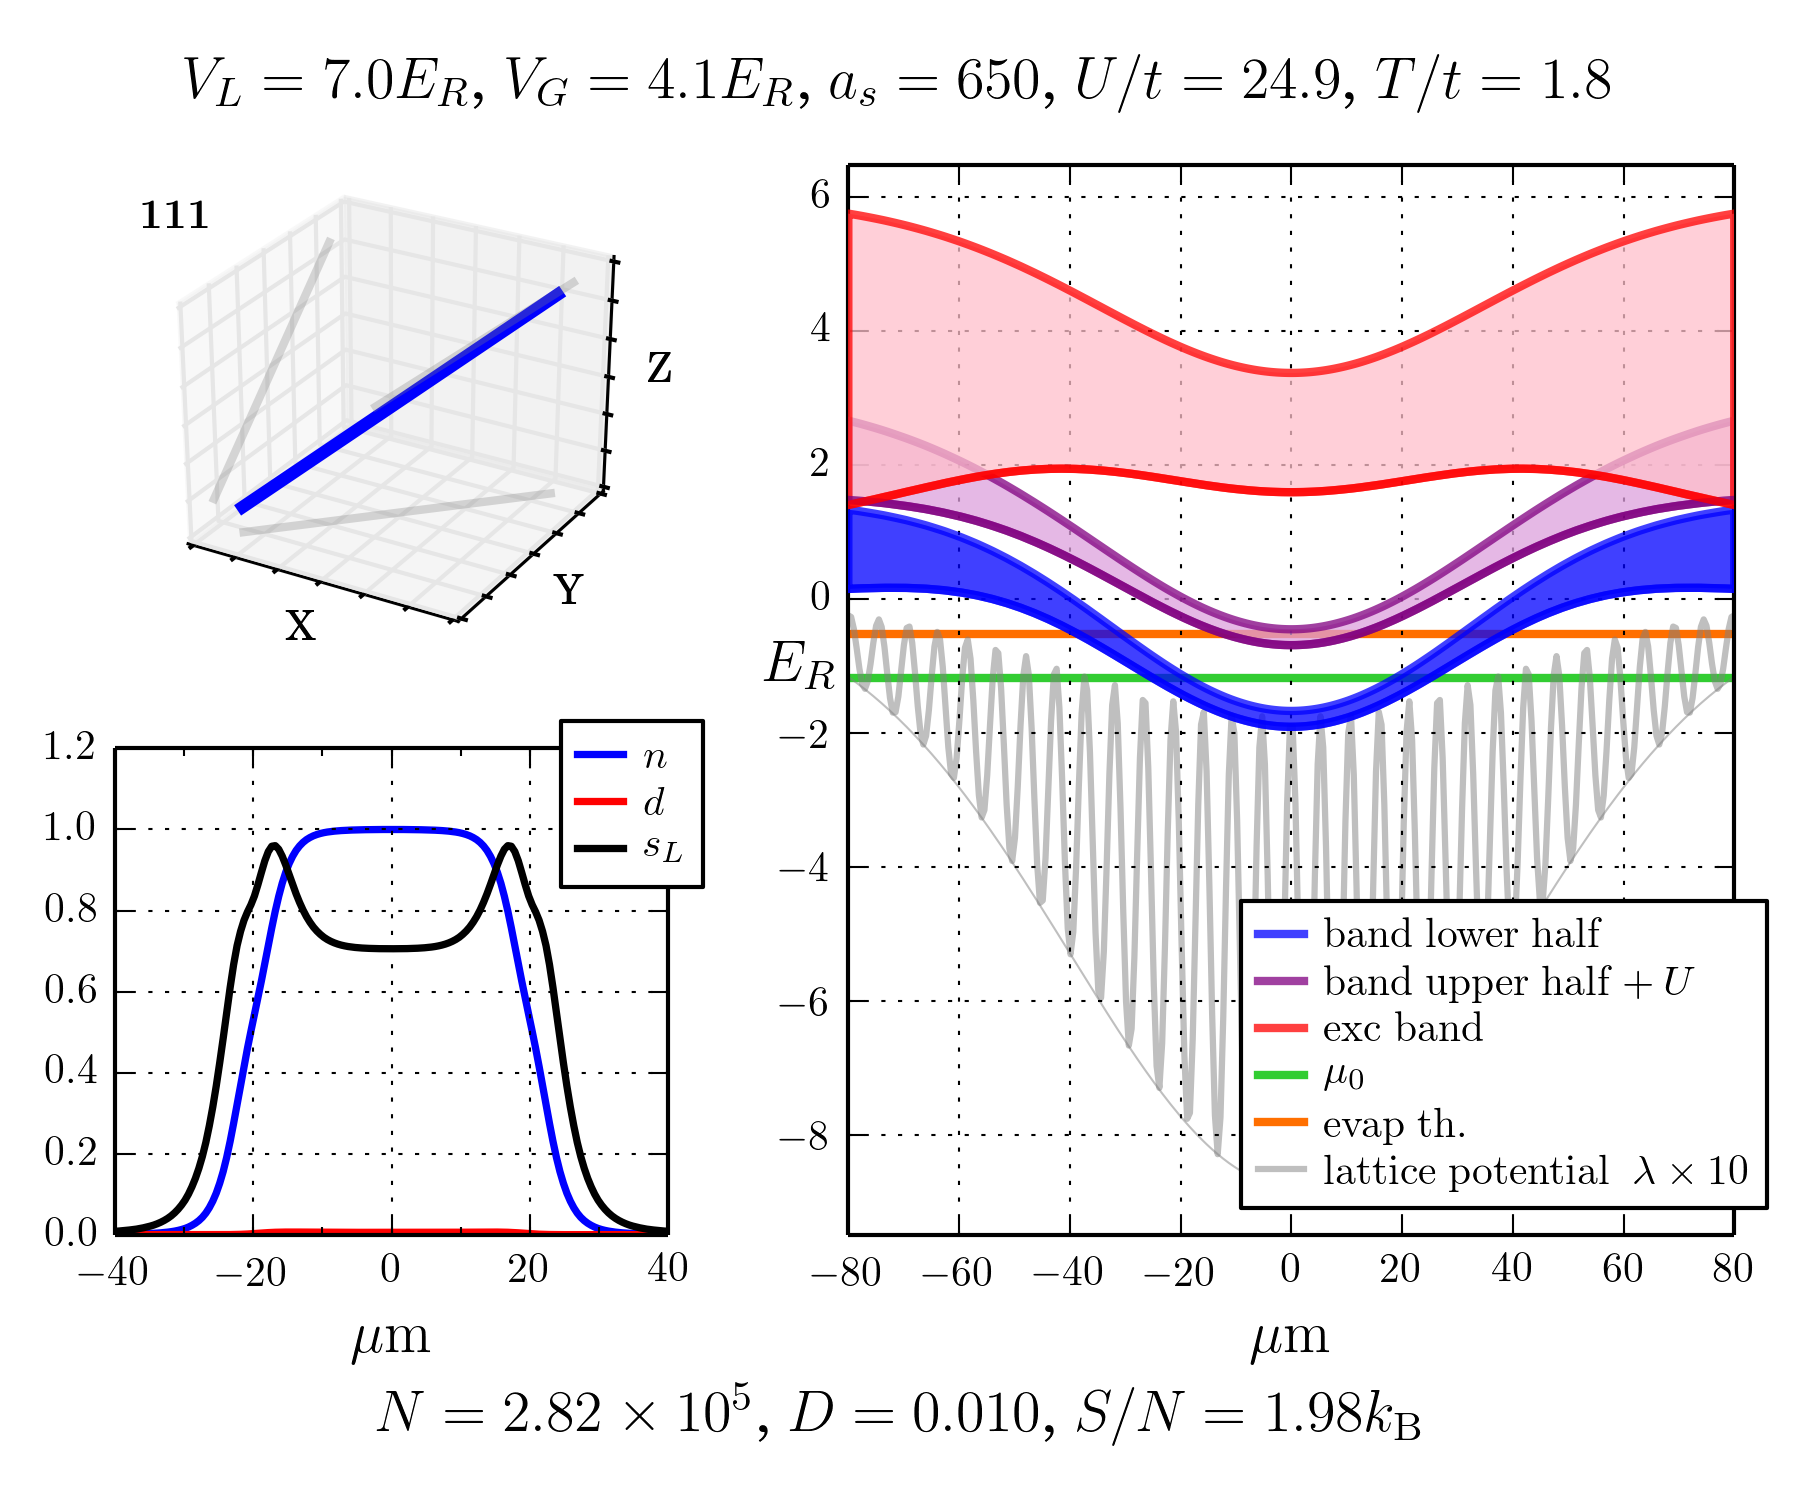
\includegraphics[width=\textwidth]{figures/ir65-gr65_7Er-comp4p08.png}
\caption{ $w_{L} = 65\,\mu$m and $w_{C}=65\,\mu$m.  Atom number maxes out at 284,000 atoms. }
        \end{subfigure}%
	\caption{Full trap profiles of band structure and thermodynamic
quantities for our current setup and the proposed setup with equal beam waists.} 
\label{fig:etaF-before-after}
\end{figure}

 



 
\section{ Conclusions }

\newpage

\bibliographystyle{osa}
\bibliography{latt_evap}

\end{document}




